\documentclass[twoside]{book}

% Packages required by doxygen
\usepackage{calc}
\usepackage{doxygen}
\usepackage{graphicx}
\usepackage[utf8]{inputenc}
\usepackage{makeidx}
\usepackage{multicol}
\usepackage{multirow}
\usepackage{textcomp}
\usepackage[table]{xcolor}

% Font selection
\usepackage[T1]{fontenc}
\usepackage{mathptmx}
\usepackage[scaled=.90]{helvet}
\usepackage{courier}
\usepackage{amssymb}
\usepackage{sectsty}
\renewcommand{\familydefault}{\sfdefault}
\allsectionsfont{%
  \fontseries{bc}\selectfont%
  \color{darkgray}%
}
\renewcommand{\DoxyLabelFont}{%
  \fontseries{bc}\selectfont%
  \color{darkgray}%
}

% Page & text layout
\usepackage{geometry}
\geometry{%
  a4paper,%
  top=2.5cm,%
  bottom=2.5cm,%
  left=2.5cm,%
  right=2.5cm%
}
\tolerance=750
\hfuzz=15pt
\hbadness=750
\setlength{\emergencystretch}{15pt}
\setlength{\parindent}{0cm}
\setlength{\parskip}{0.2cm}
\makeatletter
\renewcommand{\paragraph}{%
  \@startsection{paragraph}{4}{0ex}{-1.0ex}{1.0ex}{%
    \normalfont\normalsize\bfseries\SS@parafont%
  }%
}
\renewcommand{\subparagraph}{%
  \@startsection{subparagraph}{5}{0ex}{-1.0ex}{1.0ex}{%
    \normalfont\normalsize\bfseries\SS@subparafont%
  }%
}
\makeatother

% Headers & footers
\usepackage{fancyhdr}
\pagestyle{fancyplain}
\fancyhead[LE]{\fancyplain{}{\bfseries\thepage}}
\fancyhead[CE]{\fancyplain{}{}}
\fancyhead[RE]{\fancyplain{}{\bfseries\leftmark}}
\fancyhead[LO]{\fancyplain{}{\bfseries\rightmark}}
\fancyhead[CO]{\fancyplain{}{}}
\fancyhead[RO]{\fancyplain{}{\bfseries\thepage}}
\fancyfoot[LE]{\fancyplain{}{}}
\fancyfoot[CE]{\fancyplain{}{}}
\fancyfoot[RE]{\fancyplain{}{\bfseries\scriptsize Generated on Sat May 7 2016 17\-:02\-:58 for Multimeter G\-U\-I by Doxygen }}
\fancyfoot[LO]{\fancyplain{}{\bfseries\scriptsize Generated on Sat May 7 2016 17\-:02\-:58 for Multimeter G\-U\-I by Doxygen }}
\fancyfoot[CO]{\fancyplain{}{}}
\fancyfoot[RO]{\fancyplain{}{}}
\renewcommand{\footrulewidth}{0.4pt}
\renewcommand{\chaptermark}[1]{%
  \markboth{#1}{}%
}
\renewcommand{\sectionmark}[1]{%
  \markright{\thesection\ #1}%
}

% Indices & bibliography
\usepackage{natbib}
\usepackage[titles]{tocloft}
\setcounter{tocdepth}{3}
\setcounter{secnumdepth}{5}
\makeindex

% Hyperlinks (required, but should be loaded last)
\usepackage{ifpdf}
\ifpdf
  \usepackage[pdftex,pagebackref=true]{hyperref}
\else
  \usepackage[ps2pdf,pagebackref=true]{hyperref}
\fi
\hypersetup{%
  colorlinks=true,%
  linkcolor=blue,%
  citecolor=blue,%
  unicode%
}

% Custom commands
\newcommand{\clearemptydoublepage}{%
  \newpage{\pagestyle{empty}\cleardoublepage}%
}


%===== C O N T E N T S =====

\begin{document}

% Titlepage & ToC
\hypersetup{pageanchor=false}
\pagenumbering{roman}
\begin{titlepage}
\vspace*{7cm}
\begin{center}%
{\Large Multimeter G\-U\-I }\\
\vspace*{1cm}
{\large Generated by Doxygen 1.8.6}\\
\vspace*{0.5cm}
{\small Sat May 7 2016 17:02:58}\\
\end{center}
\end{titlepage}
\clearemptydoublepage
\tableofcontents
\clearemptydoublepage
\pagenumbering{arabic}
\hypersetup{pageanchor=true}

%--- Begin generated contents ---
\chapter{Main Page}
\label{index}\hypertarget{index}{}Multimeter G\-U\-I G\-U\-I for the R\-S-\/232 mode of the Radio Shack 22-\/812. Copyright (C) 2016 F\-J Salguero

This program is free software\-: you can redistribute it and/or modify it under the terms of the G\-N\-U General Public License as published by the Free Software Foundation, either version 3 of the License, or (at your option) any later version.

This program is distributed in the hope that it will be useful, but W\-I\-T\-H\-O\-U\-T A\-N\-Y W\-A\-R\-R\-A\-N\-T\-Y; without even the implied warranty of M\-E\-R\-C\-H\-A\-N\-T\-A\-B\-I\-L\-I\-T\-Y or F\-I\-T\-N\-E\-S\-S F\-O\-R A P\-A\-R\-T\-I\-C\-U\-L\-A\-R P\-U\-R\-P\-O\-S\-E. See the G\-N\-U General Public License for more details.

You should have received a copy of the G\-N\-U General Public License along with this program. If not, see \href{http://www.gnu.org/licenses/}{\tt http\-://www.\-gnu.\-org/licenses/}. 
\chapter{multimeter\-G\-U\-I}
\label{md__r_e_a_d_m_e}
\hypertarget{md__r_e_a_d_m_e}{}
G\-U\-I for the Radio Shack 22-\/812 multimeter when used in R\-S232 mode.

This is a Q\-T G\-U\-I to interface the R\-S 22-\/812. It has been developed with Q\-T5 in Open\-Suse Leap.

This code is \char`\"{}as-\/is\char`\"{}. No waranty or responsability is assumed by the author. You can use your code for any non-\/commercial purposes, and modify it as you wish with the only condition of licensing it with the same conditions. If you find it useful, make any change or have any suggestion, I will appreciate your input. 
\chapter{Todo List}
\label{todo}
\hypertarget{todo}{}

\begin{DoxyRefList}
\item[\label{todo__todo000001}%
\hypertarget{todo__todo000001}{}%
Member \hyperlink{main_8cpp_a0ddf1224851353fc92bfbff6f499fa97}{main} (int argc, char $\ast$argv\mbox{[}\mbox{]})]Add display controls.  
\item[\label{todo__todo000002}%
\hypertarget{todo__todo000002}{}%
Member \hyperlink{class_main_window_a8b244be8b7b7db1b08de2a2acb9409db}{Main\-Window\-:\-:Main\-Window} (Q\-Widget $\ast$parent=0)]\-: Temporary. It has to be set automatically. 
\end{DoxyRefList}
\chapter{Namespace Index}
\section{Namespace List}
Here is a list of all namespaces with brief descriptions\-:\begin{DoxyCompactList}
\item\contentsline{section}{\hyperlink{namespace_ui}{Ui} }{\pageref{namespace_ui}}{}
\end{DoxyCompactList}

\chapter{Hierarchical Index}
\section{Class Hierarchy}
This inheritance list is sorted roughly, but not completely, alphabetically\-:\begin{DoxyCompactList}
\item \contentsline{section}{Flags}{\pageref{struct_flags}}{}
\item Q\-Graphics\-Item\begin{DoxyCompactList}
\item \contentsline{section}{plot\-Graph}{\pageref{classplot_graph}}{}
\end{DoxyCompactList}
\item Q\-Label\begin{DoxyCompactList}
\item \contentsline{section}{L\-C\-D}{\pageref{class_l_c_d}}{}
\end{DoxyCompactList}
\item Q\-Main\-Window\begin{DoxyCompactList}
\item \contentsline{section}{Main\-Window}{\pageref{class_main_window}}{}
\end{DoxyCompactList}
\item Q\-Object\begin{DoxyCompactList}
\item \contentsline{section}{R\-S22812}{\pageref{class_r_s22812}}{}
\item \contentsline{section}{Serial\-Port}{\pageref{class_serial_port}}{}
\end{DoxyCompactList}
\item \contentsline{section}{qt\-\_\-meta\-\_\-stringdata\-\_\-\-L\-C\-D\-\_\-t}{\pageref{structqt__meta__stringdata___l_c_d__t}}{}
\item \contentsline{section}{qt\-\_\-meta\-\_\-stringdata\-\_\-\-Main\-Window\-\_\-t}{\pageref{structqt__meta__stringdata___main_window__t}}{}
\item \contentsline{section}{qt\-\_\-meta\-\_\-stringdata\-\_\-plot\-Graph\-\_\-t}{\pageref{structqt__meta__stringdata__plot_graph__t}}{}
\item \contentsline{section}{qt\-\_\-meta\-\_\-stringdata\-\_\-\-R\-S22812\-\_\-t}{\pageref{structqt__meta__stringdata___r_s22812__t}}{}
\item \contentsline{section}{qt\-\_\-meta\-\_\-stringdata\-\_\-\-Serial\-Port\-\_\-t}{\pageref{structqt__meta__stringdata___serial_port__t}}{}
\item \contentsline{section}{Ui\-\_\-\-Main\-Window}{\pageref{class_ui___main_window}}{}
\begin{DoxyCompactList}
\item \contentsline{section}{Ui\-:\-:Main\-Window}{\pageref{class_ui_1_1_main_window}}{}
\end{DoxyCompactList}
\end{DoxyCompactList}

\chapter{Class Index}
\section{Class List}
Here are the classes, structs, unions and interfaces with brief descriptions\-:\begin{DoxyCompactList}
\item\contentsline{section}{\hyperlink{struct_flags}{Flags} \\*Definition of custom data type }{\pageref{struct_flags}}{}
\item\contentsline{section}{\hyperlink{class_l_c_d}{L\-C\-D} \\*Displays the numerical value read }{\pageref{class_l_c_d}}{}
\item\contentsline{section}{\hyperlink{class_main_window}{Main\-Window} \\*The \hyperlink{class_main_window}{Main\-Window} class }{\pageref{class_main_window}}{}
\item\contentsline{section}{\hyperlink{class_ui_1_1_main_window}{Ui\-::\-Main\-Window} }{\pageref{class_ui_1_1_main_window}}{}
\item\contentsline{section}{\hyperlink{classplot_graph}{plot\-Graph} \\*The \hyperlink{classplot_graph}{plot\-Graph} class }{\pageref{classplot_graph}}{}
\item\contentsline{section}{\hyperlink{structqt__meta__stringdata___l_c_d__t}{qt\-\_\-meta\-\_\-stringdata\-\_\-\-L\-C\-D\-\_\-t} }{\pageref{structqt__meta__stringdata___l_c_d__t}}{}
\item\contentsline{section}{\hyperlink{structqt__meta__stringdata___main_window__t}{qt\-\_\-meta\-\_\-stringdata\-\_\-\-Main\-Window\-\_\-t} }{\pageref{structqt__meta__stringdata___main_window__t}}{}
\item\contentsline{section}{\hyperlink{structqt__meta__stringdata__plot_graph__t}{qt\-\_\-meta\-\_\-stringdata\-\_\-plot\-Graph\-\_\-t} }{\pageref{structqt__meta__stringdata__plot_graph__t}}{}
\item\contentsline{section}{\hyperlink{structqt__meta__stringdata___r_s22812__t}{qt\-\_\-meta\-\_\-stringdata\-\_\-\-R\-S22812\-\_\-t} }{\pageref{structqt__meta__stringdata___r_s22812__t}}{}
\item\contentsline{section}{\hyperlink{structqt__meta__stringdata___serial_port__t}{qt\-\_\-meta\-\_\-stringdata\-\_\-\-Serial\-Port\-\_\-t} }{\pageref{structqt__meta__stringdata___serial_port__t}}{}
\item\contentsline{section}{\hyperlink{class_r_s22812}{R\-S22812} \\*Decoding of the data sent by the Radio Shack 22-\/812 }{\pageref{class_r_s22812}}{}
\item\contentsline{section}{\hyperlink{class_serial_port}{Serial\-Port} \\*Class to manage the communication with a serial port }{\pageref{class_serial_port}}{}
\item\contentsline{section}{\hyperlink{class_ui___main_window}{Ui\-\_\-\-Main\-Window} }{\pageref{class_ui___main_window}}{}
\end{DoxyCompactList}

\chapter{File Index}
\section{File List}
Here is a list of all files with brief descriptions\-:\begin{DoxyCompactList}
\item\contentsline{section}{\hyperlink{lcd_8cpp}{lcd.\-cpp} }{\pageref{lcd_8cpp}}{}
\item\contentsline{section}{\hyperlink{lcd_8h}{lcd.\-h} }{\pageref{lcd_8h}}{}
\item\contentsline{section}{\hyperlink{main_8cpp}{main.\-cpp} }{\pageref{main_8cpp}}{}
\item\contentsline{section}{\hyperlink{mainwindow_8cpp}{mainwindow.\-cpp} }{\pageref{mainwindow_8cpp}}{}
\item\contentsline{section}{\hyperlink{mainwindow_8h}{mainwindow.\-h} }{\pageref{mainwindow_8h}}{}
\item\contentsline{section}{\hyperlink{plotgraph_8cpp}{plotgraph.\-cpp} }{\pageref{plotgraph_8cpp}}{}
\item\contentsline{section}{\hyperlink{plotgraph_8h}{plotgraph.\-h} }{\pageref{plotgraph_8h}}{}
\item\contentsline{section}{\hyperlink{rs22812_8cpp}{rs22812.\-cpp} }{\pageref{rs22812_8cpp}}{}
\item\contentsline{section}{\hyperlink{rs22812_8h}{rs22812.\-h} }{\pageref{rs22812_8h}}{}
\item\contentsline{section}{\hyperlink{serialport_8cpp}{serialport.\-cpp} }{\pageref{serialport_8cpp}}{}
\item\contentsline{section}{\hyperlink{serialport_8h}{serialport.\-h} }{\pageref{serialport_8h}}{}
\item\contentsline{section}{build-\/multimeter\-G\-U\-I-\/\-Desktop-\/\-Debug/\hyperlink{moc__lcd_8cpp}{moc\-\_\-lcd.\-cpp} }{\pageref{moc__lcd_8cpp}}{}
\item\contentsline{section}{build-\/multimeter\-G\-U\-I-\/\-Desktop-\/\-Debug/\hyperlink{moc__mainwindow_8cpp}{moc\-\_\-mainwindow.\-cpp} }{\pageref{moc__mainwindow_8cpp}}{}
\item\contentsline{section}{build-\/multimeter\-G\-U\-I-\/\-Desktop-\/\-Debug/\hyperlink{moc__plotgraph_8cpp}{moc\-\_\-plotgraph.\-cpp} }{\pageref{moc__plotgraph_8cpp}}{}
\item\contentsline{section}{build-\/multimeter\-G\-U\-I-\/\-Desktop-\/\-Debug/\hyperlink{moc__rs22812_8cpp}{moc\-\_\-rs22812.\-cpp} }{\pageref{moc__rs22812_8cpp}}{}
\item\contentsline{section}{build-\/multimeter\-G\-U\-I-\/\-Desktop-\/\-Debug/\hyperlink{moc__serialport_8cpp}{moc\-\_\-serialport.\-cpp} }{\pageref{moc__serialport_8cpp}}{}
\item\contentsline{section}{build-\/multimeter\-G\-U\-I-\/\-Desktop-\/\-Debug/\hyperlink{ui__mainwindow_8h}{ui\-\_\-mainwindow.\-h} }{\pageref{ui__mainwindow_8h}}{}
\end{DoxyCompactList}

\chapter{Namespace Documentation}
\hypertarget{namespace_ui}{\section{Ui Namespace Reference}
\label{namespace_ui}\index{Ui@{Ui}}
}
\subsection*{Classes}
\begin{DoxyCompactItemize}
\item 
class \hyperlink{class_ui_1_1_main_window}{Main\-Window}
\end{DoxyCompactItemize}

\chapter{Class Documentation}
\hypertarget{struct_flags}{\section{Flags Struct Reference}
\label{struct_flags}\index{Flags@{Flags}}
}


Definition of custom data type.  




{\ttfamily \#include $<$rs22812.\-h$>$}

\subsection*{Public Member Functions}
\begin{DoxyCompactItemize}
\item 
bool \hyperlink{struct_flags_adc9e557a0b9b87c6d19963480ee88cf3}{operator==} (const \hyperlink{struct_flags}{Flags} \&f2) const 
\begin{DoxyCompactList}\small\item\em operator == Equality operator for \hyperlink{struct_flags}{Flags} struct. \end{DoxyCompactList}\item 
bool \hyperlink{struct_flags_a35a9bea4730ee6c5e98a7d08110c8692}{operator!=} (const \hyperlink{struct_flags}{Flags} \&f2)
\end{DoxyCompactItemize}
\subsection*{Public Attributes}
\begin{DoxyCompactItemize}
\item 
bool \hyperlink{struct_flags_a303b4b586da31534de55480d7012673c}{Hz}
\item 
bool \hyperlink{struct_flags_a5f33fa7811a65ddb67bcadb33501b757}{Ohms}
\item 
bool \hyperlink{struct_flags_a64928a5b45606df51a78c33712305d59}{k}
\item 
bool \hyperlink{struct_flags_a9c6824bccd0429e2502db2f09f7ca389}{M}
\item 
bool \hyperlink{struct_flags_a1203a8b6d271d2bb44a1c6e515fb10e4}{F}
\item 
bool \hyperlink{struct_flags_a077d7fc9ad4328f5be164385e55ce9b2}{A}
\item 
bool \hyperlink{struct_flags_a9750f152539ef616f76a163bd6009198}{V}
\item 
bool \hyperlink{struct_flags_a5ec31719223a75461c14fb1c00a2bf35}{m}
\item 
bool \hyperlink{struct_flags_a61cb6fc897ed9d5b699ed03135057411}{u}
\item 
bool \hyperlink{struct_flags_a5c1dace20f5aa69a46f6d8ec477595f9}{n}
\item 
bool \hyperlink{struct_flags_a6396346b074249be6cda7707e443c15d}{d\-Bm}
\item 
bool \hyperlink{struct_flags_ac73ea81cd87a06574ff432a073298f15}{s}
\item 
bool \hyperlink{struct_flags_a89117cb0a2f69799a108594512985224}{percent}
\item 
bool \hyperlink{struct_flags_a24368d5a24643ac438be8916bb2c6581}{h\-F\-E}
\item 
bool \hyperlink{struct_flags_ad1097dab069d0300050facba2594321e}{R\-E\-L}
\item 
bool \hyperlink{struct_flags_a890e103e5f630b2c14506b620291f5ec}{M\-I\-N}
\item 
bool \hyperlink{struct_flags_ac01b592426c267d0c23a9fd1455664e5}{Beep}
\item 
bool \hyperlink{struct_flags_a522be55afbe8633bd34842bebff46c5f}{Diode}
\item 
bool \hyperlink{struct_flags_a4ba413fd7140ee1358ad63dc14bac7cc}{continuity}
\item 
bool \hyperlink{struct_flags_a7dac4dca6fd0931b47ebf9a02f9fb700}{Bat}
\item 
bool \hyperlink{struct_flags_aa741bb9460ad76b242af346245ed17dc}{Hold}
\item 
bool \hyperlink{struct_flags_ac97fad04ffad32d87b4a5c687567c2a1}{dash}
\item 
bool \hyperlink{struct_flags_acc8e1b3363e199ed48a8b3d88c4977e7}{tilde}
\item 
bool \hyperlink{struct_flags_a7ebb04ba14f8d6fa9ad362e2fb5d705b}{R\-S232}
\item 
bool \hyperlink{struct_flags_a66049934037142a256e50de8e0495266}{Auto}
\item 
bool \hyperlink{struct_flags_a0f4a5f2e9dfa18e691e64ceae6d447a8}{M\-A\-X}
\item 
int \hyperlink{struct_flags_a2180d159d26127a39ff8b3e84969cdc5}{D\-P}
\item 
bool \hyperlink{struct_flags_a08dfc32619ad6bfb8c99c1276e697926}{checksum}
\end{DoxyCompactItemize}


\subsection{Detailed Description}
Definition of custom data type. 

\subsection{Member Function Documentation}
\hypertarget{struct_flags_a35a9bea4730ee6c5e98a7d08110c8692}{\index{Flags@{Flags}!operator!=@{operator!=}}
\index{operator!=@{operator!=}!Flags@{Flags}}
\subsubsection[{operator!=}]{\setlength{\rightskip}{0pt plus 5cm}bool Flags\-::operator!= (
\begin{DoxyParamCaption}
\item[{const {\bf Flags} \&}]{f2}
\end{DoxyParamCaption}
)\hspace{0.3cm}{\ttfamily [inline]}}}\label{struct_flags_a35a9bea4730ee6c5e98a7d08110c8692}
\hypertarget{struct_flags_adc9e557a0b9b87c6d19963480ee88cf3}{\index{Flags@{Flags}!operator==@{operator==}}
\index{operator==@{operator==}!Flags@{Flags}}
\subsubsection[{operator==}]{\setlength{\rightskip}{0pt plus 5cm}bool Flags\-::operator== (
\begin{DoxyParamCaption}
\item[{const {\bf Flags} \&}]{f2}
\end{DoxyParamCaption}
) const\hspace{0.3cm}{\ttfamily [inline]}}}\label{struct_flags_adc9e557a0b9b87c6d19963480ee88cf3}


operator == Equality operator for \hyperlink{struct_flags}{Flags} struct. 


\begin{DoxyParams}{Parameters}
{\em f1} & \\
\hline
{\em f2} & \\
\hline
\end{DoxyParams}
\begin{DoxyReturn}{Returns}

\end{DoxyReturn}


\subsection{Member Data Documentation}
\hypertarget{struct_flags_a077d7fc9ad4328f5be164385e55ce9b2}{\index{Flags@{Flags}!A@{A}}
\index{A@{A}!Flags@{Flags}}
\subsubsection[{A}]{\setlength{\rightskip}{0pt plus 5cm}bool Flags\-::\-A}}\label{struct_flags_a077d7fc9ad4328f5be164385e55ce9b2}
\hypertarget{struct_flags_a66049934037142a256e50de8e0495266}{\index{Flags@{Flags}!Auto@{Auto}}
\index{Auto@{Auto}!Flags@{Flags}}
\subsubsection[{Auto}]{\setlength{\rightskip}{0pt plus 5cm}bool Flags\-::\-Auto}}\label{struct_flags_a66049934037142a256e50de8e0495266}
\hypertarget{struct_flags_a7dac4dca6fd0931b47ebf9a02f9fb700}{\index{Flags@{Flags}!Bat@{Bat}}
\index{Bat@{Bat}!Flags@{Flags}}
\subsubsection[{Bat}]{\setlength{\rightskip}{0pt plus 5cm}bool Flags\-::\-Bat}}\label{struct_flags_a7dac4dca6fd0931b47ebf9a02f9fb700}
\hypertarget{struct_flags_ac01b592426c267d0c23a9fd1455664e5}{\index{Flags@{Flags}!Beep@{Beep}}
\index{Beep@{Beep}!Flags@{Flags}}
\subsubsection[{Beep}]{\setlength{\rightskip}{0pt plus 5cm}bool Flags\-::\-Beep}}\label{struct_flags_ac01b592426c267d0c23a9fd1455664e5}
\hypertarget{struct_flags_a08dfc32619ad6bfb8c99c1276e697926}{\index{Flags@{Flags}!checksum@{checksum}}
\index{checksum@{checksum}!Flags@{Flags}}
\subsubsection[{checksum}]{\setlength{\rightskip}{0pt plus 5cm}bool Flags\-::checksum}}\label{struct_flags_a08dfc32619ad6bfb8c99c1276e697926}
\hypertarget{struct_flags_a4ba413fd7140ee1358ad63dc14bac7cc}{\index{Flags@{Flags}!continuity@{continuity}}
\index{continuity@{continuity}!Flags@{Flags}}
\subsubsection[{continuity}]{\setlength{\rightskip}{0pt plus 5cm}bool Flags\-::continuity}}\label{struct_flags_a4ba413fd7140ee1358ad63dc14bac7cc}
\hypertarget{struct_flags_ac97fad04ffad32d87b4a5c687567c2a1}{\index{Flags@{Flags}!dash@{dash}}
\index{dash@{dash}!Flags@{Flags}}
\subsubsection[{dash}]{\setlength{\rightskip}{0pt plus 5cm}bool Flags\-::dash}}\label{struct_flags_ac97fad04ffad32d87b4a5c687567c2a1}
\hypertarget{struct_flags_a6396346b074249be6cda7707e443c15d}{\index{Flags@{Flags}!d\-Bm@{d\-Bm}}
\index{d\-Bm@{d\-Bm}!Flags@{Flags}}
\subsubsection[{d\-Bm}]{\setlength{\rightskip}{0pt plus 5cm}bool Flags\-::d\-Bm}}\label{struct_flags_a6396346b074249be6cda7707e443c15d}
\hypertarget{struct_flags_a522be55afbe8633bd34842bebff46c5f}{\index{Flags@{Flags}!Diode@{Diode}}
\index{Diode@{Diode}!Flags@{Flags}}
\subsubsection[{Diode}]{\setlength{\rightskip}{0pt plus 5cm}bool Flags\-::\-Diode}}\label{struct_flags_a522be55afbe8633bd34842bebff46c5f}
\hypertarget{struct_flags_a2180d159d26127a39ff8b3e84969cdc5}{\index{Flags@{Flags}!D\-P@{D\-P}}
\index{D\-P@{D\-P}!Flags@{Flags}}
\subsubsection[{D\-P}]{\setlength{\rightskip}{0pt plus 5cm}int Flags\-::\-D\-P}}\label{struct_flags_a2180d159d26127a39ff8b3e84969cdc5}
\hypertarget{struct_flags_a1203a8b6d271d2bb44a1c6e515fb10e4}{\index{Flags@{Flags}!F@{F}}
\index{F@{F}!Flags@{Flags}}
\subsubsection[{F}]{\setlength{\rightskip}{0pt plus 5cm}bool Flags\-::\-F}}\label{struct_flags_a1203a8b6d271d2bb44a1c6e515fb10e4}
\hypertarget{struct_flags_a24368d5a24643ac438be8916bb2c6581}{\index{Flags@{Flags}!h\-F\-E@{h\-F\-E}}
\index{h\-F\-E@{h\-F\-E}!Flags@{Flags}}
\subsubsection[{h\-F\-E}]{\setlength{\rightskip}{0pt plus 5cm}bool Flags\-::h\-F\-E}}\label{struct_flags_a24368d5a24643ac438be8916bb2c6581}
\hypertarget{struct_flags_aa741bb9460ad76b242af346245ed17dc}{\index{Flags@{Flags}!Hold@{Hold}}
\index{Hold@{Hold}!Flags@{Flags}}
\subsubsection[{Hold}]{\setlength{\rightskip}{0pt plus 5cm}bool Flags\-::\-Hold}}\label{struct_flags_aa741bb9460ad76b242af346245ed17dc}
\hypertarget{struct_flags_a303b4b586da31534de55480d7012673c}{\index{Flags@{Flags}!Hz@{Hz}}
\index{Hz@{Hz}!Flags@{Flags}}
\subsubsection[{Hz}]{\setlength{\rightskip}{0pt plus 5cm}bool Flags\-::\-Hz}}\label{struct_flags_a303b4b586da31534de55480d7012673c}
\hypertarget{struct_flags_a64928a5b45606df51a78c33712305d59}{\index{Flags@{Flags}!k@{k}}
\index{k@{k}!Flags@{Flags}}
\subsubsection[{k}]{\setlength{\rightskip}{0pt plus 5cm}bool Flags\-::k}}\label{struct_flags_a64928a5b45606df51a78c33712305d59}
\hypertarget{struct_flags_a9c6824bccd0429e2502db2f09f7ca389}{\index{Flags@{Flags}!M@{M}}
\index{M@{M}!Flags@{Flags}}
\subsubsection[{M}]{\setlength{\rightskip}{0pt plus 5cm}bool Flags\-::\-M}}\label{struct_flags_a9c6824bccd0429e2502db2f09f7ca389}
\hypertarget{struct_flags_a5ec31719223a75461c14fb1c00a2bf35}{\index{Flags@{Flags}!m@{m}}
\index{m@{m}!Flags@{Flags}}
\subsubsection[{m}]{\setlength{\rightskip}{0pt plus 5cm}bool Flags\-::m}}\label{struct_flags_a5ec31719223a75461c14fb1c00a2bf35}
\hypertarget{struct_flags_a0f4a5f2e9dfa18e691e64ceae6d447a8}{\index{Flags@{Flags}!M\-A\-X@{M\-A\-X}}
\index{M\-A\-X@{M\-A\-X}!Flags@{Flags}}
\subsubsection[{M\-A\-X}]{\setlength{\rightskip}{0pt plus 5cm}bool Flags\-::\-M\-A\-X}}\label{struct_flags_a0f4a5f2e9dfa18e691e64ceae6d447a8}
\hypertarget{struct_flags_a890e103e5f630b2c14506b620291f5ec}{\index{Flags@{Flags}!M\-I\-N@{M\-I\-N}}
\index{M\-I\-N@{M\-I\-N}!Flags@{Flags}}
\subsubsection[{M\-I\-N}]{\setlength{\rightskip}{0pt plus 5cm}bool Flags\-::\-M\-I\-N}}\label{struct_flags_a890e103e5f630b2c14506b620291f5ec}
\hypertarget{struct_flags_a5c1dace20f5aa69a46f6d8ec477595f9}{\index{Flags@{Flags}!n@{n}}
\index{n@{n}!Flags@{Flags}}
\subsubsection[{n}]{\setlength{\rightskip}{0pt plus 5cm}bool Flags\-::n}}\label{struct_flags_a5c1dace20f5aa69a46f6d8ec477595f9}
\hypertarget{struct_flags_a5f33fa7811a65ddb67bcadb33501b757}{\index{Flags@{Flags}!Ohms@{Ohms}}
\index{Ohms@{Ohms}!Flags@{Flags}}
\subsubsection[{Ohms}]{\setlength{\rightskip}{0pt plus 5cm}bool Flags\-::\-Ohms}}\label{struct_flags_a5f33fa7811a65ddb67bcadb33501b757}
\hypertarget{struct_flags_a89117cb0a2f69799a108594512985224}{\index{Flags@{Flags}!percent@{percent}}
\index{percent@{percent}!Flags@{Flags}}
\subsubsection[{percent}]{\setlength{\rightskip}{0pt plus 5cm}bool Flags\-::percent}}\label{struct_flags_a89117cb0a2f69799a108594512985224}
\hypertarget{struct_flags_ad1097dab069d0300050facba2594321e}{\index{Flags@{Flags}!R\-E\-L@{R\-E\-L}}
\index{R\-E\-L@{R\-E\-L}!Flags@{Flags}}
\subsubsection[{R\-E\-L}]{\setlength{\rightskip}{0pt plus 5cm}bool Flags\-::\-R\-E\-L}}\label{struct_flags_ad1097dab069d0300050facba2594321e}
\hypertarget{struct_flags_a7ebb04ba14f8d6fa9ad362e2fb5d705b}{\index{Flags@{Flags}!R\-S232@{R\-S232}}
\index{R\-S232@{R\-S232}!Flags@{Flags}}
\subsubsection[{R\-S232}]{\setlength{\rightskip}{0pt plus 5cm}bool Flags\-::\-R\-S232}}\label{struct_flags_a7ebb04ba14f8d6fa9ad362e2fb5d705b}
\hypertarget{struct_flags_ac73ea81cd87a06574ff432a073298f15}{\index{Flags@{Flags}!s@{s}}
\index{s@{s}!Flags@{Flags}}
\subsubsection[{s}]{\setlength{\rightskip}{0pt plus 5cm}bool Flags\-::s}}\label{struct_flags_ac73ea81cd87a06574ff432a073298f15}
\hypertarget{struct_flags_acc8e1b3363e199ed48a8b3d88c4977e7}{\index{Flags@{Flags}!tilde@{tilde}}
\index{tilde@{tilde}!Flags@{Flags}}
\subsubsection[{tilde}]{\setlength{\rightskip}{0pt plus 5cm}bool Flags\-::tilde}}\label{struct_flags_acc8e1b3363e199ed48a8b3d88c4977e7}
\hypertarget{struct_flags_a61cb6fc897ed9d5b699ed03135057411}{\index{Flags@{Flags}!u@{u}}
\index{u@{u}!Flags@{Flags}}
\subsubsection[{u}]{\setlength{\rightskip}{0pt plus 5cm}bool Flags\-::u}}\label{struct_flags_a61cb6fc897ed9d5b699ed03135057411}
\hypertarget{struct_flags_a9750f152539ef616f76a163bd6009198}{\index{Flags@{Flags}!V@{V}}
\index{V@{V}!Flags@{Flags}}
\subsubsection[{V}]{\setlength{\rightskip}{0pt plus 5cm}bool Flags\-::\-V}}\label{struct_flags_a9750f152539ef616f76a163bd6009198}


The documentation for this struct was generated from the following file\-:\begin{DoxyCompactItemize}
\item 
\hyperlink{rs22812_8h}{rs22812.\-h}\end{DoxyCompactItemize}

\hypertarget{class_l_c_d}{\section{L\-C\-D Class Reference}
\label{class_l_c_d}\index{L\-C\-D@{L\-C\-D}}
}


The \hyperlink{class_l_c_d}{L\-C\-D} class displays the numerical value read.  




{\ttfamily \#include $<$lcd.\-h$>$}



Inheritance diagram for L\-C\-D\-:\nopagebreak
\begin{figure}[H]
\begin{center}
\leavevmode
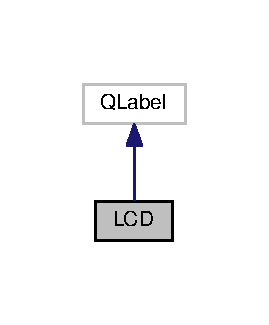
\includegraphics[width=129pt]{class_l_c_d__inherit__graph}
\end{center}
\end{figure}


Collaboration diagram for L\-C\-D\-:
\nopagebreak
\begin{figure}[H]
\begin{center}
\leavevmode
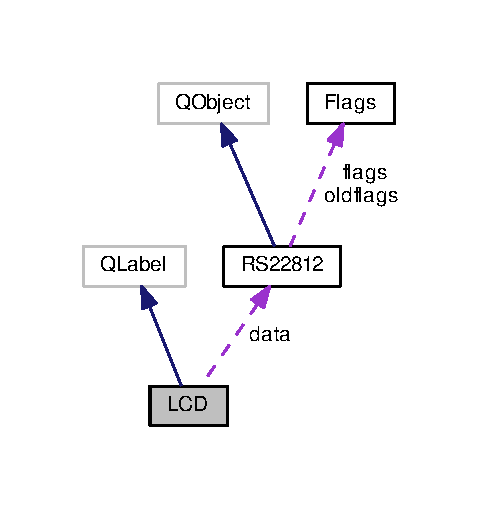
\includegraphics[width=233pt]{class_l_c_d__coll__graph}
\end{center}
\end{figure}
\subsection*{Public Member Functions}
\begin{DoxyCompactItemize}
\item 
\hyperlink{class_l_c_d_a525b305d4aaf0d45cfd04b9b16096482}{L\-C\-D} (const \hyperlink{class_r_s22812}{R\-S22812} $\ast$\hyperlink{class_l_c_d_a04c1fe4d60f692978d1d428521e2d2a2}{data}, Q\-Widget $\ast$parent=0)
\begin{DoxyCompactList}\small\item\em \hyperlink{class_l_c_d_a525b305d4aaf0d45cfd04b9b16096482}{L\-C\-D\-::\-L\-C\-D}. Constructor. \end{DoxyCompactList}\end{DoxyCompactItemize}
\subsection*{Protected Member Functions}
\begin{DoxyCompactItemize}
\item 
void \hyperlink{class_l_c_d_a259fac152add9afdeb4543af4998d14b}{paint\-Event} (Q\-Paint\-Event $\ast$event)
\begin{DoxyCompactList}\small\item\em \hyperlink{class_l_c_d_a259fac152add9afdeb4543af4998d14b}{L\-C\-D\-::paint\-Event}. Paint event handler. \end{DoxyCompactList}\end{DoxyCompactItemize}
\subsection*{Private Attributes}
\begin{DoxyCompactItemize}
\item 
const Q\-Vector$<$ Q\-String $>$ \hyperlink{class_l_c_d_a80e55f48f0e7c7b791fe1602640f708a}{lbl} =\{\char`\"{}Auto\char`\"{},\char`\"{}R\-S232\char`\"{},\char`\"{}Hold\char`\"{},\char`\"{}Rel\char`\"{},\char`\"{}M\-A\-X\char`\"{},\char`\"{}M\-I\-N\char`\"{},\char`\"{}h\-F\-E\char`\"{},\char`\"{}d\-Bm\char`\"{},\char`\"{}Cont\char`\"{},\char`\"{}Diode\char`\"{},\char`\"{}\%\char`\"{},\char`\"{}S\char`\"{}\}
\item 
const \hyperlink{class_r_s22812}{R\-S22812} $\ast$ \hyperlink{class_l_c_d_a04c1fe4d60f692978d1d428521e2d2a2}{data}
\end{DoxyCompactItemize}


\subsection{Detailed Description}
The \hyperlink{class_l_c_d}{L\-C\-D} class displays the numerical value read. 

This class will show a representation of the multimeter's display showing the same values that are shown in the multimeter. 

\subsection{Constructor \& Destructor Documentation}
\hypertarget{class_l_c_d_a525b305d4aaf0d45cfd04b9b16096482}{\index{L\-C\-D@{L\-C\-D}!L\-C\-D@{L\-C\-D}}
\index{L\-C\-D@{L\-C\-D}!LCD@{L\-C\-D}}
\subsubsection[{L\-C\-D}]{\setlength{\rightskip}{0pt plus 5cm}L\-C\-D\-::\-L\-C\-D (
\begin{DoxyParamCaption}
\item[{const {\bf R\-S22812} $\ast$}]{data, }
\item[{Q\-Widget $\ast$}]{parent = {\ttfamily 0}}
\end{DoxyParamCaption}
)\hspace{0.3cm}{\ttfamily [explicit]}}}\label{class_l_c_d_a525b305d4aaf0d45cfd04b9b16096482}


\hyperlink{class_l_c_d_a525b305d4aaf0d45cfd04b9b16096482}{L\-C\-D\-::\-L\-C\-D}. Constructor. 

Multimeter G\-U\-I G\-U\-I for the R\-S-\/232 mode of the Radio Shack 22-\/812. Copyright (C) 2016 F\-J Salguero

This program is free software\-: you can redistribute it and/or modify it under the terms of the G\-N\-U General Public License as published by the Free Software Foundation, either version 3 of the License, or (at your option) any later version.

This program is distributed in the hope that it will be useful, but W\-I\-T\-H\-O\-U\-T A\-N\-Y W\-A\-R\-R\-A\-N\-T\-Y; without even the implied warranty of M\-E\-R\-C\-H\-A\-N\-T\-A\-B\-I\-L\-I\-T\-Y or F\-I\-T\-N\-E\-S\-S F\-O\-R A P\-A\-R\-T\-I\-C\-U\-L\-A\-R P\-U\-R\-P\-O\-S\-E. See the G\-N\-U General Public License for more details.

You should have received a copy of the G\-N\-U General Public License along with this program. If not, see \href{http://www.gnu.org/licenses/}{\tt http\-://www.\-gnu.\-org/licenses/}.


\begin{DoxyParams}{Parameters}
{\em data} & \\
\hline
{\em parent} & \\
\hline
\end{DoxyParams}


\subsection{Member Function Documentation}
\hypertarget{class_l_c_d_a259fac152add9afdeb4543af4998d14b}{\index{L\-C\-D@{L\-C\-D}!paint\-Event@{paint\-Event}}
\index{paint\-Event@{paint\-Event}!LCD@{L\-C\-D}}
\subsubsection[{paint\-Event}]{\setlength{\rightskip}{0pt plus 5cm}void L\-C\-D\-::paint\-Event (
\begin{DoxyParamCaption}
\item[{Q\-Paint\-Event $\ast$}]{event}
\end{DoxyParamCaption}
)\hspace{0.3cm}{\ttfamily [protected]}}}\label{class_l_c_d_a259fac152add9afdeb4543af4998d14b}


\hyperlink{class_l_c_d_a259fac152add9afdeb4543af4998d14b}{L\-C\-D\-::paint\-Event}. Paint event handler. 


\begin{DoxyParams}{Parameters}
{\em event} & It redraws the \hyperlink{class_l_c_d}{L\-C\-D} widget every time there is an update. \\
\hline
\end{DoxyParams}


Here is the call graph for this function\-:\nopagebreak
\begin{figure}[H]
\begin{center}
\leavevmode
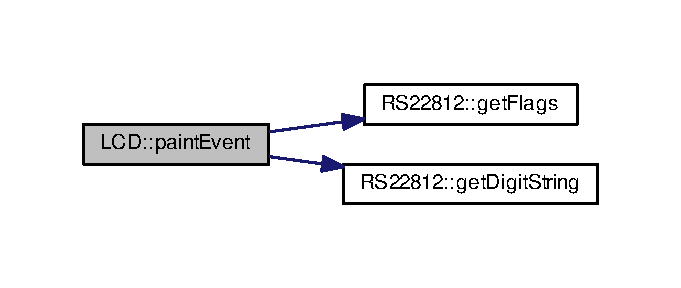
\includegraphics[width=327pt]{class_l_c_d_a259fac152add9afdeb4543af4998d14b_cgraph}
\end{center}
\end{figure}




\subsection{Member Data Documentation}
\hypertarget{class_l_c_d_a04c1fe4d60f692978d1d428521e2d2a2}{\index{L\-C\-D@{L\-C\-D}!data@{data}}
\index{data@{data}!LCD@{L\-C\-D}}
\subsubsection[{data}]{\setlength{\rightskip}{0pt plus 5cm}const {\bf R\-S22812}$\ast$ L\-C\-D\-::data\hspace{0.3cm}{\ttfamily [private]}}}\label{class_l_c_d_a04c1fe4d60f692978d1d428521e2d2a2}
\hypertarget{class_l_c_d_a80e55f48f0e7c7b791fe1602640f708a}{\index{L\-C\-D@{L\-C\-D}!lbl@{lbl}}
\index{lbl@{lbl}!LCD@{L\-C\-D}}
\subsubsection[{lbl}]{\setlength{\rightskip}{0pt plus 5cm}const Q\-Vector$<$Q\-String$>$ L\-C\-D\-::lbl =\{\char`\"{}Auto\char`\"{},\char`\"{}R\-S232\char`\"{},\char`\"{}Hold\char`\"{},\char`\"{}Rel\char`\"{},\char`\"{}M\-A\-X\char`\"{},\char`\"{}M\-I\-N\char`\"{},\char`\"{}h\-F\-E\char`\"{},\char`\"{}d\-Bm\char`\"{},\char`\"{}Cont\char`\"{},\char`\"{}Diode\char`\"{},\char`\"{}\%\char`\"{},\char`\"{}S\char`\"{}\}\hspace{0.3cm}{\ttfamily [private]}}}\label{class_l_c_d_a80e55f48f0e7c7b791fe1602640f708a}


The documentation for this class was generated from the following files\-:\begin{DoxyCompactItemize}
\item 
\hyperlink{lcd_8h}{lcd.\-h}\item 
\hyperlink{lcd_8cpp}{lcd.\-cpp}\end{DoxyCompactItemize}

\hypertarget{class_ui_1_1_main_window}{\section{Ui\-:\-:Main\-Window Class Reference}
\label{class_ui_1_1_main_window}\index{Ui\-::\-Main\-Window@{Ui\-::\-Main\-Window}}
}


{\ttfamily \#include $<$ui\-\_\-mainwindow.\-h$>$}



Inheritance diagram for Ui\-:\-:Main\-Window\-:\nopagebreak
\begin{figure}[H]
\begin{center}
\leavevmode
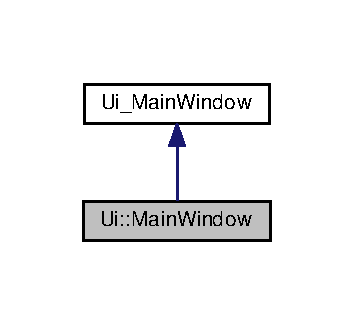
\includegraphics[width=170pt]{class_ui_1_1_main_window__inherit__graph}
\end{center}
\end{figure}


Collaboration diagram for Ui\-:\-:Main\-Window\-:\nopagebreak
\begin{figure}[H]
\begin{center}
\leavevmode
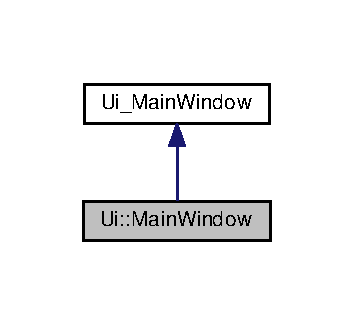
\includegraphics[width=170pt]{class_ui_1_1_main_window__coll__graph}
\end{center}
\end{figure}
\subsection*{Additional Inherited Members}


The documentation for this class was generated from the following file\-:\begin{DoxyCompactItemize}
\item 
build-\/multimeter\-G\-U\-I-\/\-Desktop-\/\-Debug/\hyperlink{ui__mainwindow_8h}{ui\-\_\-mainwindow.\-h}\end{DoxyCompactItemize}

\hypertarget{class_main_window}{\section{Main\-Window Class Reference}
\label{class_main_window}\index{Main\-Window@{Main\-Window}}
}


The \hyperlink{class_main_window}{Main\-Window} class.  




{\ttfamily \#include $<$mainwindow.\-h$>$}



Inheritance diagram for Main\-Window\-:\nopagebreak
\begin{figure}[H]
\begin{center}
\leavevmode
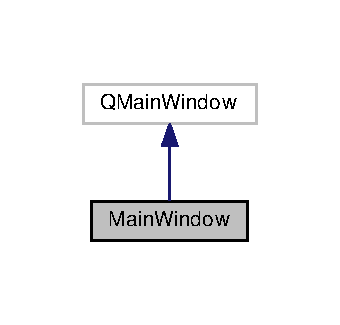
\includegraphics[width=163pt]{class_main_window__inherit__graph}
\end{center}
\end{figure}


Collaboration diagram for Main\-Window\-:\nopagebreak
\begin{figure}[H]
\begin{center}
\leavevmode
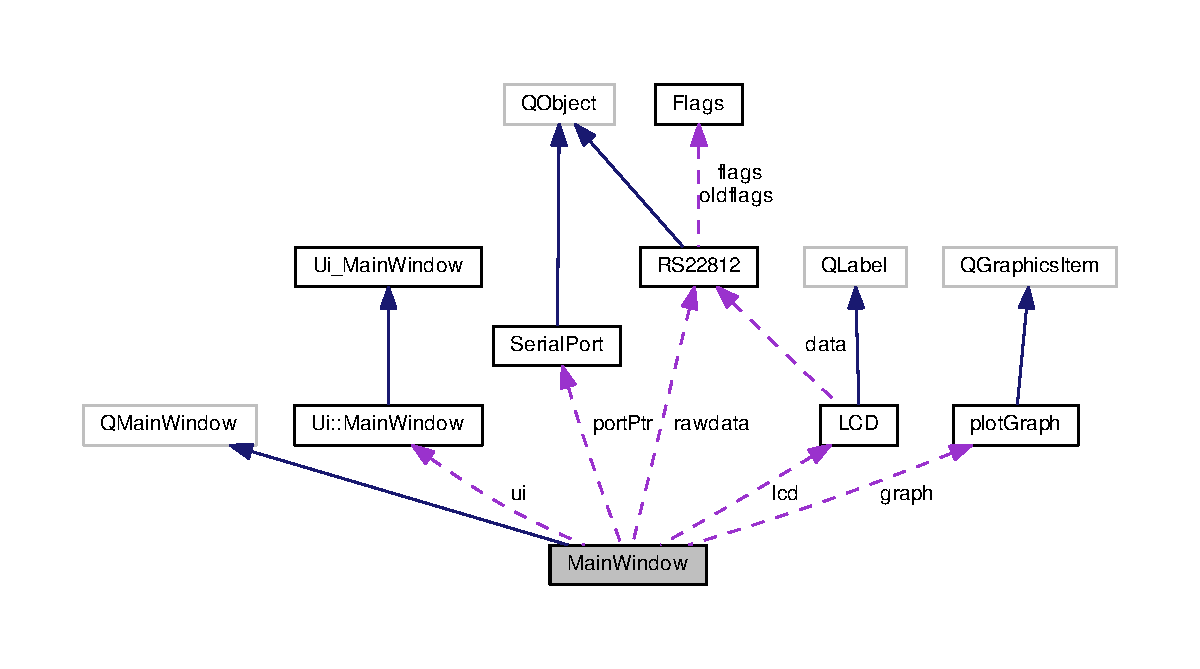
\includegraphics[width=350pt]{class_main_window__coll__graph}
\end{center}
\end{figure}
\subsection*{Public Member Functions}
\begin{DoxyCompactItemize}
\item 
\hyperlink{class_main_window_a8b244be8b7b7db1b08de2a2acb9409db}{Main\-Window} (Q\-Widget $\ast$parent=0)
\begin{DoxyCompactList}\small\item\em Constructor. \end{DoxyCompactList}\item 
\hyperlink{class_main_window_ae98d00a93bc118200eeef9f9bba1dba7}{$\sim$\-Main\-Window} ()
\begin{DoxyCompactList}\small\item\em Destructor. \end{DoxyCompactList}\end{DoxyCompactItemize}
\subsection*{Private Slots}
\begin{DoxyCompactItemize}
\item 
void \hyperlink{class_main_window_a55cd52e7b00aff669290588f8affea5a}{on\-\_\-connect\-Button\-\_\-clicked} ()
\begin{DoxyCompactList}\small\item\em Opens the selected port. \end{DoxyCompactList}\item 
void \hyperlink{class_main_window_ab9336d803a096e94955e032ecf9d0e8b}{on\-\_\-disconnect\-Button\-\_\-clicked} ()
\begin{DoxyCompactList}\small\item\em Disconnect from the current port. \end{DoxyCompactList}\item 
void \hyperlink{class_main_window_a7208eaab614587a945fee7216034aa71}{add\-Data} ()
\begin{DoxyCompactList}\small\item\em Add new data to the data set. This method will be called when new data has been read from the serial port, it will add the new value to the stored set of pairs (time,value) and update the graph. \end{DoxyCompactList}\item 
void \hyperlink{class_main_window_ac9a5649007c5a18e7aa123634866e3a7}{reset\-Data} ()
\begin{DoxyCompactList}\small\item\em Resets the data stored in memory. This method is called when the multimeter's mode changes, clearing all the data stored in memory. \end{DoxyCompactList}\end{DoxyCompactItemize}
\subsection*{Private Attributes}
\begin{DoxyCompactItemize}
\item 
\hyperlink{class_ui_1_1_main_window}{Ui\-::\-Main\-Window} $\ast$ \hyperlink{class_main_window_a35466a70ed47252a0191168126a352a5}{ui}
\item 
\hyperlink{class_serial_port}{Serial\-Port} $\ast$ \hyperlink{class_main_window_ae00babad562899a2cd108ff3ee684990}{port\-Ptr}
\item 
\hyperlink{class_r_s22812}{R\-S22812} $\ast$ \hyperlink{class_main_window_a478554a221305a416f331e9df2569749}{rawdata}
\item 
\hyperlink{class_l_c_d}{L\-C\-D} $\ast$ \hyperlink{class_main_window_a62606e151c6477b9ed1287b792ef2643}{lcd}
\item 
Q\-Label $\ast$ \hyperlink{class_main_window_a89e281849b9cf7d03662402c6bc6012c}{label}
\item 
\hyperlink{classplot_graph}{plot\-Graph} $\ast$ \hyperlink{class_main_window_ac28b469bbf190a49e26ebfb3ff3c8d22}{graph}
\item 
Q\-Graphics\-Scene $\ast$ \hyperlink{class_main_window_a51ac2b126495216832501cea3929c6f6}{scene}
\item 
Q\-Vector$<$ Q\-Pair$<$ qint64, qreal $>$ $>$ \hyperlink{class_main_window_a2759b4057b444152680d6c8ec05a6cac}{store\-Data}
\item 
qint32 \hyperlink{class_main_window_a414ed704b853734bdbde7f0e8e333b20}{counter} =0
\item 
qreal \hyperlink{class_main_window_a02535ba8418420aee9068241aa3e744c}{min\-Data} =99999999
\item 
qreal \hyperlink{class_main_window_a6e7a55c985b905d20ae02cfe0f64d2f2}{max\-Data} =-\/99999999
\item 
Q\-Meta\-Object\-::\-Connection \hyperlink{class_main_window_acff37cb14f3ab80806cc993856632401}{new\-Data}
\item 
Q\-Meta\-Object\-::\-Connection \hyperlink{class_main_window_aa252eef60aa6c3f81a20533a0fe73a2e}{r\-Data}
\item 
Q\-Elapsed\-Timer $\ast$ \hyperlink{class_main_window_a8ce9e134300261f607e1f488a9ef8a1d}{time\-Mark}
\item 
bool \hyperlink{class_main_window_ac5db45f96085abb0a0ac25e981e8d1df}{time\-Running}
\item 
Q\-Vector$<$ Q\-Pair$<$ qreal, qreal $>$ $>$ \hyperlink{class_main_window_a4daf46ba6fc596693c66c97db90cc700}{tmp}
\end{DoxyCompactItemize}


\subsection{Detailed Description}
The \hyperlink{class_main_window}{Main\-Window} class. 

\subsection{Constructor \& Destructor Documentation}
\hypertarget{class_main_window_a8b244be8b7b7db1b08de2a2acb9409db}{\index{Main\-Window@{Main\-Window}!Main\-Window@{Main\-Window}}
\index{Main\-Window@{Main\-Window}!MainWindow@{Main\-Window}}
\subsubsection[{Main\-Window}]{\setlength{\rightskip}{0pt plus 5cm}Main\-Window\-::\-Main\-Window (
\begin{DoxyParamCaption}
\item[{Q\-Widget $\ast$}]{parent = {\ttfamily 0}}
\end{DoxyParamCaption}
)\hspace{0.3cm}{\ttfamily [explicit]}}}\label{class_main_window_a8b244be8b7b7db1b08de2a2acb9409db}


Constructor. 


\begin{DoxyParams}{Parameters}
{\em parent} & The main window constructor will, in addition to create the corresponding subwidgets, populate the list of available ports and connect signals with slots. \\
\hline
\end{DoxyParams}
\begin{DoxyRefDesc}{Todo}
\item[\hyperlink{todo__todo000002}{Todo}]\-: Temporary. It has to be set automatically. \end{DoxyRefDesc}


Here is the call graph for this function\-:
\nopagebreak
\begin{figure}[H]
\begin{center}
\leavevmode
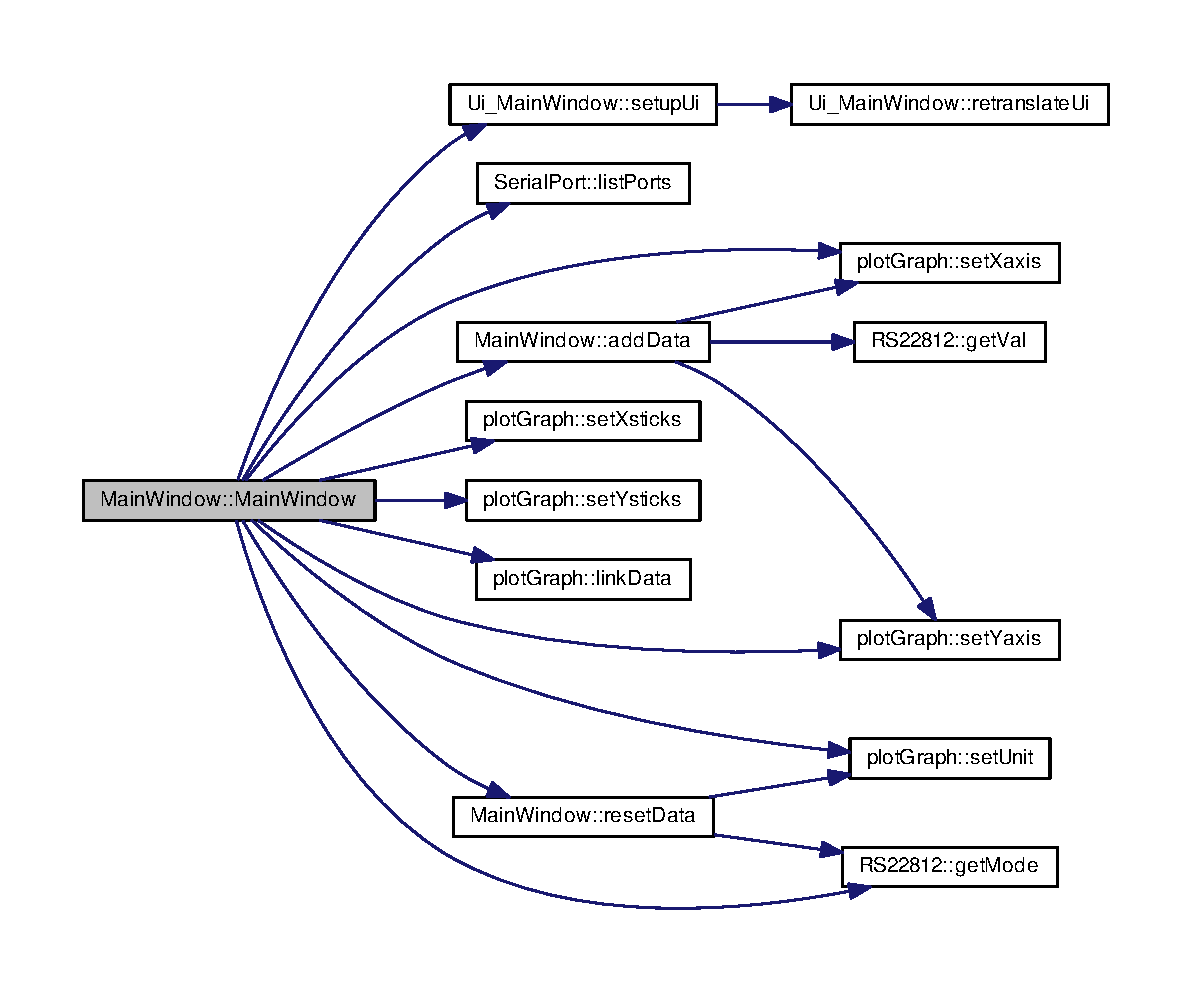
\includegraphics[width=350pt]{class_main_window_a8b244be8b7b7db1b08de2a2acb9409db_cgraph}
\end{center}
\end{figure}


\hypertarget{class_main_window_ae98d00a93bc118200eeef9f9bba1dba7}{\index{Main\-Window@{Main\-Window}!$\sim$\-Main\-Window@{$\sim$\-Main\-Window}}
\index{$\sim$\-Main\-Window@{$\sim$\-Main\-Window}!MainWindow@{Main\-Window}}
\subsubsection[{$\sim$\-Main\-Window}]{\setlength{\rightskip}{0pt plus 5cm}Main\-Window\-::$\sim$\-Main\-Window (
\begin{DoxyParamCaption}
{}
\end{DoxyParamCaption}
)}}\label{class_main_window_ae98d00a93bc118200eeef9f9bba1dba7}


Destructor. 



\subsection{Member Function Documentation}
\hypertarget{class_main_window_a7208eaab614587a945fee7216034aa71}{\index{Main\-Window@{Main\-Window}!add\-Data@{add\-Data}}
\index{add\-Data@{add\-Data}!MainWindow@{Main\-Window}}
\subsubsection[{add\-Data}]{\setlength{\rightskip}{0pt plus 5cm}void Main\-Window\-::add\-Data (
\begin{DoxyParamCaption}
{}
\end{DoxyParamCaption}
)\hspace{0.3cm}{\ttfamily [private]}, {\ttfamily [slot]}}}\label{class_main_window_a7208eaab614587a945fee7216034aa71}


Add new data to the data set. This method will be called when new data has been read from the serial port, it will add the new value to the stored set of pairs (time,value) and update the graph. 



Here is the call graph for this function\-:
\nopagebreak
\begin{figure}[H]
\begin{center}
\leavevmode
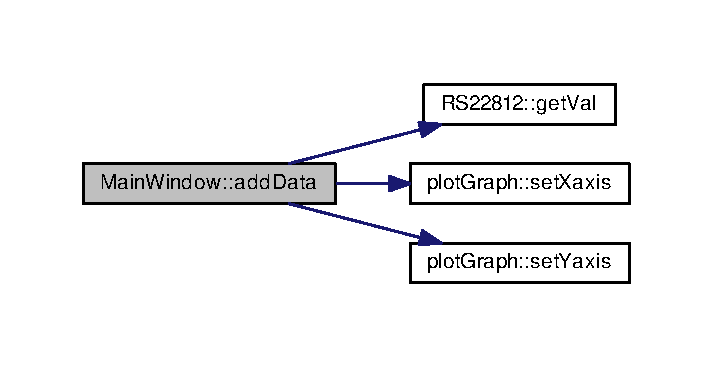
\includegraphics[width=342pt]{class_main_window_a7208eaab614587a945fee7216034aa71_cgraph}
\end{center}
\end{figure}




Here is the caller graph for this function\-:
\nopagebreak
\begin{figure}[H]
\begin{center}
\leavevmode
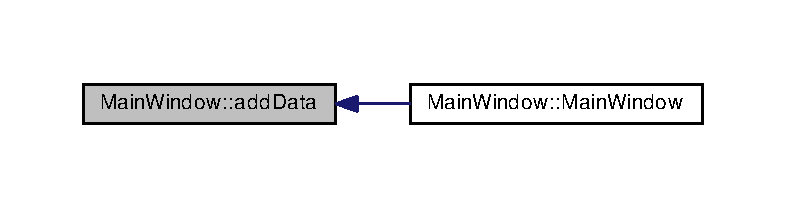
\includegraphics[width=350pt]{class_main_window_a7208eaab614587a945fee7216034aa71_icgraph}
\end{center}
\end{figure}


\hypertarget{class_main_window_a55cd52e7b00aff669290588f8affea5a}{\index{Main\-Window@{Main\-Window}!on\-\_\-connect\-Button\-\_\-clicked@{on\-\_\-connect\-Button\-\_\-clicked}}
\index{on\-\_\-connect\-Button\-\_\-clicked@{on\-\_\-connect\-Button\-\_\-clicked}!MainWindow@{Main\-Window}}
\subsubsection[{on\-\_\-connect\-Button\-\_\-clicked}]{\setlength{\rightskip}{0pt plus 5cm}void Main\-Window\-::on\-\_\-connect\-Button\-\_\-clicked (
\begin{DoxyParamCaption}
{}
\end{DoxyParamCaption}
)\hspace{0.3cm}{\ttfamily [private]}, {\ttfamily [slot]}}}\label{class_main_window_a55cd52e7b00aff669290588f8affea5a}


Opens the selected port. 



Here is the call graph for this function\-:
\nopagebreak
\begin{figure}[H]
\begin{center}
\leavevmode
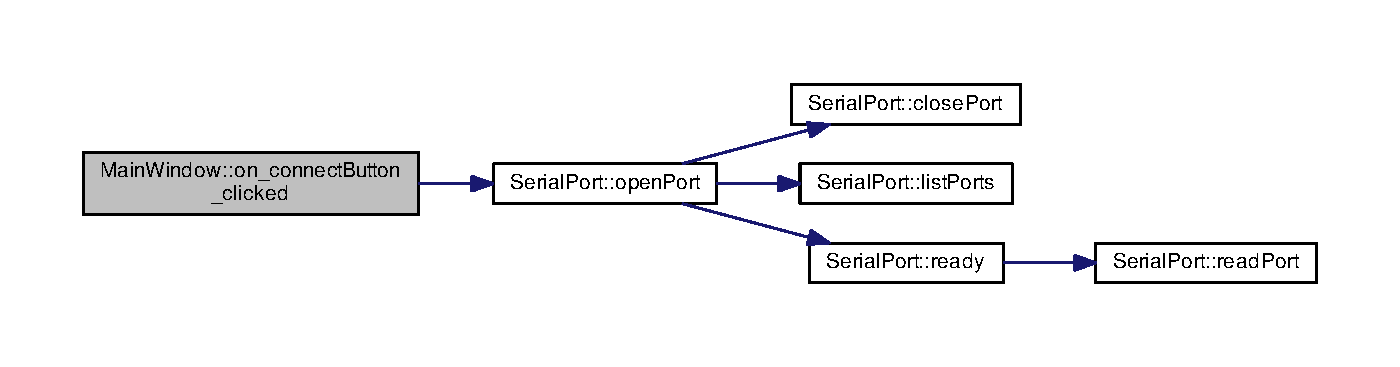
\includegraphics[width=350pt]{class_main_window_a55cd52e7b00aff669290588f8affea5a_cgraph}
\end{center}
\end{figure}


\hypertarget{class_main_window_ab9336d803a096e94955e032ecf9d0e8b}{\index{Main\-Window@{Main\-Window}!on\-\_\-disconnect\-Button\-\_\-clicked@{on\-\_\-disconnect\-Button\-\_\-clicked}}
\index{on\-\_\-disconnect\-Button\-\_\-clicked@{on\-\_\-disconnect\-Button\-\_\-clicked}!MainWindow@{Main\-Window}}
\subsubsection[{on\-\_\-disconnect\-Button\-\_\-clicked}]{\setlength{\rightskip}{0pt plus 5cm}void Main\-Window\-::on\-\_\-disconnect\-Button\-\_\-clicked (
\begin{DoxyParamCaption}
{}
\end{DoxyParamCaption}
)\hspace{0.3cm}{\ttfamily [private]}, {\ttfamily [slot]}}}\label{class_main_window_ab9336d803a096e94955e032ecf9d0e8b}


Disconnect from the current port. 



Here is the call graph for this function\-:
\nopagebreak
\begin{figure}[H]
\begin{center}
\leavevmode
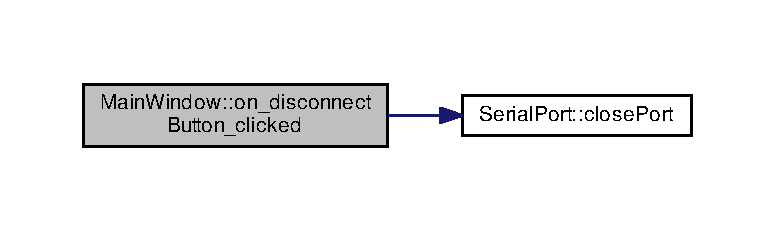
\includegraphics[width=350pt]{class_main_window_ab9336d803a096e94955e032ecf9d0e8b_cgraph}
\end{center}
\end{figure}


\hypertarget{class_main_window_ac9a5649007c5a18e7aa123634866e3a7}{\index{Main\-Window@{Main\-Window}!reset\-Data@{reset\-Data}}
\index{reset\-Data@{reset\-Data}!MainWindow@{Main\-Window}}
\subsubsection[{reset\-Data}]{\setlength{\rightskip}{0pt plus 5cm}void Main\-Window\-::reset\-Data (
\begin{DoxyParamCaption}
{}
\end{DoxyParamCaption}
)\hspace{0.3cm}{\ttfamily [private]}, {\ttfamily [slot]}}}\label{class_main_window_ac9a5649007c5a18e7aa123634866e3a7}


Resets the data stored in memory. This method is called when the multimeter's mode changes, clearing all the data stored in memory. 



Here is the call graph for this function\-:
\nopagebreak
\begin{figure}[H]
\begin{center}
\leavevmode
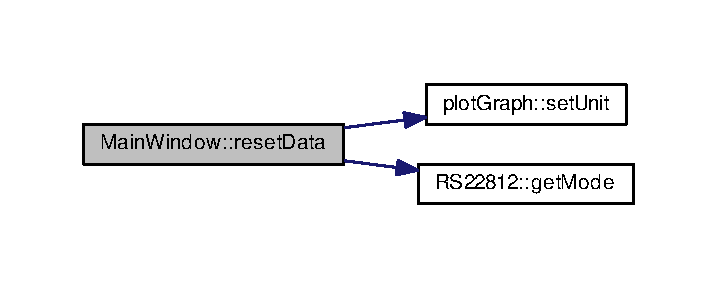
\includegraphics[width=344pt]{class_main_window_ac9a5649007c5a18e7aa123634866e3a7_cgraph}
\end{center}
\end{figure}




Here is the caller graph for this function\-:
\nopagebreak
\begin{figure}[H]
\begin{center}
\leavevmode
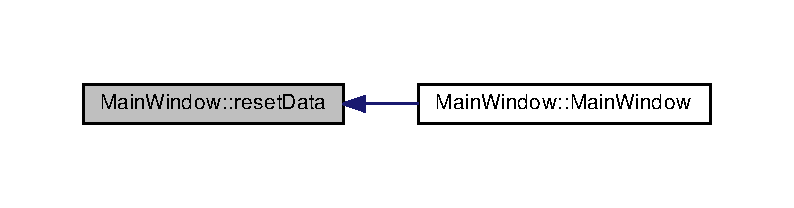
\includegraphics[width=350pt]{class_main_window_ac9a5649007c5a18e7aa123634866e3a7_icgraph}
\end{center}
\end{figure}




\subsection{Member Data Documentation}
\hypertarget{class_main_window_a414ed704b853734bdbde7f0e8e333b20}{\index{Main\-Window@{Main\-Window}!counter@{counter}}
\index{counter@{counter}!MainWindow@{Main\-Window}}
\subsubsection[{counter}]{\setlength{\rightskip}{0pt plus 5cm}qint32 Main\-Window\-::counter =0\hspace{0.3cm}{\ttfamily [private]}}}\label{class_main_window_a414ed704b853734bdbde7f0e8e333b20}
\hypertarget{class_main_window_ac28b469bbf190a49e26ebfb3ff3c8d22}{\index{Main\-Window@{Main\-Window}!graph@{graph}}
\index{graph@{graph}!MainWindow@{Main\-Window}}
\subsubsection[{graph}]{\setlength{\rightskip}{0pt plus 5cm}{\bf plot\-Graph}$\ast$ Main\-Window\-::graph\hspace{0.3cm}{\ttfamily [private]}}}\label{class_main_window_ac28b469bbf190a49e26ebfb3ff3c8d22}
\hypertarget{class_main_window_a89e281849b9cf7d03662402c6bc6012c}{\index{Main\-Window@{Main\-Window}!label@{label}}
\index{label@{label}!MainWindow@{Main\-Window}}
\subsubsection[{label}]{\setlength{\rightskip}{0pt plus 5cm}Q\-Label$\ast$ Main\-Window\-::label\hspace{0.3cm}{\ttfamily [private]}}}\label{class_main_window_a89e281849b9cf7d03662402c6bc6012c}
\hypertarget{class_main_window_a62606e151c6477b9ed1287b792ef2643}{\index{Main\-Window@{Main\-Window}!lcd@{lcd}}
\index{lcd@{lcd}!MainWindow@{Main\-Window}}
\subsubsection[{lcd}]{\setlength{\rightskip}{0pt plus 5cm}{\bf L\-C\-D}$\ast$ Main\-Window\-::lcd\hspace{0.3cm}{\ttfamily [private]}}}\label{class_main_window_a62606e151c6477b9ed1287b792ef2643}
\hypertarget{class_main_window_a6e7a55c985b905d20ae02cfe0f64d2f2}{\index{Main\-Window@{Main\-Window}!max\-Data@{max\-Data}}
\index{max\-Data@{max\-Data}!MainWindow@{Main\-Window}}
\subsubsection[{max\-Data}]{\setlength{\rightskip}{0pt plus 5cm}qreal Main\-Window\-::max\-Data =-\/99999999\hspace{0.3cm}{\ttfamily [private]}}}\label{class_main_window_a6e7a55c985b905d20ae02cfe0f64d2f2}
\hypertarget{class_main_window_a02535ba8418420aee9068241aa3e744c}{\index{Main\-Window@{Main\-Window}!min\-Data@{min\-Data}}
\index{min\-Data@{min\-Data}!MainWindow@{Main\-Window}}
\subsubsection[{min\-Data}]{\setlength{\rightskip}{0pt plus 5cm}qreal Main\-Window\-::min\-Data =99999999\hspace{0.3cm}{\ttfamily [private]}}}\label{class_main_window_a02535ba8418420aee9068241aa3e744c}
\hypertarget{class_main_window_acff37cb14f3ab80806cc993856632401}{\index{Main\-Window@{Main\-Window}!new\-Data@{new\-Data}}
\index{new\-Data@{new\-Data}!MainWindow@{Main\-Window}}
\subsubsection[{new\-Data}]{\setlength{\rightskip}{0pt plus 5cm}Q\-Meta\-Object\-::\-Connection Main\-Window\-::new\-Data\hspace{0.3cm}{\ttfamily [private]}}}\label{class_main_window_acff37cb14f3ab80806cc993856632401}
\hypertarget{class_main_window_ae00babad562899a2cd108ff3ee684990}{\index{Main\-Window@{Main\-Window}!port\-Ptr@{port\-Ptr}}
\index{port\-Ptr@{port\-Ptr}!MainWindow@{Main\-Window}}
\subsubsection[{port\-Ptr}]{\setlength{\rightskip}{0pt plus 5cm}{\bf Serial\-Port}$\ast$ Main\-Window\-::port\-Ptr\hspace{0.3cm}{\ttfamily [private]}}}\label{class_main_window_ae00babad562899a2cd108ff3ee684990}
\hypertarget{class_main_window_a478554a221305a416f331e9df2569749}{\index{Main\-Window@{Main\-Window}!rawdata@{rawdata}}
\index{rawdata@{rawdata}!MainWindow@{Main\-Window}}
\subsubsection[{rawdata}]{\setlength{\rightskip}{0pt plus 5cm}{\bf R\-S22812}$\ast$ Main\-Window\-::rawdata\hspace{0.3cm}{\ttfamily [private]}}}\label{class_main_window_a478554a221305a416f331e9df2569749}
\hypertarget{class_main_window_aa252eef60aa6c3f81a20533a0fe73a2e}{\index{Main\-Window@{Main\-Window}!r\-Data@{r\-Data}}
\index{r\-Data@{r\-Data}!MainWindow@{Main\-Window}}
\subsubsection[{r\-Data}]{\setlength{\rightskip}{0pt plus 5cm}Q\-Meta\-Object\-::\-Connection Main\-Window\-::r\-Data\hspace{0.3cm}{\ttfamily [private]}}}\label{class_main_window_aa252eef60aa6c3f81a20533a0fe73a2e}
\hypertarget{class_main_window_a51ac2b126495216832501cea3929c6f6}{\index{Main\-Window@{Main\-Window}!scene@{scene}}
\index{scene@{scene}!MainWindow@{Main\-Window}}
\subsubsection[{scene}]{\setlength{\rightskip}{0pt plus 5cm}Q\-Graphics\-Scene$\ast$ Main\-Window\-::scene\hspace{0.3cm}{\ttfamily [private]}}}\label{class_main_window_a51ac2b126495216832501cea3929c6f6}
\hypertarget{class_main_window_a2759b4057b444152680d6c8ec05a6cac}{\index{Main\-Window@{Main\-Window}!store\-Data@{store\-Data}}
\index{store\-Data@{store\-Data}!MainWindow@{Main\-Window}}
\subsubsection[{store\-Data}]{\setlength{\rightskip}{0pt plus 5cm}Q\-Vector$<$Q\-Pair$<$qint64,qreal$>$ $>$ Main\-Window\-::store\-Data\hspace{0.3cm}{\ttfamily [private]}}}\label{class_main_window_a2759b4057b444152680d6c8ec05a6cac}
\hypertarget{class_main_window_a8ce9e134300261f607e1f488a9ef8a1d}{\index{Main\-Window@{Main\-Window}!time\-Mark@{time\-Mark}}
\index{time\-Mark@{time\-Mark}!MainWindow@{Main\-Window}}
\subsubsection[{time\-Mark}]{\setlength{\rightskip}{0pt plus 5cm}Q\-Elapsed\-Timer$\ast$ Main\-Window\-::time\-Mark\hspace{0.3cm}{\ttfamily [private]}}}\label{class_main_window_a8ce9e134300261f607e1f488a9ef8a1d}
\hypertarget{class_main_window_ac5db45f96085abb0a0ac25e981e8d1df}{\index{Main\-Window@{Main\-Window}!time\-Running@{time\-Running}}
\index{time\-Running@{time\-Running}!MainWindow@{Main\-Window}}
\subsubsection[{time\-Running}]{\setlength{\rightskip}{0pt plus 5cm}bool Main\-Window\-::time\-Running\hspace{0.3cm}{\ttfamily [private]}}}\label{class_main_window_ac5db45f96085abb0a0ac25e981e8d1df}
\hypertarget{class_main_window_a4daf46ba6fc596693c66c97db90cc700}{\index{Main\-Window@{Main\-Window}!tmp@{tmp}}
\index{tmp@{tmp}!MainWindow@{Main\-Window}}
\subsubsection[{tmp}]{\setlength{\rightskip}{0pt plus 5cm}Q\-Vector$<$Q\-Pair$<$qreal,qreal$>$ $>$ Main\-Window\-::tmp\hspace{0.3cm}{\ttfamily [private]}}}\label{class_main_window_a4daf46ba6fc596693c66c97db90cc700}
\hypertarget{class_main_window_a35466a70ed47252a0191168126a352a5}{\index{Main\-Window@{Main\-Window}!ui@{ui}}
\index{ui@{ui}!MainWindow@{Main\-Window}}
\subsubsection[{ui}]{\setlength{\rightskip}{0pt plus 5cm}{\bf Ui\-::\-Main\-Window}$\ast$ Main\-Window\-::ui\hspace{0.3cm}{\ttfamily [private]}}}\label{class_main_window_a35466a70ed47252a0191168126a352a5}


The documentation for this class was generated from the following files\-:\begin{DoxyCompactItemize}
\item 
\hyperlink{mainwindow_8h}{mainwindow.\-h}\item 
\hyperlink{mainwindow_8cpp}{mainwindow.\-cpp}\end{DoxyCompactItemize}

\hypertarget{classplot_graph}{\section{plot\-Graph Class Reference}
\label{classplot_graph}\index{plot\-Graph@{plot\-Graph}}
}


The \hyperlink{classplot_graph}{plot\-Graph} class.  




{\ttfamily \#include $<$plotgraph.\-h$>$}



Inheritance diagram for plot\-Graph\-:\nopagebreak
\begin{figure}[H]
\begin{center}
\leavevmode
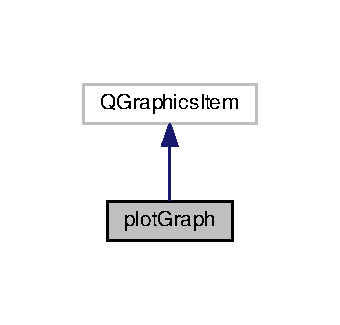
\includegraphics[width=163pt]{classplot_graph__inherit__graph}
\end{center}
\end{figure}


Collaboration diagram for plot\-Graph\-:\nopagebreak
\begin{figure}[H]
\begin{center}
\leavevmode
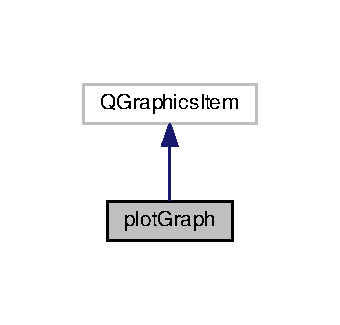
\includegraphics[width=163pt]{classplot_graph__coll__graph}
\end{center}
\end{figure}
\subsection*{Public Member Functions}
\begin{DoxyCompactItemize}
\item 
\hyperlink{classplot_graph_a53902ce2d9f08bfda697a887061b12ca}{plot\-Graph} ()
\begin{DoxyCompactList}\small\item\em \hyperlink{classplot_graph}{plot\-Graph}. Default constructor. \end{DoxyCompactList}\item 
\hyperlink{classplot_graph_ad42c2f82cf414d72aec713f03e1cba0e}{plot\-Graph} (Q\-Graphics\-Scene $\ast$\-\_\-scene)
\begin{DoxyCompactList}\small\item\em \hyperlink{classplot_graph}{plot\-Graph}. Constructor. \end{DoxyCompactList}\item 
void \hyperlink{classplot_graph_aa72b60c4f95834599921874fab85d01b}{paint} (Q\-Painter $\ast$painter, const Q\-Style\-Option\-Graphics\-Item $\ast$option, Q\-Widget $\ast$widget)
\begin{DoxyCompactList}\small\item\em Override of the paint method of Q\-Graphics\-Scene. \end{DoxyCompactList}\item 
Q\-Rect\-F \hyperlink{classplot_graph_a65061b6dda44811830977d80f46ed15e}{bounding\-Rect} () const 
\begin{DoxyCompactList}\small\item\em Returns the bounding rectangle of the graph. \end{DoxyCompactList}\item 
void \hyperlink{classplot_graph_a860f6e766de63d3a7a251f528dcc4be7}{set\-Xaxis} (qint64 min\-Val, qint64 max\-Val)
\begin{DoxyCompactList}\small\item\em Sets the maximum and minimum values of the x axis. \end{DoxyCompactList}\item 
void \hyperlink{classplot_graph_a0e2e3589bfc5cc726e367bf8bdc8a2f5}{set\-Yaxis} (qreal min\-Val, qreal max\-Val)
\begin{DoxyCompactList}\small\item\em Sets the maximum and minimum values of the y axis. \end{DoxyCompactList}\item 
void \hyperlink{classplot_graph_ab78b439ee76e1f4df9a9e26ebcd3bc29}{set\-Xsticks} (int n\-Sticks)
\begin{DoxyCompactList}\small\item\em Sets the number of sticks in the x axis. \end{DoxyCompactList}\item 
void \hyperlink{classplot_graph_af5944ac87c177035eeeaf61d64b1a139}{set\-Ysticks} (int n\-Sticks)
\begin{DoxyCompactList}\small\item\em Sets the number of sticks in the y axis. \end{DoxyCompactList}\item 
void \hyperlink{classplot_graph_a8eb89c53d633e0a9574f1670c9c0d644}{link\-Data} (const Q\-Vector$<$ Q\-Pair$<$ qint64, qreal $>$ $>$ $\ast$dat)
\begin{DoxyCompactList}\small\item\em Links the data being plotted with the data vector that is being acquired from the port. \end{DoxyCompactList}\item 
void \hyperlink{classplot_graph_a09a7563bcd8a387e1d9bf3f534ecd990}{set\-Unit} (int U)
\begin{DoxyCompactList}\small\item\em Selects the appropriate unit depending on the multimeter setting. \end{DoxyCompactList}\item 
void \hyperlink{classplot_graph_ace55db051cab85e9a0c20795f4c2349a}{set\-Scene} (Q\-Graphics\-Scene $\ast$\hyperlink{classplot_graph_ac35eabe1a0ffbb4379fedebe6d5057c3}{scene})
\end{DoxyCompactItemize}
\subsection*{Private Member Functions}
\begin{DoxyCompactItemize}
\item 
void \hyperlink{classplot_graph_a9237c8835c854dfe3156d4a5803663ab}{paint\-Axis} (Q\-Painter $\ast$painter, const Q\-Style\-Option\-Graphics\-Item $\ast$option, Q\-Widget $\ast$widget)
\begin{DoxyCompactList}\small\item\em Calculates the scale and limits of the axis and draws it. \end{DoxyCompactList}\item 
void \hyperlink{classplot_graph_a15feece3d49379208e40d2cd1b560787}{plot\-Data} (Q\-Painter $\ast$painter, const Q\-Style\-Option\-Graphics\-Item $\ast$option, Q\-Widget $\ast$widget)
\begin{DoxyCompactList}\small\item\em Draws the data on the widget. \end{DoxyCompactList}\item 
void \hyperlink{classplot_graph_aafb4adc423d484284f192dee28b00b8a}{label\-Xaxis} (Q\-Painter $\ast$painter, Q\-Point \&p1, Q\-Point \&p2)
\begin{DoxyCompactList}\small\item\em Adds labels to the X axis. \end{DoxyCompactList}\item 
void \hyperlink{classplot_graph_a101e15e7b8cb1ca251e736777a091ee3}{label\-Yaxis} (Q\-Painter $\ast$painter, Q\-Point \&p1, Q\-Point \&p2)
\begin{DoxyCompactList}\small\item\em Adds labels to the Y axis. \end{DoxyCompactList}\item 
Q\-Point \hyperlink{classplot_graph_afecabc6fb684c043bef8f585eb7e0791}{real2\-Coord} (const Q\-Pair$<$ qreal, qreal $>$ dpoint)
\begin{DoxyCompactList}\small\item\em Transforms reading coordinates to widget coordinates. \end{DoxyCompactList}\end{DoxyCompactItemize}
\subsection*{Private Attributes}
\begin{DoxyCompactItemize}
\item 
Q\-Rect \hyperlink{classplot_graph_a82ade58d0ea960ec8c13bb3e0b084b8a}{b\-Rect} =Q\-Rect(0,0,0,0)
\item 
Q\-Point \hyperlink{classplot_graph_a1d47ee94eb0d3a2894723e4e12765d32}{origin}
\item 
Q\-Point \hyperlink{classplot_graph_a07f4680de55428eb49d593106414ccd9}{right\-X}
\item 
Q\-Point \hyperlink{classplot_graph_a32de5c2ff068bd201bc627eaf2d18322}{upper\-Y}
\item 
const int \hyperlink{classplot_graph_addb0f7d6a06ae97184b3013cccb6f456}{axis\-Margin} =40
\item 
qreal \hyperlink{classplot_graph_a45c23930851a6130acdc537755e467fa}{xmin} =0
\item 
qreal \hyperlink{classplot_graph_ac270a2ae2617fe5554eb99c9ae631f48}{xmax} =1
\item 
qreal \hyperlink{classplot_graph_a5746beef331fbadbf5e1a767b7ed7462}{ymin} =0
\item 
qreal \hyperlink{classplot_graph_a14556cbab64df6e06812a0578041956c}{ymax} =1
\item 
int \hyperlink{classplot_graph_adb0cd0f56da1aa52084da70231c92255}{nx} =2
\item 
int \hyperlink{classplot_graph_a1f6efb75c6de2d3da038666610df3aca}{ny} =2
\item 
const Q\-Vector$<$ Q\-Pair$<$ qint64, \\*
qreal $>$ $>$ $\ast$ \hyperlink{classplot_graph_af219b9987999a1b1c2b9af03a6cb93d1}{data} =N\-U\-L\-L
\item 
Q\-String \hyperlink{classplot_graph_a2e0df5fa1ed5f1448bae3d4404b1a6e5}{unit}
\item 
Q\-Graphics\-Scene $\ast$ \hyperlink{classplot_graph_ac35eabe1a0ffbb4379fedebe6d5057c3}{scene}
\end{DoxyCompactItemize}


\subsection{Detailed Description}
The \hyperlink{classplot_graph}{plot\-Graph} class. 

This class graphs the values read from the multimeter versus the time. 

\subsection{Constructor \& Destructor Documentation}
\hypertarget{classplot_graph_a53902ce2d9f08bfda697a887061b12ca}{\index{plot\-Graph@{plot\-Graph}!plot\-Graph@{plot\-Graph}}
\index{plot\-Graph@{plot\-Graph}!plotGraph@{plot\-Graph}}
\subsubsection[{plot\-Graph}]{\setlength{\rightskip}{0pt plus 5cm}plot\-Graph\-::plot\-Graph (
\begin{DoxyParamCaption}
{}
\end{DoxyParamCaption}
)\hspace{0.3cm}{\ttfamily [inline]}}}\label{classplot_graph_a53902ce2d9f08bfda697a887061b12ca}


\hyperlink{classplot_graph}{plot\-Graph}. Default constructor. 

\hypertarget{classplot_graph_ad42c2f82cf414d72aec713f03e1cba0e}{\index{plot\-Graph@{plot\-Graph}!plot\-Graph@{plot\-Graph}}
\index{plot\-Graph@{plot\-Graph}!plotGraph@{plot\-Graph}}
\subsubsection[{plot\-Graph}]{\setlength{\rightskip}{0pt plus 5cm}plot\-Graph\-::plot\-Graph (
\begin{DoxyParamCaption}
\item[{Q\-Graphics\-Scene $\ast$}]{\-\_\-scene}
\end{DoxyParamCaption}
)\hspace{0.3cm}{\ttfamily [inline]}}}\label{classplot_graph_ad42c2f82cf414d72aec713f03e1cba0e}


\hyperlink{classplot_graph}{plot\-Graph}. Constructor. 


\begin{DoxyParams}{Parameters}
{\em \-\_\-scene} & \\
\hline
\end{DoxyParams}


\subsection{Member Function Documentation}
\hypertarget{classplot_graph_a65061b6dda44811830977d80f46ed15e}{\index{plot\-Graph@{plot\-Graph}!bounding\-Rect@{bounding\-Rect}}
\index{bounding\-Rect@{bounding\-Rect}!plotGraph@{plot\-Graph}}
\subsubsection[{bounding\-Rect}]{\setlength{\rightskip}{0pt plus 5cm}Q\-Rect\-F plot\-Graph\-::bounding\-Rect (
\begin{DoxyParamCaption}
{}
\end{DoxyParamCaption}
) const}}\label{classplot_graph_a65061b6dda44811830977d80f46ed15e}


Returns the bounding rectangle of the graph. 

\begin{DoxyReturn}{Returns}
So far, it returns a fake value. Need to implement. 
\end{DoxyReturn}
\hypertarget{classplot_graph_aafb4adc423d484284f192dee28b00b8a}{\index{plot\-Graph@{plot\-Graph}!label\-Xaxis@{label\-Xaxis}}
\index{label\-Xaxis@{label\-Xaxis}!plotGraph@{plot\-Graph}}
\subsubsection[{label\-Xaxis}]{\setlength{\rightskip}{0pt plus 5cm}void plot\-Graph\-::label\-Xaxis (
\begin{DoxyParamCaption}
\item[{Q\-Painter $\ast$}]{painter, }
\item[{Q\-Point \&}]{p1, }
\item[{Q\-Point \&}]{p2}
\end{DoxyParamCaption}
)\hspace{0.3cm}{\ttfamily [private]}}}\label{classplot_graph_aafb4adc423d484284f192dee28b00b8a}


Adds labels to the X axis. 


\begin{DoxyParams}{Parameters}
{\em painter} & \\
\hline
{\em p1} & \\
\hline
{\em p2} & \\
\hline
\end{DoxyParams}


Here is the caller graph for this function\-:
\nopagebreak
\begin{figure}[H]
\begin{center}
\leavevmode
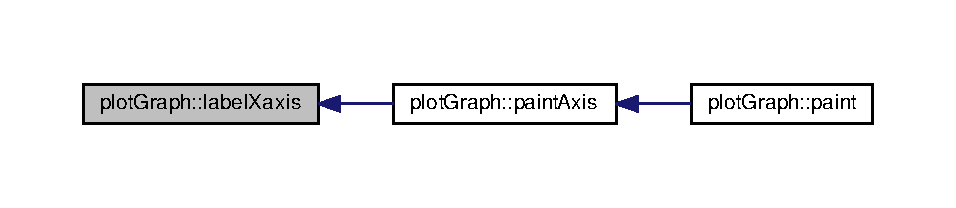
\includegraphics[width=350pt]{classplot_graph_aafb4adc423d484284f192dee28b00b8a_icgraph}
\end{center}
\end{figure}


\hypertarget{classplot_graph_a101e15e7b8cb1ca251e736777a091ee3}{\index{plot\-Graph@{plot\-Graph}!label\-Yaxis@{label\-Yaxis}}
\index{label\-Yaxis@{label\-Yaxis}!plotGraph@{plot\-Graph}}
\subsubsection[{label\-Yaxis}]{\setlength{\rightskip}{0pt plus 5cm}void plot\-Graph\-::label\-Yaxis (
\begin{DoxyParamCaption}
\item[{Q\-Painter $\ast$}]{painter, }
\item[{Q\-Point \&}]{p1, }
\item[{Q\-Point \&}]{p2}
\end{DoxyParamCaption}
)\hspace{0.3cm}{\ttfamily [private]}}}\label{classplot_graph_a101e15e7b8cb1ca251e736777a091ee3}


Adds labels to the Y axis. 


\begin{DoxyParams}{Parameters}
{\em painter} & \\
\hline
{\em p1} & \\
\hline
{\em p2} & \\
\hline
\end{DoxyParams}


Here is the caller graph for this function\-:
\nopagebreak
\begin{figure}[H]
\begin{center}
\leavevmode
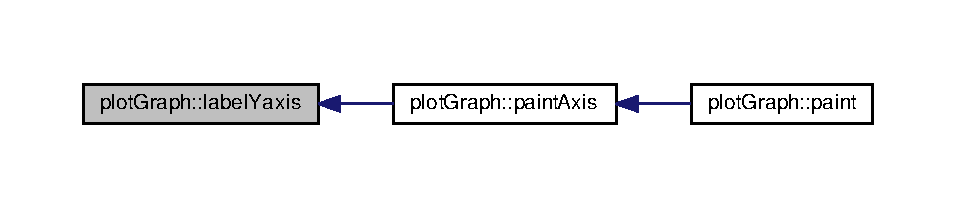
\includegraphics[width=350pt]{classplot_graph_a101e15e7b8cb1ca251e736777a091ee3_icgraph}
\end{center}
\end{figure}


\hypertarget{classplot_graph_a8eb89c53d633e0a9574f1670c9c0d644}{\index{plot\-Graph@{plot\-Graph}!link\-Data@{link\-Data}}
\index{link\-Data@{link\-Data}!plotGraph@{plot\-Graph}}
\subsubsection[{link\-Data}]{\setlength{\rightskip}{0pt plus 5cm}void plot\-Graph\-::link\-Data (
\begin{DoxyParamCaption}
\item[{const Q\-Vector$<$ Q\-Pair$<$ qint64, qreal $>$ $>$ $\ast$}]{dat}
\end{DoxyParamCaption}
)\hspace{0.3cm}{\ttfamily [inline]}}}\label{classplot_graph_a8eb89c53d633e0a9574f1670c9c0d644}


Links the data being plotted with the data vector that is being acquired from the port. 


\begin{DoxyParams}{Parameters}
{\em dat} & \\
\hline
\end{DoxyParams}


Here is the caller graph for this function\-:
\nopagebreak
\begin{figure}[H]
\begin{center}
\leavevmode
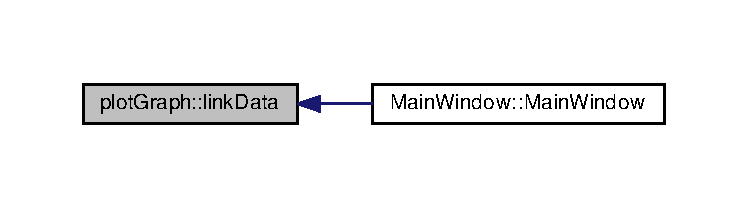
\includegraphics[width=350pt]{classplot_graph_a8eb89c53d633e0a9574f1670c9c0d644_icgraph}
\end{center}
\end{figure}


\hypertarget{classplot_graph_aa72b60c4f95834599921874fab85d01b}{\index{plot\-Graph@{plot\-Graph}!paint@{paint}}
\index{paint@{paint}!plotGraph@{plot\-Graph}}
\subsubsection[{paint}]{\setlength{\rightskip}{0pt plus 5cm}void plot\-Graph\-::paint (
\begin{DoxyParamCaption}
\item[{Q\-Painter $\ast$}]{painter, }
\item[{const Q\-Style\-Option\-Graphics\-Item $\ast$}]{option, }
\item[{Q\-Widget $\ast$}]{widget}
\end{DoxyParamCaption}
)}}\label{classplot_graph_aa72b60c4f95834599921874fab85d01b}


Override of the paint method of Q\-Graphics\-Scene. 


\begin{DoxyParams}{Parameters}
{\em painter} & \\
\hline
{\em option} & \\
\hline
{\em widget} & \\
\hline
\end{DoxyParams}


Here is the call graph for this function\-:
\nopagebreak
\begin{figure}[H]
\begin{center}
\leavevmode
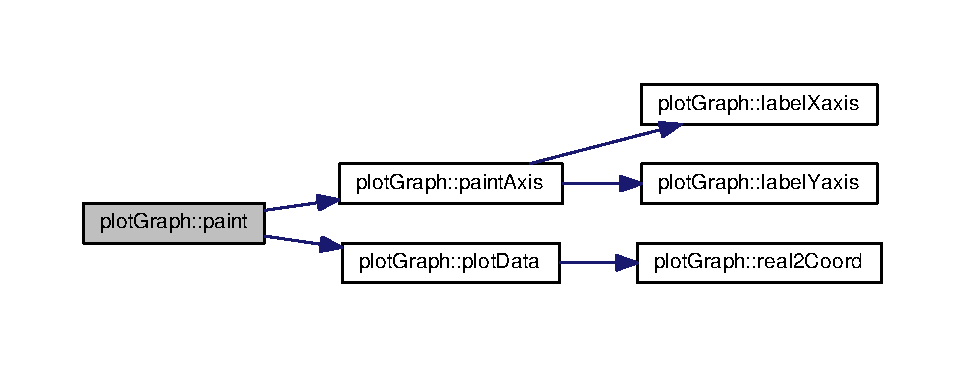
\includegraphics[width=350pt]{classplot_graph_aa72b60c4f95834599921874fab85d01b_cgraph}
\end{center}
\end{figure}


\hypertarget{classplot_graph_a9237c8835c854dfe3156d4a5803663ab}{\index{plot\-Graph@{plot\-Graph}!paint\-Axis@{paint\-Axis}}
\index{paint\-Axis@{paint\-Axis}!plotGraph@{plot\-Graph}}
\subsubsection[{paint\-Axis}]{\setlength{\rightskip}{0pt plus 5cm}void plot\-Graph\-::paint\-Axis (
\begin{DoxyParamCaption}
\item[{Q\-Painter $\ast$}]{painter, }
\item[{const Q\-Style\-Option\-Graphics\-Item $\ast$}]{option, }
\item[{Q\-Widget $\ast$}]{widget}
\end{DoxyParamCaption}
)\hspace{0.3cm}{\ttfamily [private]}}}\label{classplot_graph_a9237c8835c854dfe3156d4a5803663ab}


Calculates the scale and limits of the axis and draws it. 


\begin{DoxyParams}{Parameters}
{\em painter} & \\
\hline
{\em option} & \\
\hline
{\em widget} & \\
\hline
\end{DoxyParams}


Here is the call graph for this function\-:
\nopagebreak
\begin{figure}[H]
\begin{center}
\leavevmode
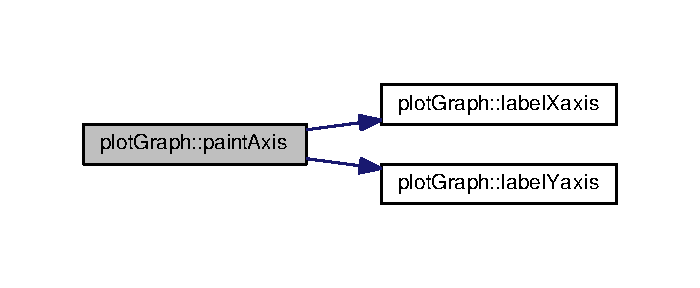
\includegraphics[width=336pt]{classplot_graph_a9237c8835c854dfe3156d4a5803663ab_cgraph}
\end{center}
\end{figure}




Here is the caller graph for this function\-:
\nopagebreak
\begin{figure}[H]
\begin{center}
\leavevmode
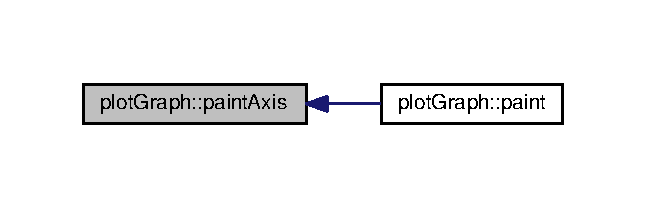
\includegraphics[width=310pt]{classplot_graph_a9237c8835c854dfe3156d4a5803663ab_icgraph}
\end{center}
\end{figure}


\hypertarget{classplot_graph_a15feece3d49379208e40d2cd1b560787}{\index{plot\-Graph@{plot\-Graph}!plot\-Data@{plot\-Data}}
\index{plot\-Data@{plot\-Data}!plotGraph@{plot\-Graph}}
\subsubsection[{plot\-Data}]{\setlength{\rightskip}{0pt plus 5cm}void plot\-Graph\-::plot\-Data (
\begin{DoxyParamCaption}
\item[{Q\-Painter $\ast$}]{painter, }
\item[{const Q\-Style\-Option\-Graphics\-Item $\ast$}]{option, }
\item[{Q\-Widget $\ast$}]{widget}
\end{DoxyParamCaption}
)\hspace{0.3cm}{\ttfamily [private]}}}\label{classplot_graph_a15feece3d49379208e40d2cd1b560787}


Draws the data on the widget. 


\begin{DoxyParams}{Parameters}
{\em painter} & \\
\hline
{\em option} & \\
\hline
{\em widget} & \\
\hline
\end{DoxyParams}


Here is the call graph for this function\-:
\nopagebreak
\begin{figure}[H]
\begin{center}
\leavevmode
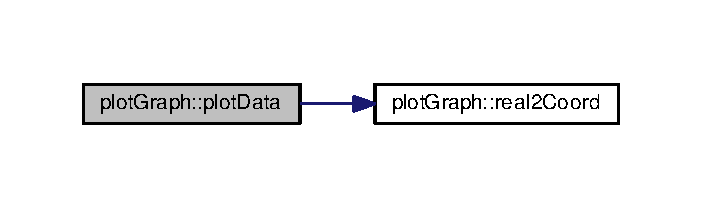
\includegraphics[width=337pt]{classplot_graph_a15feece3d49379208e40d2cd1b560787_cgraph}
\end{center}
\end{figure}




Here is the caller graph for this function\-:
\nopagebreak
\begin{figure}[H]
\begin{center}
\leavevmode
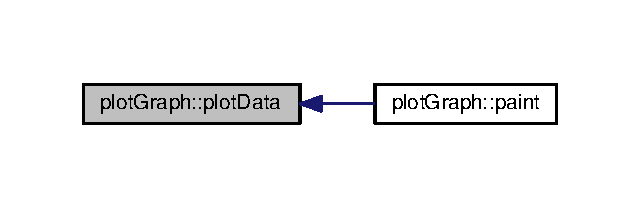
\includegraphics[width=307pt]{classplot_graph_a15feece3d49379208e40d2cd1b560787_icgraph}
\end{center}
\end{figure}


\hypertarget{classplot_graph_afecabc6fb684c043bef8f585eb7e0791}{\index{plot\-Graph@{plot\-Graph}!real2\-Coord@{real2\-Coord}}
\index{real2\-Coord@{real2\-Coord}!plotGraph@{plot\-Graph}}
\subsubsection[{real2\-Coord}]{\setlength{\rightskip}{0pt plus 5cm}Q\-Point plot\-Graph\-::real2\-Coord (
\begin{DoxyParamCaption}
\item[{const Q\-Pair$<$ qreal, qreal $>$}]{dpoint}
\end{DoxyParamCaption}
)\hspace{0.3cm}{\ttfamily [private]}}}\label{classplot_graph_afecabc6fb684c043bef8f585eb7e0791}


Transforms reading coordinates to widget coordinates. 


\begin{DoxyParams}{Parameters}
{\em dpoint} & \\
\hline
\end{DoxyParams}
\begin{DoxyReturn}{Returns}

\end{DoxyReturn}


Here is the caller graph for this function\-:
\nopagebreak
\begin{figure}[H]
\begin{center}
\leavevmode
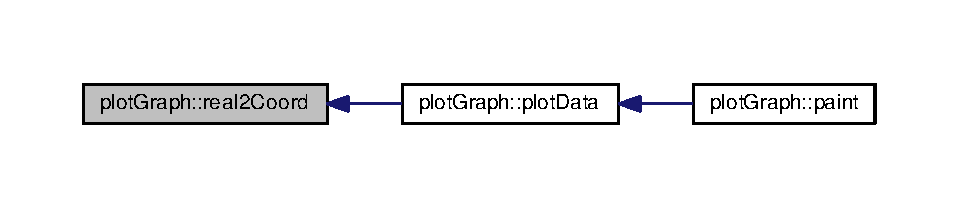
\includegraphics[width=350pt]{classplot_graph_afecabc6fb684c043bef8f585eb7e0791_icgraph}
\end{center}
\end{figure}


\hypertarget{classplot_graph_ace55db051cab85e9a0c20795f4c2349a}{\index{plot\-Graph@{plot\-Graph}!set\-Scene@{set\-Scene}}
\index{set\-Scene@{set\-Scene}!plotGraph@{plot\-Graph}}
\subsubsection[{set\-Scene}]{\setlength{\rightskip}{0pt plus 5cm}void plot\-Graph\-::set\-Scene (
\begin{DoxyParamCaption}
\item[{Q\-Graphics\-Scene $\ast$}]{scene}
\end{DoxyParamCaption}
)}}\label{classplot_graph_ace55db051cab85e9a0c20795f4c2349a}
\hypertarget{classplot_graph_a09a7563bcd8a387e1d9bf3f534ecd990}{\index{plot\-Graph@{plot\-Graph}!set\-Unit@{set\-Unit}}
\index{set\-Unit@{set\-Unit}!plotGraph@{plot\-Graph}}
\subsubsection[{set\-Unit}]{\setlength{\rightskip}{0pt plus 5cm}void plot\-Graph\-::set\-Unit (
\begin{DoxyParamCaption}
\item[{int}]{U}
\end{DoxyParamCaption}
)}}\label{classplot_graph_a09a7563bcd8a387e1d9bf3f534ecd990}


Selects the appropriate unit depending on the multimeter setting. 


\begin{DoxyParams}{Parameters}
{\em U} & \\
\hline
\end{DoxyParams}


Here is the caller graph for this function\-:
\nopagebreak
\begin{figure}[H]
\begin{center}
\leavevmode
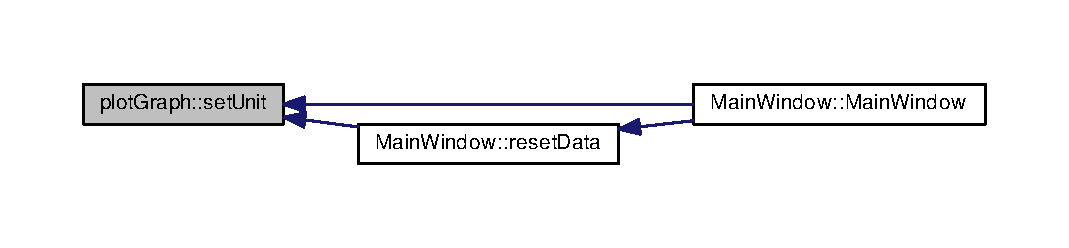
\includegraphics[width=350pt]{classplot_graph_a09a7563bcd8a387e1d9bf3f534ecd990_icgraph}
\end{center}
\end{figure}


\hypertarget{classplot_graph_a860f6e766de63d3a7a251f528dcc4be7}{\index{plot\-Graph@{plot\-Graph}!set\-Xaxis@{set\-Xaxis}}
\index{set\-Xaxis@{set\-Xaxis}!plotGraph@{plot\-Graph}}
\subsubsection[{set\-Xaxis}]{\setlength{\rightskip}{0pt plus 5cm}void plot\-Graph\-::set\-Xaxis (
\begin{DoxyParamCaption}
\item[{qint64}]{min\-Val, }
\item[{qint64}]{max\-Val}
\end{DoxyParamCaption}
)}}\label{classplot_graph_a860f6e766de63d3a7a251f528dcc4be7}


Sets the maximum and minimum values of the x axis. 


\begin{DoxyParams}{Parameters}
{\em min\-Val} & \\
\hline
{\em max\-Val} & \\
\hline
\end{DoxyParams}


Here is the caller graph for this function\-:
\nopagebreak
\begin{figure}[H]
\begin{center}
\leavevmode
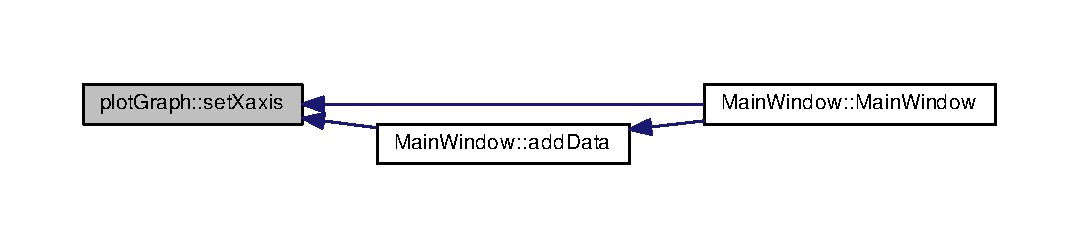
\includegraphics[width=350pt]{classplot_graph_a860f6e766de63d3a7a251f528dcc4be7_icgraph}
\end{center}
\end{figure}


\hypertarget{classplot_graph_ab78b439ee76e1f4df9a9e26ebcd3bc29}{\index{plot\-Graph@{plot\-Graph}!set\-Xsticks@{set\-Xsticks}}
\index{set\-Xsticks@{set\-Xsticks}!plotGraph@{plot\-Graph}}
\subsubsection[{set\-Xsticks}]{\setlength{\rightskip}{0pt plus 5cm}void plot\-Graph\-::set\-Xsticks (
\begin{DoxyParamCaption}
\item[{int}]{n\-Sticks}
\end{DoxyParamCaption}
)\hspace{0.3cm}{\ttfamily [inline]}}}\label{classplot_graph_ab78b439ee76e1f4df9a9e26ebcd3bc29}


Sets the number of sticks in the x axis. 


\begin{DoxyParams}{Parameters}
{\em n\-Sticks} & \\
\hline
\end{DoxyParams}


Here is the caller graph for this function\-:
\nopagebreak
\begin{figure}[H]
\begin{center}
\leavevmode
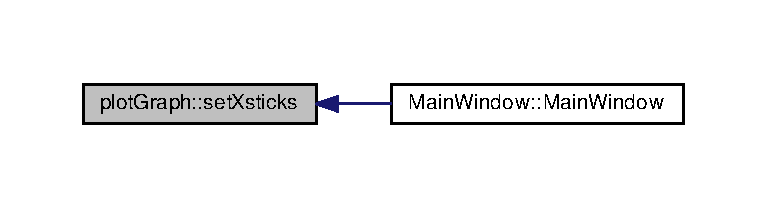
\includegraphics[width=350pt]{classplot_graph_ab78b439ee76e1f4df9a9e26ebcd3bc29_icgraph}
\end{center}
\end{figure}


\hypertarget{classplot_graph_a0e2e3589bfc5cc726e367bf8bdc8a2f5}{\index{plot\-Graph@{plot\-Graph}!set\-Yaxis@{set\-Yaxis}}
\index{set\-Yaxis@{set\-Yaxis}!plotGraph@{plot\-Graph}}
\subsubsection[{set\-Yaxis}]{\setlength{\rightskip}{0pt plus 5cm}void plot\-Graph\-::set\-Yaxis (
\begin{DoxyParamCaption}
\item[{qreal}]{min\-Val, }
\item[{qreal}]{max\-Val}
\end{DoxyParamCaption}
)}}\label{classplot_graph_a0e2e3589bfc5cc726e367bf8bdc8a2f5}


Sets the maximum and minimum values of the y axis. 


\begin{DoxyParams}{Parameters}
{\em min\-Val} & \\
\hline
{\em max\-Val} & \\
\hline
\end{DoxyParams}


Here is the caller graph for this function\-:
\nopagebreak
\begin{figure}[H]
\begin{center}
\leavevmode
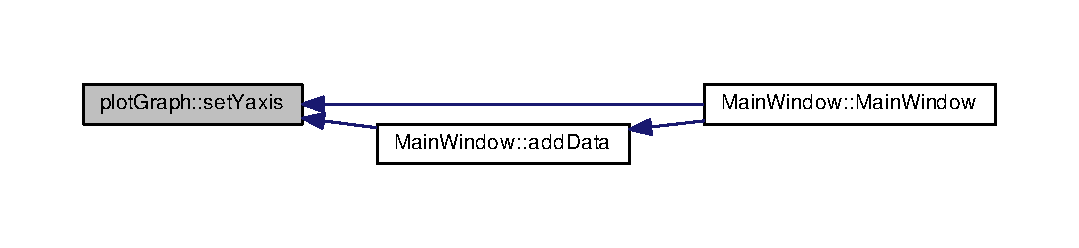
\includegraphics[width=350pt]{classplot_graph_a0e2e3589bfc5cc726e367bf8bdc8a2f5_icgraph}
\end{center}
\end{figure}


\hypertarget{classplot_graph_af5944ac87c177035eeeaf61d64b1a139}{\index{plot\-Graph@{plot\-Graph}!set\-Ysticks@{set\-Ysticks}}
\index{set\-Ysticks@{set\-Ysticks}!plotGraph@{plot\-Graph}}
\subsubsection[{set\-Ysticks}]{\setlength{\rightskip}{0pt plus 5cm}void plot\-Graph\-::set\-Ysticks (
\begin{DoxyParamCaption}
\item[{int}]{n\-Sticks}
\end{DoxyParamCaption}
)\hspace{0.3cm}{\ttfamily [inline]}}}\label{classplot_graph_af5944ac87c177035eeeaf61d64b1a139}


Sets the number of sticks in the y axis. 


\begin{DoxyParams}{Parameters}
{\em n\-Sticks} & \\
\hline
\end{DoxyParams}


Here is the caller graph for this function\-:
\nopagebreak
\begin{figure}[H]
\begin{center}
\leavevmode
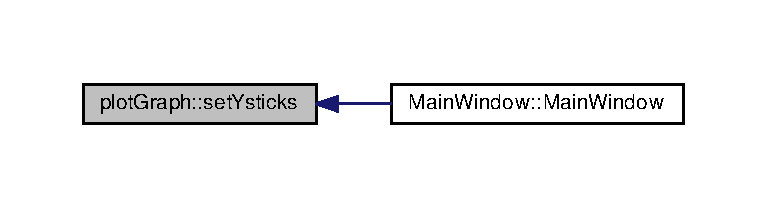
\includegraphics[width=350pt]{classplot_graph_af5944ac87c177035eeeaf61d64b1a139_icgraph}
\end{center}
\end{figure}




\subsection{Member Data Documentation}
\hypertarget{classplot_graph_addb0f7d6a06ae97184b3013cccb6f456}{\index{plot\-Graph@{plot\-Graph}!axis\-Margin@{axis\-Margin}}
\index{axis\-Margin@{axis\-Margin}!plotGraph@{plot\-Graph}}
\subsubsection[{axis\-Margin}]{\setlength{\rightskip}{0pt plus 5cm}const int plot\-Graph\-::axis\-Margin =40\hspace{0.3cm}{\ttfamily [private]}}}\label{classplot_graph_addb0f7d6a06ae97184b3013cccb6f456}
\hypertarget{classplot_graph_a82ade58d0ea960ec8c13bb3e0b084b8a}{\index{plot\-Graph@{plot\-Graph}!b\-Rect@{b\-Rect}}
\index{b\-Rect@{b\-Rect}!plotGraph@{plot\-Graph}}
\subsubsection[{b\-Rect}]{\setlength{\rightskip}{0pt plus 5cm}Q\-Rect plot\-Graph\-::b\-Rect =Q\-Rect(0,0,0,0)\hspace{0.3cm}{\ttfamily [private]}}}\label{classplot_graph_a82ade58d0ea960ec8c13bb3e0b084b8a}
\hypertarget{classplot_graph_af219b9987999a1b1c2b9af03a6cb93d1}{\index{plot\-Graph@{plot\-Graph}!data@{data}}
\index{data@{data}!plotGraph@{plot\-Graph}}
\subsubsection[{data}]{\setlength{\rightskip}{0pt plus 5cm}const Q\-Vector$<$Q\-Pair$<$qint64,qreal$>$ $>$$\ast$ plot\-Graph\-::data =N\-U\-L\-L\hspace{0.3cm}{\ttfamily [private]}}}\label{classplot_graph_af219b9987999a1b1c2b9af03a6cb93d1}
\hypertarget{classplot_graph_adb0cd0f56da1aa52084da70231c92255}{\index{plot\-Graph@{plot\-Graph}!nx@{nx}}
\index{nx@{nx}!plotGraph@{plot\-Graph}}
\subsubsection[{nx}]{\setlength{\rightskip}{0pt plus 5cm}int plot\-Graph\-::nx =2\hspace{0.3cm}{\ttfamily [private]}}}\label{classplot_graph_adb0cd0f56da1aa52084da70231c92255}
\hypertarget{classplot_graph_a1f6efb75c6de2d3da038666610df3aca}{\index{plot\-Graph@{plot\-Graph}!ny@{ny}}
\index{ny@{ny}!plotGraph@{plot\-Graph}}
\subsubsection[{ny}]{\setlength{\rightskip}{0pt plus 5cm}int plot\-Graph\-::ny =2\hspace{0.3cm}{\ttfamily [private]}}}\label{classplot_graph_a1f6efb75c6de2d3da038666610df3aca}
\hypertarget{classplot_graph_a1d47ee94eb0d3a2894723e4e12765d32}{\index{plot\-Graph@{plot\-Graph}!origin@{origin}}
\index{origin@{origin}!plotGraph@{plot\-Graph}}
\subsubsection[{origin}]{\setlength{\rightskip}{0pt plus 5cm}Q\-Point plot\-Graph\-::origin\hspace{0.3cm}{\ttfamily [private]}}}\label{classplot_graph_a1d47ee94eb0d3a2894723e4e12765d32}
\hypertarget{classplot_graph_a07f4680de55428eb49d593106414ccd9}{\index{plot\-Graph@{plot\-Graph}!right\-X@{right\-X}}
\index{right\-X@{right\-X}!plotGraph@{plot\-Graph}}
\subsubsection[{right\-X}]{\setlength{\rightskip}{0pt plus 5cm}Q\-Point plot\-Graph\-::right\-X\hspace{0.3cm}{\ttfamily [private]}}}\label{classplot_graph_a07f4680de55428eb49d593106414ccd9}
\hypertarget{classplot_graph_ac35eabe1a0ffbb4379fedebe6d5057c3}{\index{plot\-Graph@{plot\-Graph}!scene@{scene}}
\index{scene@{scene}!plotGraph@{plot\-Graph}}
\subsubsection[{scene}]{\setlength{\rightskip}{0pt plus 5cm}Q\-Graphics\-Scene$\ast$ plot\-Graph\-::scene\hspace{0.3cm}{\ttfamily [private]}}}\label{classplot_graph_ac35eabe1a0ffbb4379fedebe6d5057c3}
\hypertarget{classplot_graph_a2e0df5fa1ed5f1448bae3d4404b1a6e5}{\index{plot\-Graph@{plot\-Graph}!unit@{unit}}
\index{unit@{unit}!plotGraph@{plot\-Graph}}
\subsubsection[{unit}]{\setlength{\rightskip}{0pt plus 5cm}Q\-String plot\-Graph\-::unit\hspace{0.3cm}{\ttfamily [private]}}}\label{classplot_graph_a2e0df5fa1ed5f1448bae3d4404b1a6e5}
\hypertarget{classplot_graph_a32de5c2ff068bd201bc627eaf2d18322}{\index{plot\-Graph@{plot\-Graph}!upper\-Y@{upper\-Y}}
\index{upper\-Y@{upper\-Y}!plotGraph@{plot\-Graph}}
\subsubsection[{upper\-Y}]{\setlength{\rightskip}{0pt plus 5cm}Q\-Point plot\-Graph\-::upper\-Y\hspace{0.3cm}{\ttfamily [private]}}}\label{classplot_graph_a32de5c2ff068bd201bc627eaf2d18322}
\hypertarget{classplot_graph_ac270a2ae2617fe5554eb99c9ae631f48}{\index{plot\-Graph@{plot\-Graph}!xmax@{xmax}}
\index{xmax@{xmax}!plotGraph@{plot\-Graph}}
\subsubsection[{xmax}]{\setlength{\rightskip}{0pt plus 5cm}qreal plot\-Graph\-::xmax =1\hspace{0.3cm}{\ttfamily [private]}}}\label{classplot_graph_ac270a2ae2617fe5554eb99c9ae631f48}
\hypertarget{classplot_graph_a45c23930851a6130acdc537755e467fa}{\index{plot\-Graph@{plot\-Graph}!xmin@{xmin}}
\index{xmin@{xmin}!plotGraph@{plot\-Graph}}
\subsubsection[{xmin}]{\setlength{\rightskip}{0pt plus 5cm}qreal plot\-Graph\-::xmin =0\hspace{0.3cm}{\ttfamily [private]}}}\label{classplot_graph_a45c23930851a6130acdc537755e467fa}
\hypertarget{classplot_graph_a14556cbab64df6e06812a0578041956c}{\index{plot\-Graph@{plot\-Graph}!ymax@{ymax}}
\index{ymax@{ymax}!plotGraph@{plot\-Graph}}
\subsubsection[{ymax}]{\setlength{\rightskip}{0pt plus 5cm}qreal plot\-Graph\-::ymax =1\hspace{0.3cm}{\ttfamily [private]}}}\label{classplot_graph_a14556cbab64df6e06812a0578041956c}
\hypertarget{classplot_graph_a5746beef331fbadbf5e1a767b7ed7462}{\index{plot\-Graph@{plot\-Graph}!ymin@{ymin}}
\index{ymin@{ymin}!plotGraph@{plot\-Graph}}
\subsubsection[{ymin}]{\setlength{\rightskip}{0pt plus 5cm}qreal plot\-Graph\-::ymin =0\hspace{0.3cm}{\ttfamily [private]}}}\label{classplot_graph_a5746beef331fbadbf5e1a767b7ed7462}


The documentation for this class was generated from the following files\-:\begin{DoxyCompactItemize}
\item 
\hyperlink{plotgraph_8h}{plotgraph.\-h}\item 
\hyperlink{plotgraph_8cpp}{plotgraph.\-cpp}\end{DoxyCompactItemize}

\hypertarget{structqt__meta__stringdata___foo__t}{\section{qt\-\_\-meta\-\_\-stringdata\-\_\-\-Foo\-\_\-t Struct Reference}
\label{structqt__meta__stringdata___foo__t}\index{qt\-\_\-meta\-\_\-stringdata\-\_\-\-Foo\-\_\-t@{qt\-\_\-meta\-\_\-stringdata\-\_\-\-Foo\-\_\-t}}
}
\subsection*{Public Attributes}
\begin{DoxyCompactItemize}
\item 
Q\-Byte\-Array\-Data \hyperlink{structqt__meta__stringdata___foo__t_a0b7e16f24101f1ced87e78e78b43ed94}{data} \mbox{[}1\mbox{]}
\item 
char \hyperlink{structqt__meta__stringdata___foo__t_a1a6f034fd9aa6ac4f6a66c0fdde4153e}{stringdata0} \mbox{[}4\mbox{]}
\end{DoxyCompactItemize}


\subsection{Member Data Documentation}
\hypertarget{structqt__meta__stringdata___foo__t_a0b7e16f24101f1ced87e78e78b43ed94}{\index{qt\-\_\-meta\-\_\-stringdata\-\_\-\-Foo\-\_\-t@{qt\-\_\-meta\-\_\-stringdata\-\_\-\-Foo\-\_\-t}!data@{data}}
\index{data@{data}!qt_meta_stringdata_Foo_t@{qt\-\_\-meta\-\_\-stringdata\-\_\-\-Foo\-\_\-t}}
\subsubsection[{data}]{\setlength{\rightskip}{0pt plus 5cm}Q\-Byte\-Array\-Data qt\-\_\-meta\-\_\-stringdata\-\_\-\-Foo\-\_\-t\-::data\mbox{[}1\mbox{]}}}\label{structqt__meta__stringdata___foo__t_a0b7e16f24101f1ced87e78e78b43ed94}
\hypertarget{structqt__meta__stringdata___foo__t_a1a6f034fd9aa6ac4f6a66c0fdde4153e}{\index{qt\-\_\-meta\-\_\-stringdata\-\_\-\-Foo\-\_\-t@{qt\-\_\-meta\-\_\-stringdata\-\_\-\-Foo\-\_\-t}!stringdata0@{stringdata0}}
\index{stringdata0@{stringdata0}!qt_meta_stringdata_Foo_t@{qt\-\_\-meta\-\_\-stringdata\-\_\-\-Foo\-\_\-t}}
\subsubsection[{stringdata0}]{\setlength{\rightskip}{0pt plus 5cm}char qt\-\_\-meta\-\_\-stringdata\-\_\-\-Foo\-\_\-t\-::stringdata0\mbox{[}4\mbox{]}}}\label{structqt__meta__stringdata___foo__t_a1a6f034fd9aa6ac4f6a66c0fdde4153e}


The documentation for this struct was generated from the following file\-:\begin{DoxyCompactItemize}
\item 
build-\/multimeter\-G\-U\-I-\/\-Desktop-\/\-Debug/\hyperlink{moc__foo_8cpp}{moc\-\_\-foo.\-cpp}\end{DoxyCompactItemize}

\hypertarget{structqt__meta__stringdata___l_c_d__t}{\section{qt\-\_\-meta\-\_\-stringdata\-\_\-\-L\-C\-D\-\_\-t Struct Reference}
\label{structqt__meta__stringdata___l_c_d__t}\index{qt\-\_\-meta\-\_\-stringdata\-\_\-\-L\-C\-D\-\_\-t@{qt\-\_\-meta\-\_\-stringdata\-\_\-\-L\-C\-D\-\_\-t}}
}
\subsection*{Public Attributes}
\begin{DoxyCompactItemize}
\item 
Q\-Byte\-Array\-Data \hyperlink{structqt__meta__stringdata___l_c_d__t_a1621b050dceea935634b98cd01f55a2c}{data} \mbox{[}1\mbox{]}
\item 
char \hyperlink{structqt__meta__stringdata___l_c_d__t_a780a8ccd8a376f8f8bfebc0404a8c202}{stringdata0} \mbox{[}4\mbox{]}
\end{DoxyCompactItemize}


\subsection{Member Data Documentation}
\hypertarget{structqt__meta__stringdata___l_c_d__t_a1621b050dceea935634b98cd01f55a2c}{\index{qt\-\_\-meta\-\_\-stringdata\-\_\-\-L\-C\-D\-\_\-t@{qt\-\_\-meta\-\_\-stringdata\-\_\-\-L\-C\-D\-\_\-t}!data@{data}}
\index{data@{data}!qt_meta_stringdata_LCD_t@{qt\-\_\-meta\-\_\-stringdata\-\_\-\-L\-C\-D\-\_\-t}}
\subsubsection[{data}]{\setlength{\rightskip}{0pt plus 5cm}Q\-Byte\-Array\-Data qt\-\_\-meta\-\_\-stringdata\-\_\-\-L\-C\-D\-\_\-t\-::data\mbox{[}1\mbox{]}}}\label{structqt__meta__stringdata___l_c_d__t_a1621b050dceea935634b98cd01f55a2c}
\hypertarget{structqt__meta__stringdata___l_c_d__t_a780a8ccd8a376f8f8bfebc0404a8c202}{\index{qt\-\_\-meta\-\_\-stringdata\-\_\-\-L\-C\-D\-\_\-t@{qt\-\_\-meta\-\_\-stringdata\-\_\-\-L\-C\-D\-\_\-t}!stringdata0@{stringdata0}}
\index{stringdata0@{stringdata0}!qt_meta_stringdata_LCD_t@{qt\-\_\-meta\-\_\-stringdata\-\_\-\-L\-C\-D\-\_\-t}}
\subsubsection[{stringdata0}]{\setlength{\rightskip}{0pt plus 5cm}char qt\-\_\-meta\-\_\-stringdata\-\_\-\-L\-C\-D\-\_\-t\-::stringdata0\mbox{[}4\mbox{]}}}\label{structqt__meta__stringdata___l_c_d__t_a780a8ccd8a376f8f8bfebc0404a8c202}


The documentation for this struct was generated from the following file\-:\begin{DoxyCompactItemize}
\item 
build-\/multimeter\-G\-U\-I-\/\-Desktop-\/\-Debug/\hyperlink{moc__lcd_8cpp}{moc\-\_\-lcd.\-cpp}\end{DoxyCompactItemize}

\hypertarget{structqt__meta__stringdata___l_c_dscreen__t}{\section{qt\-\_\-meta\-\_\-stringdata\-\_\-\-L\-C\-Dscreen\-\_\-t Struct Reference}
\label{structqt__meta__stringdata___l_c_dscreen__t}\index{qt\-\_\-meta\-\_\-stringdata\-\_\-\-L\-C\-Dscreen\-\_\-t@{qt\-\_\-meta\-\_\-stringdata\-\_\-\-L\-C\-Dscreen\-\_\-t}}
}
\subsection*{Public Attributes}
\begin{DoxyCompactItemize}
\item 
Q\-Byte\-Array\-Data \hyperlink{structqt__meta__stringdata___l_c_dscreen__t_a7fb749af1c7bd7f84108b9f93f8e7824}{data} \mbox{[}1\mbox{]}
\item 
char \hyperlink{structqt__meta__stringdata___l_c_dscreen__t_a52cfe342a820525ab1f6e391a1686874}{stringdata0} \mbox{[}10\mbox{]}
\end{DoxyCompactItemize}


\subsection{Member Data Documentation}
\hypertarget{structqt__meta__stringdata___l_c_dscreen__t_a7fb749af1c7bd7f84108b9f93f8e7824}{\index{qt\-\_\-meta\-\_\-stringdata\-\_\-\-L\-C\-Dscreen\-\_\-t@{qt\-\_\-meta\-\_\-stringdata\-\_\-\-L\-C\-Dscreen\-\_\-t}!data@{data}}
\index{data@{data}!qt_meta_stringdata_LCDscreen_t@{qt\-\_\-meta\-\_\-stringdata\-\_\-\-L\-C\-Dscreen\-\_\-t}}
\subsubsection[{data}]{\setlength{\rightskip}{0pt plus 5cm}Q\-Byte\-Array\-Data qt\-\_\-meta\-\_\-stringdata\-\_\-\-L\-C\-Dscreen\-\_\-t\-::data\mbox{[}1\mbox{]}}}\label{structqt__meta__stringdata___l_c_dscreen__t_a7fb749af1c7bd7f84108b9f93f8e7824}
\hypertarget{structqt__meta__stringdata___l_c_dscreen__t_a52cfe342a820525ab1f6e391a1686874}{\index{qt\-\_\-meta\-\_\-stringdata\-\_\-\-L\-C\-Dscreen\-\_\-t@{qt\-\_\-meta\-\_\-stringdata\-\_\-\-L\-C\-Dscreen\-\_\-t}!stringdata0@{stringdata0}}
\index{stringdata0@{stringdata0}!qt_meta_stringdata_LCDscreen_t@{qt\-\_\-meta\-\_\-stringdata\-\_\-\-L\-C\-Dscreen\-\_\-t}}
\subsubsection[{stringdata0}]{\setlength{\rightskip}{0pt plus 5cm}char qt\-\_\-meta\-\_\-stringdata\-\_\-\-L\-C\-Dscreen\-\_\-t\-::stringdata0\mbox{[}10\mbox{]}}}\label{structqt__meta__stringdata___l_c_dscreen__t_a52cfe342a820525ab1f6e391a1686874}


The documentation for this struct was generated from the following file\-:\begin{DoxyCompactItemize}
\item 
build-\/multimeter\-G\-U\-I-\/\-Desktop-\/\-Debug/\hyperlink{moc__lcdscreen_8cpp}{moc\-\_\-lcdscreen.\-cpp}\end{DoxyCompactItemize}

\hypertarget{structqt__meta__stringdata___main_window__t}{\section{qt\-\_\-meta\-\_\-stringdata\-\_\-\-Main\-Window\-\_\-t Struct Reference}
\label{structqt__meta__stringdata___main_window__t}\index{qt\-\_\-meta\-\_\-stringdata\-\_\-\-Main\-Window\-\_\-t@{qt\-\_\-meta\-\_\-stringdata\-\_\-\-Main\-Window\-\_\-t}}
}
\subsection*{Public Attributes}
\begin{DoxyCompactItemize}
\item 
Q\-Byte\-Array\-Data \hyperlink{structqt__meta__stringdata___main_window__t_a8f79e56d12892a8825330286a07da625}{data} \mbox{[}6\mbox{]}
\item 
char \hyperlink{structqt__meta__stringdata___main_window__t_abf6d056efaf25761f61885869e88a3fa}{stringdata0} \mbox{[}83\mbox{]}
\end{DoxyCompactItemize}


\subsection{Member Data Documentation}
\hypertarget{structqt__meta__stringdata___main_window__t_a8f79e56d12892a8825330286a07da625}{\index{qt\-\_\-meta\-\_\-stringdata\-\_\-\-Main\-Window\-\_\-t@{qt\-\_\-meta\-\_\-stringdata\-\_\-\-Main\-Window\-\_\-t}!data@{data}}
\index{data@{data}!qt_meta_stringdata_MainWindow_t@{qt\-\_\-meta\-\_\-stringdata\-\_\-\-Main\-Window\-\_\-t}}
\subsubsection[{data}]{\setlength{\rightskip}{0pt plus 5cm}Q\-Byte\-Array\-Data qt\-\_\-meta\-\_\-stringdata\-\_\-\-Main\-Window\-\_\-t\-::data\mbox{[}6\mbox{]}}}\label{structqt__meta__stringdata___main_window__t_a8f79e56d12892a8825330286a07da625}
\hypertarget{structqt__meta__stringdata___main_window__t_abf6d056efaf25761f61885869e88a3fa}{\index{qt\-\_\-meta\-\_\-stringdata\-\_\-\-Main\-Window\-\_\-t@{qt\-\_\-meta\-\_\-stringdata\-\_\-\-Main\-Window\-\_\-t}!stringdata0@{stringdata0}}
\index{stringdata0@{stringdata0}!qt_meta_stringdata_MainWindow_t@{qt\-\_\-meta\-\_\-stringdata\-\_\-\-Main\-Window\-\_\-t}}
\subsubsection[{stringdata0}]{\setlength{\rightskip}{0pt plus 5cm}char qt\-\_\-meta\-\_\-stringdata\-\_\-\-Main\-Window\-\_\-t\-::stringdata0\mbox{[}83\mbox{]}}}\label{structqt__meta__stringdata___main_window__t_abf6d056efaf25761f61885869e88a3fa}


The documentation for this struct was generated from the following file\-:\begin{DoxyCompactItemize}
\item 
build-\/multimeter\-G\-U\-I-\/\-Desktop-\/\-Debug/\hyperlink{moc__mainwindow_8cpp}{moc\-\_\-mainwindow.\-cpp}\end{DoxyCompactItemize}

\hypertarget{structqt__meta__stringdata__plot_graph__t}{\section{qt\-\_\-meta\-\_\-stringdata\-\_\-plot\-Graph\-\_\-t Struct Reference}
\label{structqt__meta__stringdata__plot_graph__t}\index{qt\-\_\-meta\-\_\-stringdata\-\_\-plot\-Graph\-\_\-t@{qt\-\_\-meta\-\_\-stringdata\-\_\-plot\-Graph\-\_\-t}}
}
\subsection*{Public Attributes}
\begin{DoxyCompactItemize}
\item 
Q\-Byte\-Array\-Data \hyperlink{structqt__meta__stringdata__plot_graph__t_a8462d777cd33ffce77968c86f54a5f8f}{data} \mbox{[}1\mbox{]}
\item 
char \hyperlink{structqt__meta__stringdata__plot_graph__t_af67fc1530c903d84fd1d1b84a297f153}{stringdata0} \mbox{[}10\mbox{]}
\end{DoxyCompactItemize}


\subsection{Member Data Documentation}
\hypertarget{structqt__meta__stringdata__plot_graph__t_a8462d777cd33ffce77968c86f54a5f8f}{\index{qt\-\_\-meta\-\_\-stringdata\-\_\-plot\-Graph\-\_\-t@{qt\-\_\-meta\-\_\-stringdata\-\_\-plot\-Graph\-\_\-t}!data@{data}}
\index{data@{data}!qt_meta_stringdata_plotGraph_t@{qt\-\_\-meta\-\_\-stringdata\-\_\-plot\-Graph\-\_\-t}}
\subsubsection[{data}]{\setlength{\rightskip}{0pt plus 5cm}Q\-Byte\-Array\-Data qt\-\_\-meta\-\_\-stringdata\-\_\-plot\-Graph\-\_\-t\-::data\mbox{[}1\mbox{]}}}\label{structqt__meta__stringdata__plot_graph__t_a8462d777cd33ffce77968c86f54a5f8f}
\hypertarget{structqt__meta__stringdata__plot_graph__t_af67fc1530c903d84fd1d1b84a297f153}{\index{qt\-\_\-meta\-\_\-stringdata\-\_\-plot\-Graph\-\_\-t@{qt\-\_\-meta\-\_\-stringdata\-\_\-plot\-Graph\-\_\-t}!stringdata0@{stringdata0}}
\index{stringdata0@{stringdata0}!qt_meta_stringdata_plotGraph_t@{qt\-\_\-meta\-\_\-stringdata\-\_\-plot\-Graph\-\_\-t}}
\subsubsection[{stringdata0}]{\setlength{\rightskip}{0pt plus 5cm}char qt\-\_\-meta\-\_\-stringdata\-\_\-plot\-Graph\-\_\-t\-::stringdata0\mbox{[}10\mbox{]}}}\label{structqt__meta__stringdata__plot_graph__t_af67fc1530c903d84fd1d1b84a297f153}


The documentation for this struct was generated from the following file\-:\begin{DoxyCompactItemize}
\item 
build-\/multimeter\-G\-U\-I-\/\-Desktop-\/\-Debug/\hyperlink{moc__plotgraph_8cpp}{moc\-\_\-plotgraph.\-cpp}\end{DoxyCompactItemize}

\hypertarget{structqt__meta__stringdata___r_s22812__t}{\section{qt\-\_\-meta\-\_\-stringdata\-\_\-\-R\-S22812\-\_\-t Struct Reference}
\label{structqt__meta__stringdata___r_s22812__t}\index{qt\-\_\-meta\-\_\-stringdata\-\_\-\-R\-S22812\-\_\-t@{qt\-\_\-meta\-\_\-stringdata\-\_\-\-R\-S22812\-\_\-t}}
}
\subsection*{Public Attributes}
\begin{DoxyCompactItemize}
\item 
Q\-Byte\-Array\-Data \hyperlink{structqt__meta__stringdata___r_s22812__t_a52ae1bf14bfccfd9cd345ca9301ff56b}{data} \mbox{[}6\mbox{]}
\item 
char \hyperlink{structqt__meta__stringdata___r_s22812__t_a50b2165bc2352a40d7b32f5e0caa7db6}{stringdata0} \mbox{[}39\mbox{]}
\end{DoxyCompactItemize}


\subsection{Member Data Documentation}
\hypertarget{structqt__meta__stringdata___r_s22812__t_a52ae1bf14bfccfd9cd345ca9301ff56b}{\index{qt\-\_\-meta\-\_\-stringdata\-\_\-\-R\-S22812\-\_\-t@{qt\-\_\-meta\-\_\-stringdata\-\_\-\-R\-S22812\-\_\-t}!data@{data}}
\index{data@{data}!qt_meta_stringdata_RS22812_t@{qt\-\_\-meta\-\_\-stringdata\-\_\-\-R\-S22812\-\_\-t}}
\subsubsection[{data}]{\setlength{\rightskip}{0pt plus 5cm}Q\-Byte\-Array\-Data qt\-\_\-meta\-\_\-stringdata\-\_\-\-R\-S22812\-\_\-t\-::data\mbox{[}6\mbox{]}}}\label{structqt__meta__stringdata___r_s22812__t_a52ae1bf14bfccfd9cd345ca9301ff56b}
\hypertarget{structqt__meta__stringdata___r_s22812__t_a50b2165bc2352a40d7b32f5e0caa7db6}{\index{qt\-\_\-meta\-\_\-stringdata\-\_\-\-R\-S22812\-\_\-t@{qt\-\_\-meta\-\_\-stringdata\-\_\-\-R\-S22812\-\_\-t}!stringdata0@{stringdata0}}
\index{stringdata0@{stringdata0}!qt_meta_stringdata_RS22812_t@{qt\-\_\-meta\-\_\-stringdata\-\_\-\-R\-S22812\-\_\-t}}
\subsubsection[{stringdata0}]{\setlength{\rightskip}{0pt plus 5cm}char qt\-\_\-meta\-\_\-stringdata\-\_\-\-R\-S22812\-\_\-t\-::stringdata0\mbox{[}39\mbox{]}}}\label{structqt__meta__stringdata___r_s22812__t_a50b2165bc2352a40d7b32f5e0caa7db6}


The documentation for this struct was generated from the following file\-:\begin{DoxyCompactItemize}
\item 
build-\/multimeter\-G\-U\-I-\/\-Desktop-\/\-Debug/\hyperlink{moc__rs22812_8cpp}{moc\-\_\-rs22812.\-cpp}\end{DoxyCompactItemize}

\hypertarget{structqt__meta__stringdata___serial_port__t}{\section{qt\-\_\-meta\-\_\-stringdata\-\_\-\-Serial\-Port\-\_\-t Struct Reference}
\label{structqt__meta__stringdata___serial_port__t}\index{qt\-\_\-meta\-\_\-stringdata\-\_\-\-Serial\-Port\-\_\-t@{qt\-\_\-meta\-\_\-stringdata\-\_\-\-Serial\-Port\-\_\-t}}
}
\subsection*{Public Attributes}
\begin{DoxyCompactItemize}
\item 
Q\-Byte\-Array\-Data \hyperlink{structqt__meta__stringdata___serial_port__t_a5eff824d49af6d7ef6833c31139e772e}{data} \mbox{[}5\mbox{]}
\item 
char \hyperlink{structqt__meta__stringdata___serial_port__t_a0e3fe09eb071d9a68765b5eb255d598e}{stringdata0} \mbox{[}35\mbox{]}
\end{DoxyCompactItemize}


\subsection{Member Data Documentation}
\hypertarget{structqt__meta__stringdata___serial_port__t_a5eff824d49af6d7ef6833c31139e772e}{\index{qt\-\_\-meta\-\_\-stringdata\-\_\-\-Serial\-Port\-\_\-t@{qt\-\_\-meta\-\_\-stringdata\-\_\-\-Serial\-Port\-\_\-t}!data@{data}}
\index{data@{data}!qt_meta_stringdata_SerialPort_t@{qt\-\_\-meta\-\_\-stringdata\-\_\-\-Serial\-Port\-\_\-t}}
\subsubsection[{data}]{\setlength{\rightskip}{0pt plus 5cm}Q\-Byte\-Array\-Data qt\-\_\-meta\-\_\-stringdata\-\_\-\-Serial\-Port\-\_\-t\-::data\mbox{[}5\mbox{]}}}\label{structqt__meta__stringdata___serial_port__t_a5eff824d49af6d7ef6833c31139e772e}
\hypertarget{structqt__meta__stringdata___serial_port__t_a0e3fe09eb071d9a68765b5eb255d598e}{\index{qt\-\_\-meta\-\_\-stringdata\-\_\-\-Serial\-Port\-\_\-t@{qt\-\_\-meta\-\_\-stringdata\-\_\-\-Serial\-Port\-\_\-t}!stringdata0@{stringdata0}}
\index{stringdata0@{stringdata0}!qt_meta_stringdata_SerialPort_t@{qt\-\_\-meta\-\_\-stringdata\-\_\-\-Serial\-Port\-\_\-t}}
\subsubsection[{stringdata0}]{\setlength{\rightskip}{0pt plus 5cm}char qt\-\_\-meta\-\_\-stringdata\-\_\-\-Serial\-Port\-\_\-t\-::stringdata0\mbox{[}35\mbox{]}}}\label{structqt__meta__stringdata___serial_port__t_a0e3fe09eb071d9a68765b5eb255d598e}


The documentation for this struct was generated from the following file\-:\begin{DoxyCompactItemize}
\item 
build-\/multimeter\-G\-U\-I-\/\-Desktop-\/\-Debug/\hyperlink{moc__serialport_8cpp}{moc\-\_\-serialport.\-cpp}\end{DoxyCompactItemize}

\hypertarget{class_r_s22812}{\section{R\-S22812 Class Reference}
\label{class_r_s22812}\index{R\-S22812@{R\-S22812}}
}


Decoding of the data sent by the Radio Shack 22-\/812.  




{\ttfamily \#include $<$rs22812.\-h$>$}



Inheritance diagram for R\-S22812\-:\nopagebreak
\begin{figure}[H]
\begin{center}
\leavevmode
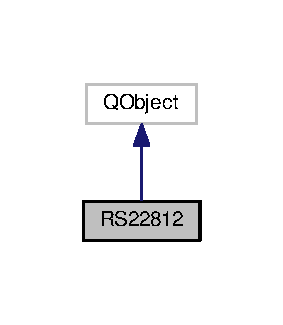
\includegraphics[width=136pt]{class_r_s22812__inherit__graph}
\end{center}
\end{figure}


Collaboration diagram for R\-S22812\-:\nopagebreak
\begin{figure}[H]
\begin{center}
\leavevmode
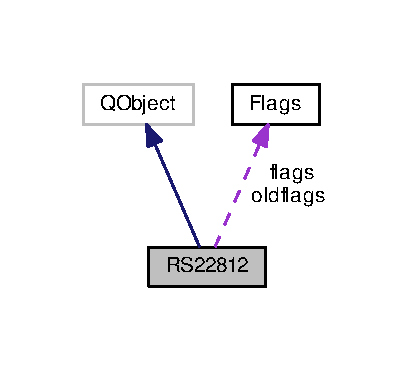
\includegraphics[width=198pt]{class_r_s22812__coll__graph}
\end{center}
\end{figure}
\subsection*{Public Slots}
\begin{DoxyCompactItemize}
\item 
void \hyperlink{class_r_s22812_a5de59c9521bc80e37745c8c3243d9229}{new\-Value} (const Q\-Byte\-Array \&data)
\begin{DoxyCompactList}\small\item\em Reads a new packet and reformats the data. \end{DoxyCompactList}\end{DoxyCompactItemize}
\subsection*{Signals}
\begin{DoxyCompactItemize}
\item 
void \hyperlink{class_r_s22812_a47691c122c8ad0716dc7c86b1bf01bb8}{new\-Mode} ()
\item 
void \hyperlink{class_r_s22812_afdbd28cc7f8abb95f13ad9d795c6c10d}{new\-Data} ()
\end{DoxyCompactItemize}
\subsection*{Public Member Functions}
\begin{DoxyCompactItemize}
\item 
\hyperlink{class_r_s22812_ac5e60fb0fe61e2be5db4d5caab46c827}{R\-S22812} (Q\-Object $\ast$parent=0)
\begin{DoxyCompactList}\small\item\em Constructor. \end{DoxyCompactList}\item 
float \hyperlink{class_r_s22812_a80e53a20cbe5c9c670e8b8309d043475}{get\-Val} () const 
\begin{DoxyCompactList}\small\item\em Returns the numeric value of the reading. \end{DoxyCompactList}\item 
\hyperlink{struct_flags}{Flags} \hyperlink{class_r_s22812_a4ae945cdd647a66f6e7d54f20f77502e}{get\-Flags} () const 
\begin{DoxyCompactList}\small\item\em Gets the current flags structure. \end{DoxyCompactList}\item 
Q\-String \hyperlink{class_r_s22812_aee09c692d82aacb68a598091ea4b6597}{get\-Digit\-String} () const 
\begin{DoxyCompactList}\small\item\em get\-Digit\-String It returns the multimeter reading in string format. \end{DoxyCompactList}\item 
uint \hyperlink{class_r_s22812_a72884c3f25b59129ac21dca9f68a664f}{get\-Mode} () const 
\begin{DoxyCompactList}\small\item\em get\-Mode \end{DoxyCompactList}\end{DoxyCompactItemize}
\subsection*{Private Member Functions}
\begin{DoxyCompactItemize}
\item 
bool \hyperlink{class_r_s22812_a551bff514434f8710316a06c529d1f3c}{mode\-Changed} ()
\begin{DoxyCompactList}\small\item\em Checks the flags structure to see whether the read mode changed. \end{DoxyCompactList}\item 
Q\-String \hyperlink{class_r_s22812_aee6ba6536ad3d47239501d812d5db994}{byte2\-Digit} (uchar byte)
\begin{DoxyCompactList}\small\item\em Translates the R\-S 22-\/812 byte value of the \hyperlink{class_l_c_d}{L\-C\-D} mapping into a digit. \end{DoxyCompactList}\item 
void \hyperlink{class_r_s22812_a64f4658259e355d64dcaaa92eac65e93}{reset\-Flags} (\hyperlink{struct_flags}{Flags} \&f)
\begin{DoxyCompactList}\small\item\em Sets all the flags to false. \end{DoxyCompactList}\end{DoxyCompactItemize}
\subsection*{Private Attributes}
\begin{DoxyCompactItemize}
\item 
uint \hyperlink{class_r_s22812_a368cc94b2c66bdc6d456e413de9217be}{mode}
\item 
\hyperlink{struct_flags}{Flags} \hyperlink{class_r_s22812_a6c8e4c27f876fdfd10bf153b36bd6254}{flags}
\item 
\hyperlink{struct_flags}{Flags} \hyperlink{class_r_s22812_a167304591d2e351f70975b608718946b}{oldflags}
\item 
Q\-String \hyperlink{class_r_s22812_a4514e9e982441cab9143a9c36a64429c}{digits}
\end{DoxyCompactItemize}


\subsection{Detailed Description}
Decoding of the data sent by the Radio Shack 22-\/812. 

Part of the information was obtained from \href{http://sigrok.org/wiki/RadioShack_22-812}{\tt http\-://sigrok.\-org/wiki/\-Radio\-Shack\-\_\-22-\/812} and \href{https://code.google.com/archive/p/rs22812/}{\tt https\-://code.\-google.\-com/archive/p/rs22812/}

R\-S 22-\/812 sends 9-\/bytes packets. Each packect is a mapping of the \hyperlink{class_l_c_d}{L\-C\-D} of the screen plus some extra information. \begin{DoxyVerb}                                    Bit
    Byte    7       6       5       4       3       2       1       0
    0       ---------------------- Mode -----------------------------
    1       Hz      Ohms    K       M       F       A       V       m
    2       u       n       dBm     s       %       hFE     REL     MIN
    3       4D      4C      4G      4B      DP3     4E      4F      4A
    4       3D      3C      3G      3B      DP2     3E      3F      3A
    5       2D      2C      2G      2B      DP1     2E      2F      2A
    6       1D      1C      1G      1B      MAX     1E      1F      1A
    7       Beep    Diode   Bat     Hold    -       ~       RS232   Auto
    8       -------------------- Checksum ---------------------------
\end{DoxyVerb}
 The L\-E\-D mapping is\-: \begin{DoxyVerb}    |--A--|
    |     |
    F     B
    |     |
    |--G--|
    |     |
    E     C
    |     |
    |--D--|
\end{DoxyVerb}
 So, the equivalence between int value and digit are\-:

215 \-: \char`\"{}0\char`\"{}, 80 \-: \char`\"{}1\char`\"{}, 181 \-: \char`\"{}2\char`\"{}, 241 \-: \char`\"{}3\char`\"{}, 114 \-: \char`\"{}4\char`\"{},\par
 227 \-: \char`\"{}5\char`\"{}, 231 \-: \char`\"{}6\char`\"{}, 81 \-: \char`\"{}7\char`\"{}, 247 \-: \char`\"{}8\char`\"{}, 243 \-: \char`\"{}9\char`\"{}, 39 \-: \char`\"{}\-F\char`\"{},\par
 55 \-: \char`\"{}\-P\char`\"{}, 167 \-: \char`\"{}\-E\char`\"{}, 135 \-: \char`\"{}\-C\char`\"{}, 134 \-: \char`\"{}\-L\char`\"{}, 118 \-: \char`\"{}\-H\char`\"{}, 6 \-: \char`\"{}\-I\char`\"{},\par
 102 \-: \char`\"{}h\char`\"{}, 36 \-: \char`\"{}r\char`\"{}, 166 \-: \char`\"{}t\char`\"{}, 100 \-: \char`\"{}n\char`\"{}, 32 \-: \char`\"{}-\/\char`\"{}, 0 \-: \char`\"{} \char`\"{}\par
 And the possible modes are\-:

\begin{TabularC}{3}
\hline
\rowcolor{lightgray}{\bf . }&{\bf . }&{\bf .  }\\\cline{1-3}
0=D\-C V &1=A\-C V &2=D\-C u\-A \\\cline{1-3}
3=D\-C m\-A &4=D\-C A &5=A\-C u\-A \\\cline{1-3}
6=A\-C m\-A &7=A\-C A &8=O\-H\-M \\\cline{1-3}
9=C\-A\-P &10=H\-Z &11=N\-E\-T H\-Z \\\cline{1-3}
12=A\-M\-P H\-Z &13=D\-U\-T\-Y &14=N\-E\-T D\-U\-T\-Y \\\cline{1-3}
15=A\-M\-P D\-U\-T\-Y &16=W\-I\-D\-T\-H &17=N\-E\-T W\-I\-D\-T\-H \\\cline{1-3}
18=A\-M\-P W\-I\-D\-T\-H &19=D\-I\-O\-D\-E &20=C\-O\-N\-T \\\cline{1-3}
21=H\-F\-E &22=L\-O\-G\-I\-C &23=D\-B\-M \\\cline{1-3}
24=E\-F &25=T\-E\-M\-P &. \\\cline{1-3}
\end{TabularC}


\subsection{Constructor \& Destructor Documentation}
\hypertarget{class_r_s22812_ac5e60fb0fe61e2be5db4d5caab46c827}{\index{R\-S22812@{R\-S22812}!R\-S22812@{R\-S22812}}
\index{R\-S22812@{R\-S22812}!RS22812@{R\-S22812}}
\subsubsection[{R\-S22812}]{\setlength{\rightskip}{0pt plus 5cm}R\-S22812\-::\-R\-S22812 (
\begin{DoxyParamCaption}
\item[{Q\-Object $\ast$}]{parent = {\ttfamily 0}}
\end{DoxyParamCaption}
)\hspace{0.3cm}{\ttfamily [explicit]}}}\label{class_r_s22812_ac5e60fb0fe61e2be5db4d5caab46c827}


Constructor. 


\begin{DoxyParams}{Parameters}
{\em parent} & It sets the mode to 0 and resets all the flags. \\
\hline
\end{DoxyParams}


Here is the call graph for this function\-:
\nopagebreak
\begin{figure}[H]
\begin{center}
\leavevmode
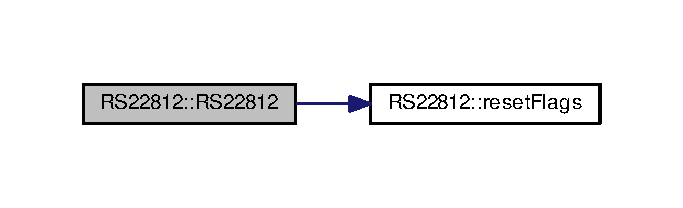
\includegraphics[width=328pt]{class_r_s22812_ac5e60fb0fe61e2be5db4d5caab46c827_cgraph}
\end{center}
\end{figure}




\subsection{Member Function Documentation}
\hypertarget{class_r_s22812_aee6ba6536ad3d47239501d812d5db994}{\index{R\-S22812@{R\-S22812}!byte2\-Digit@{byte2\-Digit}}
\index{byte2\-Digit@{byte2\-Digit}!RS22812@{R\-S22812}}
\subsubsection[{byte2\-Digit}]{\setlength{\rightskip}{0pt plus 5cm}Q\-String R\-S22812\-::byte2\-Digit (
\begin{DoxyParamCaption}
\item[{uchar}]{byte}
\end{DoxyParamCaption}
)\hspace{0.3cm}{\ttfamily [private]}}}\label{class_r_s22812_aee6ba6536ad3d47239501d812d5db994}


Translates the R\-S 22-\/812 byte value of the \hyperlink{class_l_c_d}{L\-C\-D} mapping into a digit. 


\begin{DoxyParams}{Parameters}
{\em byte} & R\-S 22-\/812 byte value \\
\hline
\end{DoxyParams}
\begin{DoxyReturn}{Returns}
String with the equivalent digit. 
\end{DoxyReturn}


Here is the caller graph for this function\-:
\nopagebreak
\begin{figure}[H]
\begin{center}
\leavevmode
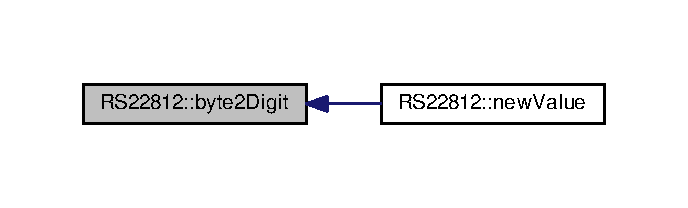
\includegraphics[width=330pt]{class_r_s22812_aee6ba6536ad3d47239501d812d5db994_icgraph}
\end{center}
\end{figure}


\hypertarget{class_r_s22812_aee09c692d82aacb68a598091ea4b6597}{\index{R\-S22812@{R\-S22812}!get\-Digit\-String@{get\-Digit\-String}}
\index{get\-Digit\-String@{get\-Digit\-String}!RS22812@{R\-S22812}}
\subsubsection[{get\-Digit\-String}]{\setlength{\rightskip}{0pt plus 5cm}Q\-String R\-S22812\-::get\-Digit\-String (
\begin{DoxyParamCaption}
{}
\end{DoxyParamCaption}
) const\hspace{0.3cm}{\ttfamily [inline]}}}\label{class_r_s22812_aee09c692d82aacb68a598091ea4b6597}


get\-Digit\-String It returns the multimeter reading in string format. 

\begin{DoxyReturn}{Returns}

\end{DoxyReturn}


Here is the caller graph for this function\-:
\nopagebreak
\begin{figure}[H]
\begin{center}
\leavevmode
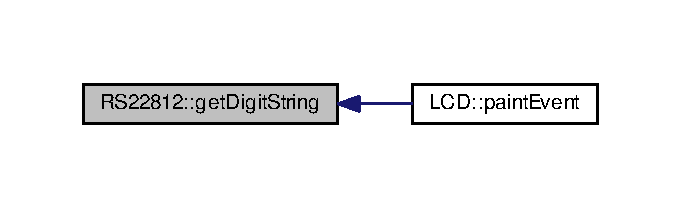
\includegraphics[width=327pt]{class_r_s22812_aee09c692d82aacb68a598091ea4b6597_icgraph}
\end{center}
\end{figure}


\hypertarget{class_r_s22812_a4ae945cdd647a66f6e7d54f20f77502e}{\index{R\-S22812@{R\-S22812}!get\-Flags@{get\-Flags}}
\index{get\-Flags@{get\-Flags}!RS22812@{R\-S22812}}
\subsubsection[{get\-Flags}]{\setlength{\rightskip}{0pt plus 5cm}{\bf Flags} R\-S22812\-::get\-Flags (
\begin{DoxyParamCaption}
{}
\end{DoxyParamCaption}
) const\hspace{0.3cm}{\ttfamily [inline]}}}\label{class_r_s22812_a4ae945cdd647a66f6e7d54f20f77502e}


Gets the current flags structure. 

\begin{DoxyReturn}{Returns}

\end{DoxyReturn}


Here is the caller graph for this function\-:
\nopagebreak
\begin{figure}[H]
\begin{center}
\leavevmode
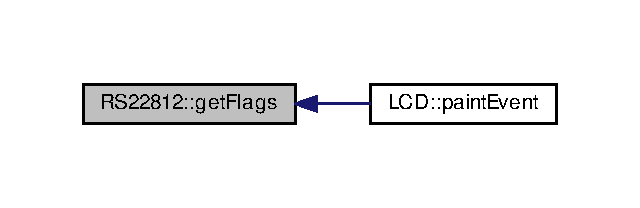
\includegraphics[width=307pt]{class_r_s22812_a4ae945cdd647a66f6e7d54f20f77502e_icgraph}
\end{center}
\end{figure}


\hypertarget{class_r_s22812_a72884c3f25b59129ac21dca9f68a664f}{\index{R\-S22812@{R\-S22812}!get\-Mode@{get\-Mode}}
\index{get\-Mode@{get\-Mode}!RS22812@{R\-S22812}}
\subsubsection[{get\-Mode}]{\setlength{\rightskip}{0pt plus 5cm}uint R\-S22812\-::get\-Mode (
\begin{DoxyParamCaption}
{}
\end{DoxyParamCaption}
) const\hspace{0.3cm}{\ttfamily [inline]}}}\label{class_r_s22812_a72884c3f25b59129ac21dca9f68a664f}


get\-Mode 

\begin{DoxyReturn}{Returns}
It returns the mode on which the multimeter is working. 
\end{DoxyReturn}


Here is the caller graph for this function\-:
\nopagebreak
\begin{figure}[H]
\begin{center}
\leavevmode
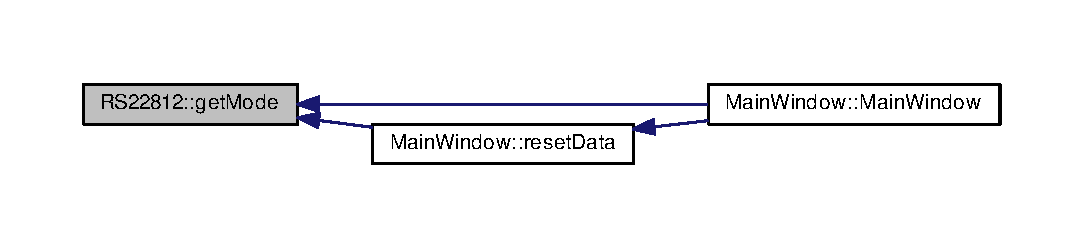
\includegraphics[width=350pt]{class_r_s22812_a72884c3f25b59129ac21dca9f68a664f_icgraph}
\end{center}
\end{figure}


\hypertarget{class_r_s22812_a80e53a20cbe5c9c670e8b8309d043475}{\index{R\-S22812@{R\-S22812}!get\-Val@{get\-Val}}
\index{get\-Val@{get\-Val}!RS22812@{R\-S22812}}
\subsubsection[{get\-Val}]{\setlength{\rightskip}{0pt plus 5cm}float R\-S22812\-::get\-Val (
\begin{DoxyParamCaption}
{}
\end{DoxyParamCaption}
) const}}\label{class_r_s22812_a80e53a20cbe5c9c670e8b8309d043475}


Returns the numeric value of the reading. 

\begin{DoxyReturn}{Returns}

\end{DoxyReturn}


Here is the caller graph for this function\-:
\nopagebreak
\begin{figure}[H]
\begin{center}
\leavevmode
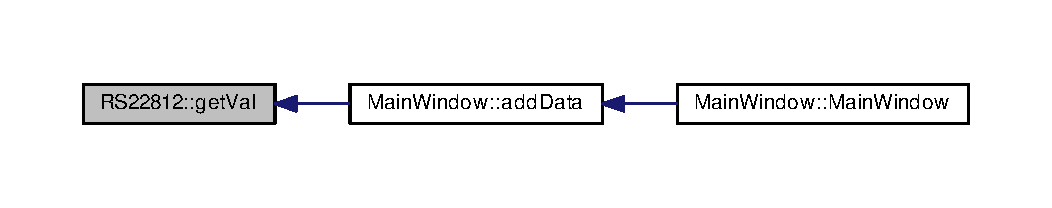
\includegraphics[width=350pt]{class_r_s22812_a80e53a20cbe5c9c670e8b8309d043475_icgraph}
\end{center}
\end{figure}


\hypertarget{class_r_s22812_a551bff514434f8710316a06c529d1f3c}{\index{R\-S22812@{R\-S22812}!mode\-Changed@{mode\-Changed}}
\index{mode\-Changed@{mode\-Changed}!RS22812@{R\-S22812}}
\subsubsection[{mode\-Changed}]{\setlength{\rightskip}{0pt plus 5cm}bool R\-S22812\-::mode\-Changed (
\begin{DoxyParamCaption}
{}
\end{DoxyParamCaption}
)\hspace{0.3cm}{\ttfamily [private]}}}\label{class_r_s22812_a551bff514434f8710316a06c529d1f3c}


Checks the flags structure to see whether the read mode changed. 

\begin{DoxyReturn}{Returns}

\end{DoxyReturn}


Here is the caller graph for this function\-:
\nopagebreak
\begin{figure}[H]
\begin{center}
\leavevmode
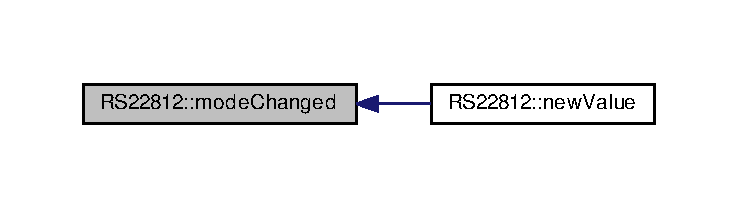
\includegraphics[width=350pt]{class_r_s22812_a551bff514434f8710316a06c529d1f3c_icgraph}
\end{center}
\end{figure}


\hypertarget{class_r_s22812_afdbd28cc7f8abb95f13ad9d795c6c10d}{\index{R\-S22812@{R\-S22812}!new\-Data@{new\-Data}}
\index{new\-Data@{new\-Data}!RS22812@{R\-S22812}}
\subsubsection[{new\-Data}]{\setlength{\rightskip}{0pt plus 5cm}void R\-S22812\-::new\-Data (
\begin{DoxyParamCaption}
{}
\end{DoxyParamCaption}
)\hspace{0.3cm}{\ttfamily [signal]}}}\label{class_r_s22812_afdbd28cc7f8abb95f13ad9d795c6c10d}


Here is the caller graph for this function\-:
\nopagebreak
\begin{figure}[H]
\begin{center}
\leavevmode
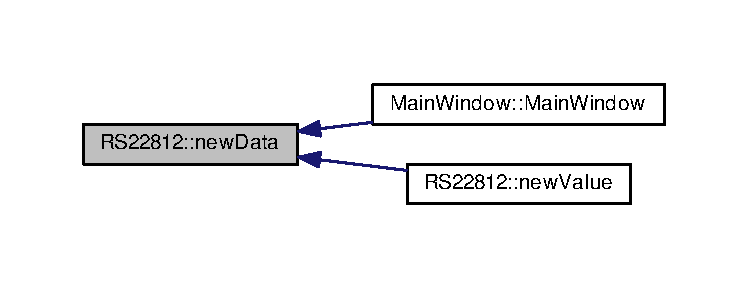
\includegraphics[width=350pt]{class_r_s22812_afdbd28cc7f8abb95f13ad9d795c6c10d_icgraph}
\end{center}
\end{figure}


\hypertarget{class_r_s22812_a47691c122c8ad0716dc7c86b1bf01bb8}{\index{R\-S22812@{R\-S22812}!new\-Mode@{new\-Mode}}
\index{new\-Mode@{new\-Mode}!RS22812@{R\-S22812}}
\subsubsection[{new\-Mode}]{\setlength{\rightskip}{0pt plus 5cm}void R\-S22812\-::new\-Mode (
\begin{DoxyParamCaption}
{}
\end{DoxyParamCaption}
)\hspace{0.3cm}{\ttfamily [signal]}}}\label{class_r_s22812_a47691c122c8ad0716dc7c86b1bf01bb8}


Here is the caller graph for this function\-:
\nopagebreak
\begin{figure}[H]
\begin{center}
\leavevmode
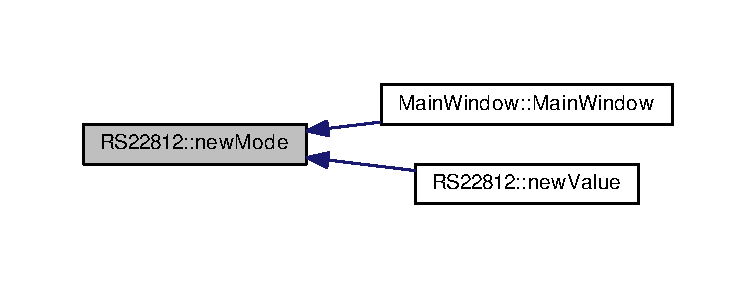
\includegraphics[width=350pt]{class_r_s22812_a47691c122c8ad0716dc7c86b1bf01bb8_icgraph}
\end{center}
\end{figure}


\hypertarget{class_r_s22812_a5de59c9521bc80e37745c8c3243d9229}{\index{R\-S22812@{R\-S22812}!new\-Value@{new\-Value}}
\index{new\-Value@{new\-Value}!RS22812@{R\-S22812}}
\subsubsection[{new\-Value}]{\setlength{\rightskip}{0pt plus 5cm}void R\-S22812\-::new\-Value (
\begin{DoxyParamCaption}
\item[{const Q\-Byte\-Array \&}]{data}
\end{DoxyParamCaption}
)\hspace{0.3cm}{\ttfamily [slot]}}}\label{class_r_s22812_a5de59c9521bc80e37745c8c3243d9229}


Reads a new packet and reformats the data. 


\begin{DoxyParams}{Parameters}
{\em data} & \\
\hline
\end{DoxyParams}


Here is the call graph for this function\-:
\nopagebreak
\begin{figure}[H]
\begin{center}
\leavevmode
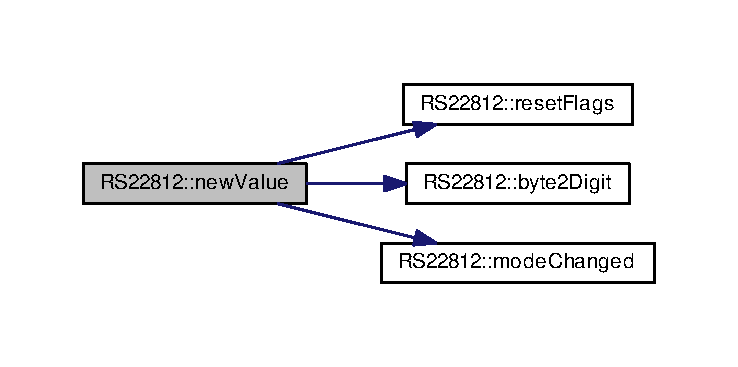
\includegraphics[width=350pt]{class_r_s22812_a5de59c9521bc80e37745c8c3243d9229_cgraph}
\end{center}
\end{figure}


\hypertarget{class_r_s22812_a64f4658259e355d64dcaaa92eac65e93}{\index{R\-S22812@{R\-S22812}!reset\-Flags@{reset\-Flags}}
\index{reset\-Flags@{reset\-Flags}!RS22812@{R\-S22812}}
\subsubsection[{reset\-Flags}]{\setlength{\rightskip}{0pt plus 5cm}void R\-S22812\-::reset\-Flags (
\begin{DoxyParamCaption}
\item[{{\bf Flags} \&}]{f}
\end{DoxyParamCaption}
)\hspace{0.3cm}{\ttfamily [private]}}}\label{class_r_s22812_a64f4658259e355d64dcaaa92eac65e93}


Sets all the flags to false. 



Here is the caller graph for this function\-:
\nopagebreak
\begin{figure}[H]
\begin{center}
\leavevmode
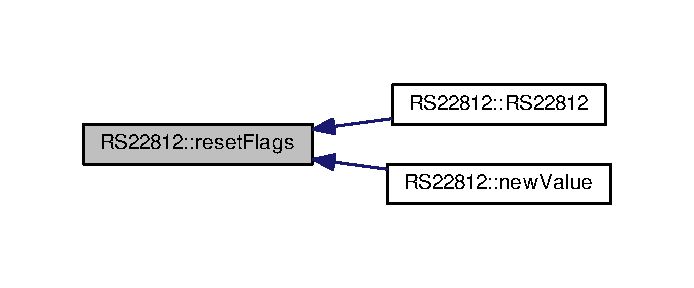
\includegraphics[width=333pt]{class_r_s22812_a64f4658259e355d64dcaaa92eac65e93_icgraph}
\end{center}
\end{figure}




\subsection{Member Data Documentation}
\hypertarget{class_r_s22812_a4514e9e982441cab9143a9c36a64429c}{\index{R\-S22812@{R\-S22812}!digits@{digits}}
\index{digits@{digits}!RS22812@{R\-S22812}}
\subsubsection[{digits}]{\setlength{\rightskip}{0pt plus 5cm}Q\-String R\-S22812\-::digits\hspace{0.3cm}{\ttfamily [private]}}}\label{class_r_s22812_a4514e9e982441cab9143a9c36a64429c}
\hypertarget{class_r_s22812_a6c8e4c27f876fdfd10bf153b36bd6254}{\index{R\-S22812@{R\-S22812}!flags@{flags}}
\index{flags@{flags}!RS22812@{R\-S22812}}
\subsubsection[{flags}]{\setlength{\rightskip}{0pt plus 5cm}{\bf Flags} R\-S22812\-::flags\hspace{0.3cm}{\ttfamily [private]}}}\label{class_r_s22812_a6c8e4c27f876fdfd10bf153b36bd6254}
\hypertarget{class_r_s22812_a368cc94b2c66bdc6d456e413de9217be}{\index{R\-S22812@{R\-S22812}!mode@{mode}}
\index{mode@{mode}!RS22812@{R\-S22812}}
\subsubsection[{mode}]{\setlength{\rightskip}{0pt plus 5cm}uint R\-S22812\-::mode\hspace{0.3cm}{\ttfamily [private]}}}\label{class_r_s22812_a368cc94b2c66bdc6d456e413de9217be}
\hypertarget{class_r_s22812_a167304591d2e351f70975b608718946b}{\index{R\-S22812@{R\-S22812}!oldflags@{oldflags}}
\index{oldflags@{oldflags}!RS22812@{R\-S22812}}
\subsubsection[{oldflags}]{\setlength{\rightskip}{0pt plus 5cm}{\bf Flags} R\-S22812\-::oldflags\hspace{0.3cm}{\ttfamily [private]}}}\label{class_r_s22812_a167304591d2e351f70975b608718946b}


The documentation for this class was generated from the following files\-:\begin{DoxyCompactItemize}
\item 
\hyperlink{rs22812_8h}{rs22812.\-h}\item 
build-\/multimeter\-G\-U\-I-\/\-Desktop-\/\-Debug/\hyperlink{moc__rs22812_8cpp}{moc\-\_\-rs22812.\-cpp}\item 
\hyperlink{rs22812_8cpp}{rs22812.\-cpp}\end{DoxyCompactItemize}

\hypertarget{class_serial_port}{\section{Serial\-Port Class Reference}
\label{class_serial_port}\index{Serial\-Port@{Serial\-Port}}
}


Class to manage the communication with a serial port.  




{\ttfamily \#include $<$serialport.\-h$>$}



Inheritance diagram for Serial\-Port\-:\nopagebreak
\begin{figure}[H]
\begin{center}
\leavevmode
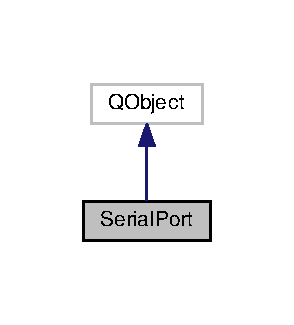
\includegraphics[width=141pt]{class_serial_port__inherit__graph}
\end{center}
\end{figure}


Collaboration diagram for Serial\-Port\-:\nopagebreak
\begin{figure}[H]
\begin{center}
\leavevmode
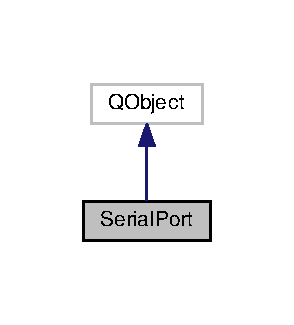
\includegraphics[width=141pt]{class_serial_port__coll__graph}
\end{center}
\end{figure}
\subsection*{Public Slots}
\begin{DoxyCompactItemize}
\item 
void \hyperlink{class_serial_port_a76a7bb63e3f581ccb55a5951bf97a4e3}{ready} ()
\begin{DoxyCompactList}\small\item\em \hyperlink{class_serial_port_a76a7bb63e3f581ccb55a5951bf97a4e3}{Serial\-Port\-::ready} Re-\/emits the ready\-Read signal. \end{DoxyCompactList}\end{DoxyCompactItemize}
\subsection*{Signals}
\begin{DoxyCompactItemize}
\item 
void \hyperlink{class_serial_port_a3ec0fe7fd001c56fb95e010da11817c0}{ready\-Read} (Q\-Byte\-Array \hyperlink{class_serial_port_af5ff5c504f070840bd28ee371f353f05}{buffer})
\end{DoxyCompactItemize}
\subsection*{Public Member Functions}
\begin{DoxyCompactItemize}
\item 
\hyperlink{class_serial_port_ae68e4a28e607b4acbab2c2a894cb3e2b}{Serial\-Port} (Q\-Object $\ast$parent=0)
\begin{DoxyCompactList}\small\item\em \hyperlink{class_serial_port_ae68e4a28e607b4acbab2c2a894cb3e2b}{Serial\-Port\-::\-Serial\-Port} Constructor. \end{DoxyCompactList}\item 
\hyperlink{class_serial_port_a8e09f366ed9b26b0456b66ae7bd8c702}{$\sim$\-Serial\-Port} ()
\begin{DoxyCompactList}\small\item\em \hyperlink{class_serial_port_a8e09f366ed9b26b0456b66ae7bd8c702}{Serial\-Port\-::$\sim$\-Serial\-Port}. \end{DoxyCompactList}\item 
bool \hyperlink{class_serial_port_a746e1ff02d45d8bf6b94e8bcbde6bb0d}{open\-Port} (const Q\-String port\-Name)
\begin{DoxyCompactList}\small\item\em \hyperlink{class_serial_port_a746e1ff02d45d8bf6b94e8bcbde6bb0d}{Serial\-Port\-::open\-Port} Opens a serial port for reading. If port name is empty, it does nothing. If port name is not available. Does nothing and raises a warning. \end{DoxyCompactList}\item 
bool \hyperlink{class_serial_port_a71c52f501f57ab491d0dc83cbc5e6a14}{close\-Port} ()
\begin{DoxyCompactList}\small\item\em \hyperlink{class_serial_port_a71c52f501f57ab491d0dc83cbc5e6a14}{Serial\-Port\-::close\-Port}. \end{DoxyCompactList}\item 
Q\-List$<$ Q\-Serial\-Port\-Info $>$ \hyperlink{class_serial_port_acd94c96dd2608f90a9ead0ced2742d17}{list\-Ports} ()
\begin{DoxyCompactList}\small\item\em \hyperlink{class_serial_port_acd94c96dd2608f90a9ead0ced2742d17}{Serial\-Port\-::list\-Ports} Obtains and return the list of available ports. \end{DoxyCompactList}\end{DoxyCompactItemize}
\subsection*{Private Member Functions}
\begin{DoxyCompactItemize}
\item 
void \hyperlink{class_serial_port_a708a04f46660c9803112fda4f60defe1}{read\-Port} ()
\begin{DoxyCompactList}\small\item\em \hyperlink{class_serial_port_a708a04f46660c9803112fda4f60defe1}{Serial\-Port\-::read\-Port} Reads the available data. \end{DoxyCompactList}\end{DoxyCompactItemize}
\subsection*{Private Attributes}
\begin{DoxyCompactItemize}
\item 
Q\-Serial\-Port\-Info $\ast$ \hyperlink{class_serial_port_aead0028dd7ba1073c5a0cf6f1775106b}{ports}
\item 
Q\-Serial\-Port $\ast$ \hyperlink{class_serial_port_abf454cb55d0053b354080a0dd6a43800}{active\-Port}
\item 
bool \hyperlink{class_serial_port_ab4a0ae7dd5d94991088247289935424d}{is\-Open}
\item 
Q\-Byte\-Array \hyperlink{class_serial_port_af5ff5c504f070840bd28ee371f353f05}{buffer}
\item 
Q\-Meta\-Object\-::\-Connection \hyperlink{class_serial_port_a63896cd014af7968402b8e7f051f24b3}{read\-Connect}
\item 
const Q\-Serial\-Port\-::\-Open\-Mode \hyperlink{class_serial_port_a92c94e506ac3ae86ea1e787c0d7b138f}{M\-O\-D\-E} =Q\-Serial\-Port\-::\-Read\-Only
\end{DoxyCompactItemize}
\subsection*{Static Private Attributes}
\begin{DoxyCompactItemize}
\item 
static const Q\-Serial\-Port\-::\-Baud\-Rate \hyperlink{class_serial_port_af5e3812b185f5f72c3ac1c298497694b}{B\-A\-U\-D\-R\-A\-T\-E} =Q\-Serial\-Port\-::\-Baud4800
\item 
static const Q\-Serial\-Port\-::\-Data\-Bits \hyperlink{class_serial_port_a74455f210ee1c4704daf3347b7d2b088}{D\-A\-T\-A\-B\-I\-T\-S} =Q\-Serial\-Port\-::\-Data8
\item 
static const Q\-Serial\-Port\-::\-Stop\-Bits \hyperlink{class_serial_port_a52f45df73cda27a0c096ddbfa53ff025}{S\-T\-O\-P\-B\-I\-T\-S} =Q\-Serial\-Port\-::\-One\-Stop
\item 
static const Q\-Serial\-Port\-::\-Parity \hyperlink{class_serial_port_afb8f52adfc0898451eb78eb5961b125c}{P\-A\-R\-I\-T\-Y} =Q\-Serial\-Port\-::\-No\-Parity
\end{DoxyCompactItemize}


\subsection{Detailed Description}
Class to manage the communication with a serial port. 

R\-S 22-\/812 sends 9bytes long packets with the codified information. This class is meant to read those packets and send it to the \hyperlink{class_r_s22812}{R\-S22812} class to store and interpret. 

\subsection{Constructor \& Destructor Documentation}
\hypertarget{class_serial_port_ae68e4a28e607b4acbab2c2a894cb3e2b}{\index{Serial\-Port@{Serial\-Port}!Serial\-Port@{Serial\-Port}}
\index{Serial\-Port@{Serial\-Port}!SerialPort@{Serial\-Port}}
\subsubsection[{Serial\-Port}]{\setlength{\rightskip}{0pt plus 5cm}Serial\-Port\-::\-Serial\-Port (
\begin{DoxyParamCaption}
\item[{Q\-Object $\ast$}]{parent = {\ttfamily 0}}
\end{DoxyParamCaption}
)\hspace{0.3cm}{\ttfamily [explicit]}}}\label{class_serial_port_ae68e4a28e607b4acbab2c2a894cb3e2b}


\hyperlink{class_serial_port_ae68e4a28e607b4acbab2c2a894cb3e2b}{Serial\-Port\-::\-Serial\-Port} Constructor. 


\begin{DoxyParams}{Parameters}
{\em parent} & \\
\hline
\end{DoxyParams}
\hypertarget{class_serial_port_a8e09f366ed9b26b0456b66ae7bd8c702}{\index{Serial\-Port@{Serial\-Port}!$\sim$\-Serial\-Port@{$\sim$\-Serial\-Port}}
\index{$\sim$\-Serial\-Port@{$\sim$\-Serial\-Port}!SerialPort@{Serial\-Port}}
\subsubsection[{$\sim$\-Serial\-Port}]{\setlength{\rightskip}{0pt plus 5cm}Serial\-Port\-::$\sim$\-Serial\-Port (
\begin{DoxyParamCaption}
{}
\end{DoxyParamCaption}
)}}\label{class_serial_port_a8e09f366ed9b26b0456b66ae7bd8c702}


\hyperlink{class_serial_port_a8e09f366ed9b26b0456b66ae7bd8c702}{Serial\-Port\-::$\sim$\-Serial\-Port}. 



Here is the call graph for this function\-:\nopagebreak
\begin{figure}[H]
\begin{center}
\leavevmode
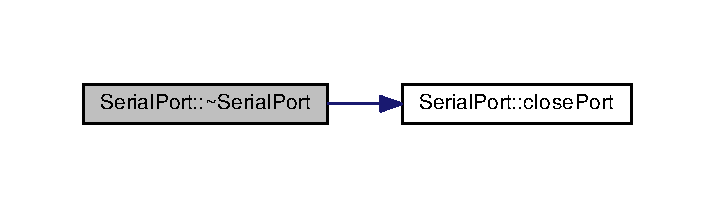
\includegraphics[width=343pt]{class_serial_port_a8e09f366ed9b26b0456b66ae7bd8c702_cgraph}
\end{center}
\end{figure}




\subsection{Member Function Documentation}
\hypertarget{class_serial_port_a71c52f501f57ab491d0dc83cbc5e6a14}{\index{Serial\-Port@{Serial\-Port}!close\-Port@{close\-Port}}
\index{close\-Port@{close\-Port}!SerialPort@{Serial\-Port}}
\subsubsection[{close\-Port}]{\setlength{\rightskip}{0pt plus 5cm}bool Serial\-Port\-::close\-Port (
\begin{DoxyParamCaption}
{}
\end{DoxyParamCaption}
)}}\label{class_serial_port_a71c52f501f57ab491d0dc83cbc5e6a14}


\hyperlink{class_serial_port_a71c52f501f57ab491d0dc83cbc5e6a14}{Serial\-Port\-::close\-Port}. 

\begin{DoxyReturn}{Returns}

\end{DoxyReturn}


Here is the caller graph for this function\-:\nopagebreak
\begin{figure}[H]
\begin{center}
\leavevmode
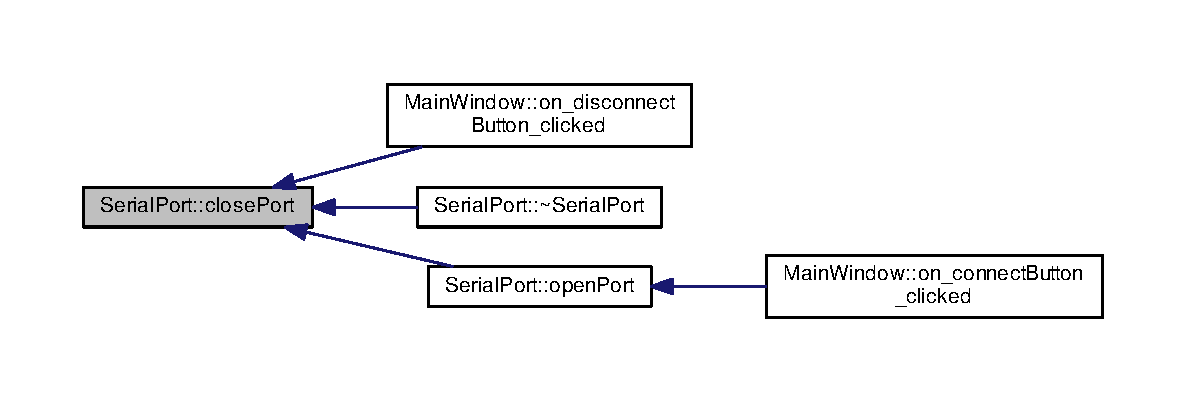
\includegraphics[width=350pt]{class_serial_port_a71c52f501f57ab491d0dc83cbc5e6a14_icgraph}
\end{center}
\end{figure}


\hypertarget{class_serial_port_acd94c96dd2608f90a9ead0ced2742d17}{\index{Serial\-Port@{Serial\-Port}!list\-Ports@{list\-Ports}}
\index{list\-Ports@{list\-Ports}!SerialPort@{Serial\-Port}}
\subsubsection[{list\-Ports}]{\setlength{\rightskip}{0pt plus 5cm}Q\-List$<$ Q\-Serial\-Port\-Info $>$ Serial\-Port\-::list\-Ports (
\begin{DoxyParamCaption}
{}
\end{DoxyParamCaption}
)}}\label{class_serial_port_acd94c96dd2608f90a9ead0ced2742d17}


\hyperlink{class_serial_port_acd94c96dd2608f90a9ead0ced2742d17}{Serial\-Port\-::list\-Ports} Obtains and return the list of available ports. 

\begin{DoxyReturn}{Returns}
Q\-List$<$\-Q\-Serial\-Port\-Info$>$ 
\end{DoxyReturn}


Here is the caller graph for this function\-:\nopagebreak
\begin{figure}[H]
\begin{center}
\leavevmode
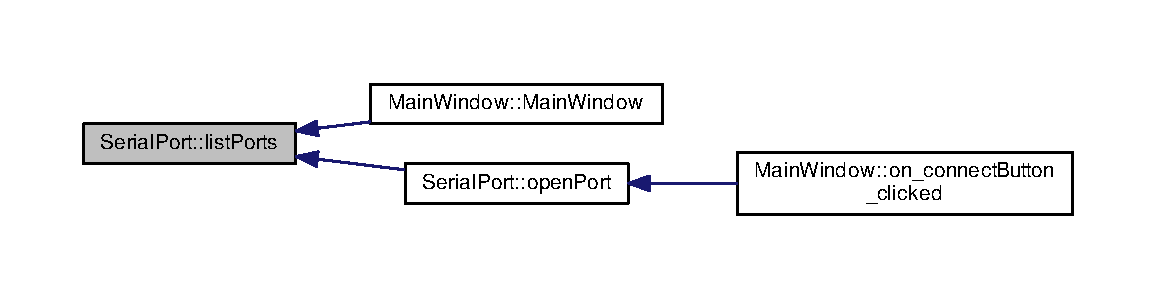
\includegraphics[width=350pt]{class_serial_port_acd94c96dd2608f90a9ead0ced2742d17_icgraph}
\end{center}
\end{figure}


\hypertarget{class_serial_port_a746e1ff02d45d8bf6b94e8bcbde6bb0d}{\index{Serial\-Port@{Serial\-Port}!open\-Port@{open\-Port}}
\index{open\-Port@{open\-Port}!SerialPort@{Serial\-Port}}
\subsubsection[{open\-Port}]{\setlength{\rightskip}{0pt plus 5cm}bool Serial\-Port\-::open\-Port (
\begin{DoxyParamCaption}
\item[{const Q\-String}]{port\-Name}
\end{DoxyParamCaption}
)}}\label{class_serial_port_a746e1ff02d45d8bf6b94e8bcbde6bb0d}


\hyperlink{class_serial_port_a746e1ff02d45d8bf6b94e8bcbde6bb0d}{Serial\-Port\-::open\-Port} Opens a serial port for reading. If port name is empty, it does nothing. If port name is not available. Does nothing and raises a warning. 


\begin{DoxyParams}{Parameters}
{\em port\-Name} & Name of the port as returned from Q\-Serial\-Port\-Info. \\
\hline
\end{DoxyParams}
\begin{DoxyReturn}{Returns}
If sucessful, returns 1. Else it returns 0; 
\end{DoxyReturn}


Here is the call graph for this function\-:\nopagebreak
\begin{figure}[H]
\begin{center}
\leavevmode
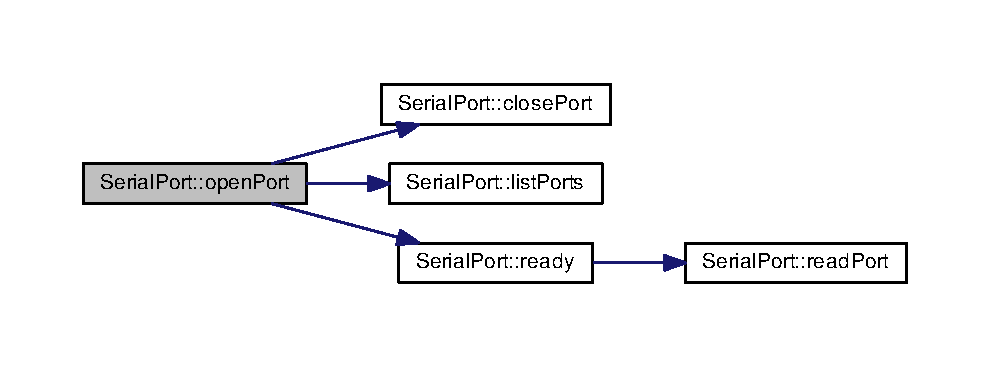
\includegraphics[width=350pt]{class_serial_port_a746e1ff02d45d8bf6b94e8bcbde6bb0d_cgraph}
\end{center}
\end{figure}




Here is the caller graph for this function\-:\nopagebreak
\begin{figure}[H]
\begin{center}
\leavevmode
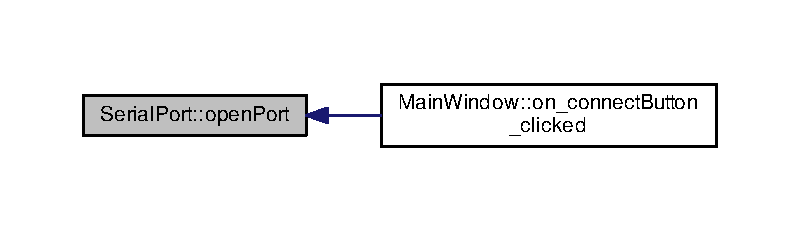
\includegraphics[width=350pt]{class_serial_port_a746e1ff02d45d8bf6b94e8bcbde6bb0d_icgraph}
\end{center}
\end{figure}


\hypertarget{class_serial_port_a708a04f46660c9803112fda4f60defe1}{\index{Serial\-Port@{Serial\-Port}!read\-Port@{read\-Port}}
\index{read\-Port@{read\-Port}!SerialPort@{Serial\-Port}}
\subsubsection[{read\-Port}]{\setlength{\rightskip}{0pt plus 5cm}void Serial\-Port\-::read\-Port (
\begin{DoxyParamCaption}
{}
\end{DoxyParamCaption}
)\hspace{0.3cm}{\ttfamily [private]}}}\label{class_serial_port_a708a04f46660c9803112fda4f60defe1}


\hyperlink{class_serial_port_a708a04f46660c9803112fda4f60defe1}{Serial\-Port\-::read\-Port} Reads the available data. 



Here is the caller graph for this function\-:\nopagebreak
\begin{figure}[H]
\begin{center}
\leavevmode
\includegraphics[width=350pt]{class_serial_port_a708a04f46660c9803112fda4f60defe1_icgraph}
\end{center}
\end{figure}


\hypertarget{class_serial_port_a76a7bb63e3f581ccb55a5951bf97a4e3}{\index{Serial\-Port@{Serial\-Port}!ready@{ready}}
\index{ready@{ready}!SerialPort@{Serial\-Port}}
\subsubsection[{ready}]{\setlength{\rightskip}{0pt plus 5cm}void Serial\-Port\-::ready (
\begin{DoxyParamCaption}
{}
\end{DoxyParamCaption}
)\hspace{0.3cm}{\ttfamily [slot]}}}\label{class_serial_port_a76a7bb63e3f581ccb55a5951bf97a4e3}


\hyperlink{class_serial_port_a76a7bb63e3f581ccb55a5951bf97a4e3}{Serial\-Port\-::ready} Re-\/emits the ready\-Read signal. 



Here is the call graph for this function\-:\nopagebreak
\begin{figure}[H]
\begin{center}
\leavevmode
\includegraphics[width=315pt]{class_serial_port_a76a7bb63e3f581ccb55a5951bf97a4e3_cgraph}
\end{center}
\end{figure}




Here is the caller graph for this function\-:\nopagebreak
\begin{figure}[H]
\begin{center}
\leavevmode
\includegraphics[width=350pt]{class_serial_port_a76a7bb63e3f581ccb55a5951bf97a4e3_icgraph}
\end{center}
\end{figure}


\hypertarget{class_serial_port_a3ec0fe7fd001c56fb95e010da11817c0}{\index{Serial\-Port@{Serial\-Port}!ready\-Read@{ready\-Read}}
\index{ready\-Read@{ready\-Read}!SerialPort@{Serial\-Port}}
\subsubsection[{ready\-Read}]{\setlength{\rightskip}{0pt plus 5cm}void Serial\-Port\-::ready\-Read (
\begin{DoxyParamCaption}
\item[{Q\-Byte\-Array}]{buffer}
\end{DoxyParamCaption}
)\hspace{0.3cm}{\ttfamily [signal]}}}\label{class_serial_port_a3ec0fe7fd001c56fb95e010da11817c0}


Here is the caller graph for this function\-:\nopagebreak
\begin{figure}[H]
\begin{center}
\leavevmode
\includegraphics[width=350pt]{class_serial_port_a3ec0fe7fd001c56fb95e010da11817c0_icgraph}
\end{center}
\end{figure}




\subsection{Member Data Documentation}
\hypertarget{class_serial_port_abf454cb55d0053b354080a0dd6a43800}{\index{Serial\-Port@{Serial\-Port}!active\-Port@{active\-Port}}
\index{active\-Port@{active\-Port}!SerialPort@{Serial\-Port}}
\subsubsection[{active\-Port}]{\setlength{\rightskip}{0pt plus 5cm}Q\-Serial\-Port$\ast$ Serial\-Port\-::active\-Port\hspace{0.3cm}{\ttfamily [private]}}}\label{class_serial_port_abf454cb55d0053b354080a0dd6a43800}
\hypertarget{class_serial_port_af5e3812b185f5f72c3ac1c298497694b}{\index{Serial\-Port@{Serial\-Port}!B\-A\-U\-D\-R\-A\-T\-E@{B\-A\-U\-D\-R\-A\-T\-E}}
\index{B\-A\-U\-D\-R\-A\-T\-E@{B\-A\-U\-D\-R\-A\-T\-E}!SerialPort@{Serial\-Port}}
\subsubsection[{B\-A\-U\-D\-R\-A\-T\-E}]{\setlength{\rightskip}{0pt plus 5cm}const Q\-Serial\-Port\-::\-Baud\-Rate Serial\-Port\-::\-B\-A\-U\-D\-R\-A\-T\-E =Q\-Serial\-Port\-::\-Baud4800\hspace{0.3cm}{\ttfamily [static]}, {\ttfamily [private]}}}\label{class_serial_port_af5e3812b185f5f72c3ac1c298497694b}
\hypertarget{class_serial_port_af5ff5c504f070840bd28ee371f353f05}{\index{Serial\-Port@{Serial\-Port}!buffer@{buffer}}
\index{buffer@{buffer}!SerialPort@{Serial\-Port}}
\subsubsection[{buffer}]{\setlength{\rightskip}{0pt plus 5cm}Q\-Byte\-Array Serial\-Port\-::buffer\hspace{0.3cm}{\ttfamily [private]}}}\label{class_serial_port_af5ff5c504f070840bd28ee371f353f05}
\hypertarget{class_serial_port_a74455f210ee1c4704daf3347b7d2b088}{\index{Serial\-Port@{Serial\-Port}!D\-A\-T\-A\-B\-I\-T\-S@{D\-A\-T\-A\-B\-I\-T\-S}}
\index{D\-A\-T\-A\-B\-I\-T\-S@{D\-A\-T\-A\-B\-I\-T\-S}!SerialPort@{Serial\-Port}}
\subsubsection[{D\-A\-T\-A\-B\-I\-T\-S}]{\setlength{\rightskip}{0pt plus 5cm}const Q\-Serial\-Port\-::\-Data\-Bits Serial\-Port\-::\-D\-A\-T\-A\-B\-I\-T\-S =Q\-Serial\-Port\-::\-Data8\hspace{0.3cm}{\ttfamily [static]}, {\ttfamily [private]}}}\label{class_serial_port_a74455f210ee1c4704daf3347b7d2b088}
\hypertarget{class_serial_port_ab4a0ae7dd5d94991088247289935424d}{\index{Serial\-Port@{Serial\-Port}!is\-Open@{is\-Open}}
\index{is\-Open@{is\-Open}!SerialPort@{Serial\-Port}}
\subsubsection[{is\-Open}]{\setlength{\rightskip}{0pt plus 5cm}bool Serial\-Port\-::is\-Open\hspace{0.3cm}{\ttfamily [private]}}}\label{class_serial_port_ab4a0ae7dd5d94991088247289935424d}
\hypertarget{class_serial_port_a92c94e506ac3ae86ea1e787c0d7b138f}{\index{Serial\-Port@{Serial\-Port}!M\-O\-D\-E@{M\-O\-D\-E}}
\index{M\-O\-D\-E@{M\-O\-D\-E}!SerialPort@{Serial\-Port}}
\subsubsection[{M\-O\-D\-E}]{\setlength{\rightskip}{0pt plus 5cm}const Q\-Serial\-Port\-::\-Open\-Mode Serial\-Port\-::\-M\-O\-D\-E =Q\-Serial\-Port\-::\-Read\-Only\hspace{0.3cm}{\ttfamily [private]}}}\label{class_serial_port_a92c94e506ac3ae86ea1e787c0d7b138f}
\hypertarget{class_serial_port_afb8f52adfc0898451eb78eb5961b125c}{\index{Serial\-Port@{Serial\-Port}!P\-A\-R\-I\-T\-Y@{P\-A\-R\-I\-T\-Y}}
\index{P\-A\-R\-I\-T\-Y@{P\-A\-R\-I\-T\-Y}!SerialPort@{Serial\-Port}}
\subsubsection[{P\-A\-R\-I\-T\-Y}]{\setlength{\rightskip}{0pt plus 5cm}const Q\-Serial\-Port\-::\-Parity Serial\-Port\-::\-P\-A\-R\-I\-T\-Y =Q\-Serial\-Port\-::\-No\-Parity\hspace{0.3cm}{\ttfamily [static]}, {\ttfamily [private]}}}\label{class_serial_port_afb8f52adfc0898451eb78eb5961b125c}
\hypertarget{class_serial_port_aead0028dd7ba1073c5a0cf6f1775106b}{\index{Serial\-Port@{Serial\-Port}!ports@{ports}}
\index{ports@{ports}!SerialPort@{Serial\-Port}}
\subsubsection[{ports}]{\setlength{\rightskip}{0pt plus 5cm}Q\-Serial\-Port\-Info$\ast$ Serial\-Port\-::ports\hspace{0.3cm}{\ttfamily [private]}}}\label{class_serial_port_aead0028dd7ba1073c5a0cf6f1775106b}
\hypertarget{class_serial_port_a63896cd014af7968402b8e7f051f24b3}{\index{Serial\-Port@{Serial\-Port}!read\-Connect@{read\-Connect}}
\index{read\-Connect@{read\-Connect}!SerialPort@{Serial\-Port}}
\subsubsection[{read\-Connect}]{\setlength{\rightskip}{0pt plus 5cm}Q\-Meta\-Object\-::\-Connection Serial\-Port\-::read\-Connect\hspace{0.3cm}{\ttfamily [private]}}}\label{class_serial_port_a63896cd014af7968402b8e7f051f24b3}
\hypertarget{class_serial_port_a52f45df73cda27a0c096ddbfa53ff025}{\index{Serial\-Port@{Serial\-Port}!S\-T\-O\-P\-B\-I\-T\-S@{S\-T\-O\-P\-B\-I\-T\-S}}
\index{S\-T\-O\-P\-B\-I\-T\-S@{S\-T\-O\-P\-B\-I\-T\-S}!SerialPort@{Serial\-Port}}
\subsubsection[{S\-T\-O\-P\-B\-I\-T\-S}]{\setlength{\rightskip}{0pt plus 5cm}const Q\-Serial\-Port\-::\-Stop\-Bits Serial\-Port\-::\-S\-T\-O\-P\-B\-I\-T\-S =Q\-Serial\-Port\-::\-One\-Stop\hspace{0.3cm}{\ttfamily [static]}, {\ttfamily [private]}}}\label{class_serial_port_a52f45df73cda27a0c096ddbfa53ff025}


The documentation for this class was generated from the following files\-:\begin{DoxyCompactItemize}
\item 
\hyperlink{serialport_8h}{serialport.\-h}\item 
build-\/multimeter\-G\-U\-I-\/\-Desktop-\/\-Debug/\hyperlink{moc__serialport_8cpp}{moc\-\_\-serialport.\-cpp}\item 
\hyperlink{serialport_8cpp}{serialport.\-cpp}\end{DoxyCompactItemize}

\hypertarget{class_ui___main_window}{\section{Ui\-\_\-\-Main\-Window Class Reference}
\label{class_ui___main_window}\index{Ui\-\_\-\-Main\-Window@{Ui\-\_\-\-Main\-Window}}
}


{\ttfamily \#include $<$ui\-\_\-mainwindow.\-h$>$}



Inheritance diagram for Ui\-\_\-\-Main\-Window\-:\nopagebreak
\begin{figure}[H]
\begin{center}
\leavevmode
\includegraphics[width=170pt]{class_ui___main_window__inherit__graph}
\end{center}
\end{figure}
\subsection*{Public Member Functions}
\begin{DoxyCompactItemize}
\item 
void \hyperlink{class_ui___main_window_acf4a0872c4c77d8f43a2ec66ed849b58}{setup\-Ui} (Q\-Main\-Window $\ast$\hyperlink{class_main_window}{Main\-Window})
\item 
void \hyperlink{class_ui___main_window_a097dd160c3534a204904cb374412c618}{retranslate\-Ui} (Q\-Main\-Window $\ast$\hyperlink{class_main_window}{Main\-Window})
\end{DoxyCompactItemize}
\subsection*{Public Attributes}
\begin{DoxyCompactItemize}
\item 
Q\-Widget $\ast$ \hyperlink{class_ui___main_window_a30075506c2116c3ed4ff25e07ae75f81}{central\-Widget}
\item 
Q\-Grid\-Layout $\ast$ \hyperlink{class_ui___main_window_a525ed3c5fe0784ac502ee222fba4e205}{grid\-Layout}
\item 
Q\-H\-Box\-Layout $\ast$ \hyperlink{class_ui___main_window_acd6fdc9ebacc4b25b834162380d75ce8}{horizontal\-Layout}
\item 
Q\-V\-Box\-Layout $\ast$ \hyperlink{class_ui___main_window_a0c01bad60d9f422a1258e710635a2f65}{vertical\-Layout\-\_\-2}
\item 
Q\-Push\-Button $\ast$ \hyperlink{class_ui___main_window_a2be0aeea6aafd9452b68be78669c2703}{connect\-Button}
\item 
Q\-Push\-Button $\ast$ \hyperlink{class_ui___main_window_af9bea8f9fa6502089441800bf095a7be}{disconnect\-Button}
\item 
Q\-V\-Box\-Layout $\ast$ \hyperlink{class_ui___main_window_aecd96a04789fcfec3f98d80390ad8184}{vertical\-Layout}
\item 
Q\-Label $\ast$ \hyperlink{class_ui___main_window_a5b07c23cfb9e49ae640e58c604d3e118}{label\-Port}
\item 
Q\-Combo\-Box $\ast$ \hyperlink{class_ui___main_window_a9bff57744bbf4e66df1a44b618cb4e36}{combo\-Box\-Port}
\item 
Q\-Graphics\-View $\ast$ \hyperlink{class_ui___main_window_a0d0388e1a183d7607f9cc82786e96e55}{graph\-Plot}
\item 
Q\-Menu\-Bar $\ast$ \hyperlink{class_ui___main_window_a2be1c24ec9adfca18e1dcc951931457f}{menu\-Bar}
\item 
Q\-Tool\-Bar $\ast$ \hyperlink{class_ui___main_window_a5172877001c8c7b4e0f6de50421867d1}{main\-Tool\-Bar}
\item 
Q\-Status\-Bar $\ast$ \hyperlink{class_ui___main_window_a50fa481337604bcc8bf68de18ab16ecd}{status\-Bar}
\item 
Q\-Tool\-Bar $\ast$ \hyperlink{class_ui___main_window_ab84dc49349f514d7b7d3fe8e78de069b}{tool\-Bar}
\end{DoxyCompactItemize}


\subsection{Member Function Documentation}
\hypertarget{class_ui___main_window_a097dd160c3534a204904cb374412c618}{\index{Ui\-\_\-\-Main\-Window@{Ui\-\_\-\-Main\-Window}!retranslate\-Ui@{retranslate\-Ui}}
\index{retranslate\-Ui@{retranslate\-Ui}!Ui_MainWindow@{Ui\-\_\-\-Main\-Window}}
\subsubsection[{retranslate\-Ui}]{\setlength{\rightskip}{0pt plus 5cm}void Ui\-\_\-\-Main\-Window\-::retranslate\-Ui (
\begin{DoxyParamCaption}
\item[{Q\-Main\-Window $\ast$}]{Main\-Window}
\end{DoxyParamCaption}
)\hspace{0.3cm}{\ttfamily [inline]}}}\label{class_ui___main_window_a097dd160c3534a204904cb374412c618}


Here is the caller graph for this function\-:
\nopagebreak
\begin{figure}[H]
\begin{center}
\leavevmode
\includegraphics[width=350pt]{class_ui___main_window_a097dd160c3534a204904cb374412c618_icgraph}
\end{center}
\end{figure}


\hypertarget{class_ui___main_window_acf4a0872c4c77d8f43a2ec66ed849b58}{\index{Ui\-\_\-\-Main\-Window@{Ui\-\_\-\-Main\-Window}!setup\-Ui@{setup\-Ui}}
\index{setup\-Ui@{setup\-Ui}!Ui_MainWindow@{Ui\-\_\-\-Main\-Window}}
\subsubsection[{setup\-Ui}]{\setlength{\rightskip}{0pt plus 5cm}void Ui\-\_\-\-Main\-Window\-::setup\-Ui (
\begin{DoxyParamCaption}
\item[{Q\-Main\-Window $\ast$}]{Main\-Window}
\end{DoxyParamCaption}
)\hspace{0.3cm}{\ttfamily [inline]}}}\label{class_ui___main_window_acf4a0872c4c77d8f43a2ec66ed849b58}


Here is the call graph for this function\-:\nopagebreak
\begin{figure}[H]
\begin{center}
\leavevmode
\includegraphics[width=350pt]{class_ui___main_window_acf4a0872c4c77d8f43a2ec66ed849b58_cgraph}
\end{center}
\end{figure}




Here is the caller graph for this function\-:
\nopagebreak
\begin{figure}[H]
\begin{center}
\leavevmode
\includegraphics[width=350pt]{class_ui___main_window_acf4a0872c4c77d8f43a2ec66ed849b58_icgraph}
\end{center}
\end{figure}




\subsection{Member Data Documentation}
\hypertarget{class_ui___main_window_a30075506c2116c3ed4ff25e07ae75f81}{\index{Ui\-\_\-\-Main\-Window@{Ui\-\_\-\-Main\-Window}!central\-Widget@{central\-Widget}}
\index{central\-Widget@{central\-Widget}!Ui_MainWindow@{Ui\-\_\-\-Main\-Window}}
\subsubsection[{central\-Widget}]{\setlength{\rightskip}{0pt plus 5cm}Q\-Widget$\ast$ Ui\-\_\-\-Main\-Window\-::central\-Widget}}\label{class_ui___main_window_a30075506c2116c3ed4ff25e07ae75f81}
\hypertarget{class_ui___main_window_a9bff57744bbf4e66df1a44b618cb4e36}{\index{Ui\-\_\-\-Main\-Window@{Ui\-\_\-\-Main\-Window}!combo\-Box\-Port@{combo\-Box\-Port}}
\index{combo\-Box\-Port@{combo\-Box\-Port}!Ui_MainWindow@{Ui\-\_\-\-Main\-Window}}
\subsubsection[{combo\-Box\-Port}]{\setlength{\rightskip}{0pt plus 5cm}Q\-Combo\-Box$\ast$ Ui\-\_\-\-Main\-Window\-::combo\-Box\-Port}}\label{class_ui___main_window_a9bff57744bbf4e66df1a44b618cb4e36}
\hypertarget{class_ui___main_window_a2be0aeea6aafd9452b68be78669c2703}{\index{Ui\-\_\-\-Main\-Window@{Ui\-\_\-\-Main\-Window}!connect\-Button@{connect\-Button}}
\index{connect\-Button@{connect\-Button}!Ui_MainWindow@{Ui\-\_\-\-Main\-Window}}
\subsubsection[{connect\-Button}]{\setlength{\rightskip}{0pt plus 5cm}Q\-Push\-Button$\ast$ Ui\-\_\-\-Main\-Window\-::connect\-Button}}\label{class_ui___main_window_a2be0aeea6aafd9452b68be78669c2703}
\hypertarget{class_ui___main_window_af9bea8f9fa6502089441800bf095a7be}{\index{Ui\-\_\-\-Main\-Window@{Ui\-\_\-\-Main\-Window}!disconnect\-Button@{disconnect\-Button}}
\index{disconnect\-Button@{disconnect\-Button}!Ui_MainWindow@{Ui\-\_\-\-Main\-Window}}
\subsubsection[{disconnect\-Button}]{\setlength{\rightskip}{0pt plus 5cm}Q\-Push\-Button$\ast$ Ui\-\_\-\-Main\-Window\-::disconnect\-Button}}\label{class_ui___main_window_af9bea8f9fa6502089441800bf095a7be}
\hypertarget{class_ui___main_window_a0d0388e1a183d7607f9cc82786e96e55}{\index{Ui\-\_\-\-Main\-Window@{Ui\-\_\-\-Main\-Window}!graph\-Plot@{graph\-Plot}}
\index{graph\-Plot@{graph\-Plot}!Ui_MainWindow@{Ui\-\_\-\-Main\-Window}}
\subsubsection[{graph\-Plot}]{\setlength{\rightskip}{0pt plus 5cm}Q\-Graphics\-View$\ast$ Ui\-\_\-\-Main\-Window\-::graph\-Plot}}\label{class_ui___main_window_a0d0388e1a183d7607f9cc82786e96e55}
\hypertarget{class_ui___main_window_a525ed3c5fe0784ac502ee222fba4e205}{\index{Ui\-\_\-\-Main\-Window@{Ui\-\_\-\-Main\-Window}!grid\-Layout@{grid\-Layout}}
\index{grid\-Layout@{grid\-Layout}!Ui_MainWindow@{Ui\-\_\-\-Main\-Window}}
\subsubsection[{grid\-Layout}]{\setlength{\rightskip}{0pt plus 5cm}Q\-Grid\-Layout$\ast$ Ui\-\_\-\-Main\-Window\-::grid\-Layout}}\label{class_ui___main_window_a525ed3c5fe0784ac502ee222fba4e205}
\hypertarget{class_ui___main_window_acd6fdc9ebacc4b25b834162380d75ce8}{\index{Ui\-\_\-\-Main\-Window@{Ui\-\_\-\-Main\-Window}!horizontal\-Layout@{horizontal\-Layout}}
\index{horizontal\-Layout@{horizontal\-Layout}!Ui_MainWindow@{Ui\-\_\-\-Main\-Window}}
\subsubsection[{horizontal\-Layout}]{\setlength{\rightskip}{0pt plus 5cm}Q\-H\-Box\-Layout$\ast$ Ui\-\_\-\-Main\-Window\-::horizontal\-Layout}}\label{class_ui___main_window_acd6fdc9ebacc4b25b834162380d75ce8}
\hypertarget{class_ui___main_window_a5b07c23cfb9e49ae640e58c604d3e118}{\index{Ui\-\_\-\-Main\-Window@{Ui\-\_\-\-Main\-Window}!label\-Port@{label\-Port}}
\index{label\-Port@{label\-Port}!Ui_MainWindow@{Ui\-\_\-\-Main\-Window}}
\subsubsection[{label\-Port}]{\setlength{\rightskip}{0pt plus 5cm}Q\-Label$\ast$ Ui\-\_\-\-Main\-Window\-::label\-Port}}\label{class_ui___main_window_a5b07c23cfb9e49ae640e58c604d3e118}
\hypertarget{class_ui___main_window_a5172877001c8c7b4e0f6de50421867d1}{\index{Ui\-\_\-\-Main\-Window@{Ui\-\_\-\-Main\-Window}!main\-Tool\-Bar@{main\-Tool\-Bar}}
\index{main\-Tool\-Bar@{main\-Tool\-Bar}!Ui_MainWindow@{Ui\-\_\-\-Main\-Window}}
\subsubsection[{main\-Tool\-Bar}]{\setlength{\rightskip}{0pt plus 5cm}Q\-Tool\-Bar$\ast$ Ui\-\_\-\-Main\-Window\-::main\-Tool\-Bar}}\label{class_ui___main_window_a5172877001c8c7b4e0f6de50421867d1}
\hypertarget{class_ui___main_window_a2be1c24ec9adfca18e1dcc951931457f}{\index{Ui\-\_\-\-Main\-Window@{Ui\-\_\-\-Main\-Window}!menu\-Bar@{menu\-Bar}}
\index{menu\-Bar@{menu\-Bar}!Ui_MainWindow@{Ui\-\_\-\-Main\-Window}}
\subsubsection[{menu\-Bar}]{\setlength{\rightskip}{0pt plus 5cm}Q\-Menu\-Bar$\ast$ Ui\-\_\-\-Main\-Window\-::menu\-Bar}}\label{class_ui___main_window_a2be1c24ec9adfca18e1dcc951931457f}
\hypertarget{class_ui___main_window_a50fa481337604bcc8bf68de18ab16ecd}{\index{Ui\-\_\-\-Main\-Window@{Ui\-\_\-\-Main\-Window}!status\-Bar@{status\-Bar}}
\index{status\-Bar@{status\-Bar}!Ui_MainWindow@{Ui\-\_\-\-Main\-Window}}
\subsubsection[{status\-Bar}]{\setlength{\rightskip}{0pt plus 5cm}Q\-Status\-Bar$\ast$ Ui\-\_\-\-Main\-Window\-::status\-Bar}}\label{class_ui___main_window_a50fa481337604bcc8bf68de18ab16ecd}
\hypertarget{class_ui___main_window_ab84dc49349f514d7b7d3fe8e78de069b}{\index{Ui\-\_\-\-Main\-Window@{Ui\-\_\-\-Main\-Window}!tool\-Bar@{tool\-Bar}}
\index{tool\-Bar@{tool\-Bar}!Ui_MainWindow@{Ui\-\_\-\-Main\-Window}}
\subsubsection[{tool\-Bar}]{\setlength{\rightskip}{0pt plus 5cm}Q\-Tool\-Bar$\ast$ Ui\-\_\-\-Main\-Window\-::tool\-Bar}}\label{class_ui___main_window_ab84dc49349f514d7b7d3fe8e78de069b}
\hypertarget{class_ui___main_window_aecd96a04789fcfec3f98d80390ad8184}{\index{Ui\-\_\-\-Main\-Window@{Ui\-\_\-\-Main\-Window}!vertical\-Layout@{vertical\-Layout}}
\index{vertical\-Layout@{vertical\-Layout}!Ui_MainWindow@{Ui\-\_\-\-Main\-Window}}
\subsubsection[{vertical\-Layout}]{\setlength{\rightskip}{0pt plus 5cm}Q\-V\-Box\-Layout$\ast$ Ui\-\_\-\-Main\-Window\-::vertical\-Layout}}\label{class_ui___main_window_aecd96a04789fcfec3f98d80390ad8184}
\hypertarget{class_ui___main_window_a0c01bad60d9f422a1258e710635a2f65}{\index{Ui\-\_\-\-Main\-Window@{Ui\-\_\-\-Main\-Window}!vertical\-Layout\-\_\-2@{vertical\-Layout\-\_\-2}}
\index{vertical\-Layout\-\_\-2@{vertical\-Layout\-\_\-2}!Ui_MainWindow@{Ui\-\_\-\-Main\-Window}}
\subsubsection[{vertical\-Layout\-\_\-2}]{\setlength{\rightskip}{0pt plus 5cm}Q\-V\-Box\-Layout$\ast$ Ui\-\_\-\-Main\-Window\-::vertical\-Layout\-\_\-2}}\label{class_ui___main_window_a0c01bad60d9f422a1258e710635a2f65}


The documentation for this class was generated from the following file\-:\begin{DoxyCompactItemize}
\item 
build-\/multimeter\-G\-U\-I-\/\-Desktop-\/\-Debug/\hyperlink{ui__mainwindow_8h}{ui\-\_\-mainwindow.\-h}\end{DoxyCompactItemize}

\chapter{File Documentation}
\hypertarget{moc__datars22812_8cpp}{\section{build-\/multimeter\-G\-U\-I-\/\-Desktop-\/\-Debug/moc\-\_\-datars22812.cpp File Reference}
\label{moc__datars22812_8cpp}\index{build-\/multimeter\-G\-U\-I-\/\-Desktop-\/\-Debug/moc\-\_\-datars22812.\-cpp@{build-\/multimeter\-G\-U\-I-\/\-Desktop-\/\-Debug/moc\-\_\-datars22812.\-cpp}}
}

\hypertarget{moc__foo_8cpp}{\section{build-\/multimeter\-G\-U\-I-\/\-Desktop-\/\-Debug/moc\-\_\-foo.cpp File Reference}
\label{moc__foo_8cpp}\index{build-\/multimeter\-G\-U\-I-\/\-Desktop-\/\-Debug/moc\-\_\-foo.\-cpp@{build-\/multimeter\-G\-U\-I-\/\-Desktop-\/\-Debug/moc\-\_\-foo.\-cpp}}
}
{\ttfamily \#include \char`\"{}../foo.\-h\char`\"{}}\\*
{\ttfamily \#include $<$Qt\-Core/qbytearray.\-h$>$}\\*
{\ttfamily \#include $<$Qt\-Core/qmetatype.\-h$>$}\\*
Include dependency graph for moc\-\_\-foo.\-cpp\-:\nopagebreak
\begin{figure}[H]
\begin{center}
\leavevmode
\includegraphics[width=350pt]{moc__foo_8cpp__incl}
\end{center}
\end{figure}
\subsection*{Classes}
\begin{DoxyCompactItemize}
\item 
struct \hyperlink{structqt__meta__stringdata___foo__t}{qt\-\_\-meta\-\_\-stringdata\-\_\-\-Foo\-\_\-t}
\end{DoxyCompactItemize}
\subsection*{Macros}
\begin{DoxyCompactItemize}
\item 
\#define \hyperlink{moc__foo_8cpp_a75bb9482d242cde0a06c9dbdc6b83abe}{Q\-T\-\_\-\-M\-O\-C\-\_\-\-L\-I\-T\-E\-R\-A\-L}(idx, ofs, len)
\end{DoxyCompactItemize}
\subsection*{Variables}
\begin{DoxyCompactItemize}
\item 
static const \\*
\hyperlink{structqt__meta__stringdata___foo__t}{qt\-\_\-meta\-\_\-stringdata\-\_\-\-Foo\-\_\-t} \hyperlink{moc__foo_8cpp_ad9e9d827eb62b9d887942573251e0ec9}{qt\-\_\-meta\-\_\-stringdata\-\_\-\-Foo}
\item 
static const uint \hyperlink{moc__foo_8cpp_a14fc8dbb872e3ea5b596e9a5706c9dcb}{qt\-\_\-meta\-\_\-data\-\_\-\-Foo} \mbox{[}$\,$\mbox{]}
\end{DoxyCompactItemize}


\subsection{Macro Definition Documentation}
\hypertarget{moc__foo_8cpp_a75bb9482d242cde0a06c9dbdc6b83abe}{\index{moc\-\_\-foo.\-cpp@{moc\-\_\-foo.\-cpp}!Q\-T\-\_\-\-M\-O\-C\-\_\-\-L\-I\-T\-E\-R\-A\-L@{Q\-T\-\_\-\-M\-O\-C\-\_\-\-L\-I\-T\-E\-R\-A\-L}}
\index{Q\-T\-\_\-\-M\-O\-C\-\_\-\-L\-I\-T\-E\-R\-A\-L@{Q\-T\-\_\-\-M\-O\-C\-\_\-\-L\-I\-T\-E\-R\-A\-L}!moc_foo.cpp@{moc\-\_\-foo.\-cpp}}
\subsubsection[{Q\-T\-\_\-\-M\-O\-C\-\_\-\-L\-I\-T\-E\-R\-A\-L}]{\setlength{\rightskip}{0pt plus 5cm}\#define Q\-T\-\_\-\-M\-O\-C\-\_\-\-L\-I\-T\-E\-R\-A\-L(
\begin{DoxyParamCaption}
\item[{}]{idx, }
\item[{}]{ofs, }
\item[{}]{len}
\end{DoxyParamCaption}
)}}\label{moc__foo_8cpp_a75bb9482d242cde0a06c9dbdc6b83abe}
{\bfseries Value\-:}
\begin{DoxyCode}
Q\_STATIC\_BYTE\_ARRAY\_DATA\_HEADER\_INITIALIZER\_WITH\_OFFSET(len, \(\backslash\)
    qptrdiff(offsetof(\hyperlink{structqt__meta__stringdata___foo__t}{qt\_meta\_stringdata\_Foo\_t}, stringdata0) + ofs \(\backslash\)
        - idx * \textcolor{keyword}{sizeof}(QByteArrayData)) \(\backslash\)
    )
\end{DoxyCode}


\subsection{Variable Documentation}
\hypertarget{moc__foo_8cpp_a14fc8dbb872e3ea5b596e9a5706c9dcb}{\index{moc\-\_\-foo.\-cpp@{moc\-\_\-foo.\-cpp}!qt\-\_\-meta\-\_\-data\-\_\-\-Foo@{qt\-\_\-meta\-\_\-data\-\_\-\-Foo}}
\index{qt\-\_\-meta\-\_\-data\-\_\-\-Foo@{qt\-\_\-meta\-\_\-data\-\_\-\-Foo}!moc_foo.cpp@{moc\-\_\-foo.\-cpp}}
\subsubsection[{qt\-\_\-meta\-\_\-data\-\_\-\-Foo}]{\setlength{\rightskip}{0pt plus 5cm}const uint qt\-\_\-meta\-\_\-data\-\_\-\-Foo\mbox{[}$\,$\mbox{]}\hspace{0.3cm}{\ttfamily [static]}}}\label{moc__foo_8cpp_a14fc8dbb872e3ea5b596e9a5706c9dcb}
{\bfseries Initial value\-:}
\begin{DoxyCode}
= \{

 
       7,       
       0,       
       0,    0, 
       0,    0, 
       0,    0, 
       0,    0, 
       0,    0, 
       0,       
       0,       

       0        
\}
\end{DoxyCode}
\hypertarget{moc__foo_8cpp_ad9e9d827eb62b9d887942573251e0ec9}{\index{moc\-\_\-foo.\-cpp@{moc\-\_\-foo.\-cpp}!qt\-\_\-meta\-\_\-stringdata\-\_\-\-Foo@{qt\-\_\-meta\-\_\-stringdata\-\_\-\-Foo}}
\index{qt\-\_\-meta\-\_\-stringdata\-\_\-\-Foo@{qt\-\_\-meta\-\_\-stringdata\-\_\-\-Foo}!moc_foo.cpp@{moc\-\_\-foo.\-cpp}}
\subsubsection[{qt\-\_\-meta\-\_\-stringdata\-\_\-\-Foo}]{\setlength{\rightskip}{0pt plus 5cm}const {\bf qt\-\_\-meta\-\_\-stringdata\-\_\-\-Foo\-\_\-t} qt\-\_\-meta\-\_\-stringdata\-\_\-\-Foo\hspace{0.3cm}{\ttfamily [static]}}}\label{moc__foo_8cpp_ad9e9d827eb62b9d887942573251e0ec9}
{\bfseries Initial value\-:}
\begin{DoxyCode}
= \{
    \{
\hyperlink{moc__foo_8cpp_a75bb9482d242cde0a06c9dbdc6b83abe}{QT\_MOC\_LITERAL}(0, 0, 3) 

    \},
    \textcolor{stringliteral}{"Foo"}
\}
\end{DoxyCode}

\hypertarget{moc__lcd_8cpp}{\section{build-\/multimeter\-G\-U\-I-\/\-Desktop-\/\-Debug/moc\-\_\-lcd.cpp File Reference}
\label{moc__lcd_8cpp}\index{build-\/multimeter\-G\-U\-I-\/\-Desktop-\/\-Debug/moc\-\_\-lcd.\-cpp@{build-\/multimeter\-G\-U\-I-\/\-Desktop-\/\-Debug/moc\-\_\-lcd.\-cpp}}
}
{\ttfamily \#include \char`\"{}../lcd.\-h\char`\"{}}\\*
{\ttfamily \#include $<$Qt\-Core/qbytearray.\-h$>$}\\*
{\ttfamily \#include $<$Qt\-Core/qmetatype.\-h$>$}\\*
Include dependency graph for moc\-\_\-lcd.\-cpp\-:\nopagebreak
\begin{figure}[H]
\begin{center}
\leavevmode
\includegraphics[width=350pt]{moc__lcd_8cpp__incl}
\end{center}
\end{figure}
\subsection*{Classes}
\begin{DoxyCompactItemize}
\item 
struct \hyperlink{structqt__meta__stringdata___l_c_d__t}{qt\-\_\-meta\-\_\-stringdata\-\_\-\-L\-C\-D\-\_\-t}
\end{DoxyCompactItemize}
\subsection*{Macros}
\begin{DoxyCompactItemize}
\item 
\#define \hyperlink{moc__lcd_8cpp_a75bb9482d242cde0a06c9dbdc6b83abe}{Q\-T\-\_\-\-M\-O\-C\-\_\-\-L\-I\-T\-E\-R\-A\-L}(idx, ofs, len)
\end{DoxyCompactItemize}
\subsection*{Variables}
\begin{DoxyCompactItemize}
\item 
static const \\*
\hyperlink{structqt__meta__stringdata___l_c_d__t}{qt\-\_\-meta\-\_\-stringdata\-\_\-\-L\-C\-D\-\_\-t} \hyperlink{moc__lcd_8cpp_adfab58b7580824bc3e4b06b6aa878d46}{qt\-\_\-meta\-\_\-stringdata\-\_\-\-L\-C\-D}
\item 
static const uint \hyperlink{moc__lcd_8cpp_a5634d673197f1b0caebe89f0784ec48b}{qt\-\_\-meta\-\_\-data\-\_\-\-L\-C\-D} \mbox{[}$\,$\mbox{]}
\end{DoxyCompactItemize}


\subsection{Macro Definition Documentation}
\hypertarget{moc__lcd_8cpp_a75bb9482d242cde0a06c9dbdc6b83abe}{\index{moc\-\_\-lcd.\-cpp@{moc\-\_\-lcd.\-cpp}!Q\-T\-\_\-\-M\-O\-C\-\_\-\-L\-I\-T\-E\-R\-A\-L@{Q\-T\-\_\-\-M\-O\-C\-\_\-\-L\-I\-T\-E\-R\-A\-L}}
\index{Q\-T\-\_\-\-M\-O\-C\-\_\-\-L\-I\-T\-E\-R\-A\-L@{Q\-T\-\_\-\-M\-O\-C\-\_\-\-L\-I\-T\-E\-R\-A\-L}!moc_lcd.cpp@{moc\-\_\-lcd.\-cpp}}
\subsubsection[{Q\-T\-\_\-\-M\-O\-C\-\_\-\-L\-I\-T\-E\-R\-A\-L}]{\setlength{\rightskip}{0pt plus 5cm}\#define Q\-T\-\_\-\-M\-O\-C\-\_\-\-L\-I\-T\-E\-R\-A\-L(
\begin{DoxyParamCaption}
\item[{}]{idx, }
\item[{}]{ofs, }
\item[{}]{len}
\end{DoxyParamCaption}
)}}\label{moc__lcd_8cpp_a75bb9482d242cde0a06c9dbdc6b83abe}
{\bfseries Value\-:}
\begin{DoxyCode}
Q\_STATIC\_BYTE\_ARRAY\_DATA\_HEADER\_INITIALIZER\_WITH\_OFFSET(len, \(\backslash\)
    qptrdiff(offsetof(\hyperlink{structqt__meta__stringdata___l_c_d__t}{qt\_meta\_stringdata\_LCD\_t}, stringdata0) + ofs \(\backslash\)
        - idx * \textcolor{keyword}{sizeof}(QByteArrayData)) \(\backslash\)
    )
\end{DoxyCode}


\subsection{Variable Documentation}
\hypertarget{moc__lcd_8cpp_a5634d673197f1b0caebe89f0784ec48b}{\index{moc\-\_\-lcd.\-cpp@{moc\-\_\-lcd.\-cpp}!qt\-\_\-meta\-\_\-data\-\_\-\-L\-C\-D@{qt\-\_\-meta\-\_\-data\-\_\-\-L\-C\-D}}
\index{qt\-\_\-meta\-\_\-data\-\_\-\-L\-C\-D@{qt\-\_\-meta\-\_\-data\-\_\-\-L\-C\-D}!moc_lcd.cpp@{moc\-\_\-lcd.\-cpp}}
\subsubsection[{qt\-\_\-meta\-\_\-data\-\_\-\-L\-C\-D}]{\setlength{\rightskip}{0pt plus 5cm}const uint qt\-\_\-meta\-\_\-data\-\_\-\-L\-C\-D\mbox{[}$\,$\mbox{]}\hspace{0.3cm}{\ttfamily [static]}}}\label{moc__lcd_8cpp_a5634d673197f1b0caebe89f0784ec48b}
{\bfseries Initial value\-:}
\begin{DoxyCode}
= \{

 
       7,       
       0,       
       0,    0, 
       0,    0, 
       0,    0, 
       0,    0, 
       0,    0, 
       0,       
       0,       

       0        
\}
\end{DoxyCode}
\hypertarget{moc__lcd_8cpp_adfab58b7580824bc3e4b06b6aa878d46}{\index{moc\-\_\-lcd.\-cpp@{moc\-\_\-lcd.\-cpp}!qt\-\_\-meta\-\_\-stringdata\-\_\-\-L\-C\-D@{qt\-\_\-meta\-\_\-stringdata\-\_\-\-L\-C\-D}}
\index{qt\-\_\-meta\-\_\-stringdata\-\_\-\-L\-C\-D@{qt\-\_\-meta\-\_\-stringdata\-\_\-\-L\-C\-D}!moc_lcd.cpp@{moc\-\_\-lcd.\-cpp}}
\subsubsection[{qt\-\_\-meta\-\_\-stringdata\-\_\-\-L\-C\-D}]{\setlength{\rightskip}{0pt plus 5cm}const {\bf qt\-\_\-meta\-\_\-stringdata\-\_\-\-L\-C\-D\-\_\-t} qt\-\_\-meta\-\_\-stringdata\-\_\-\-L\-C\-D\hspace{0.3cm}{\ttfamily [static]}}}\label{moc__lcd_8cpp_adfab58b7580824bc3e4b06b6aa878d46}
{\bfseries Initial value\-:}
\begin{DoxyCode}
= \{
    \{
\hyperlink{moc__lcd_8cpp_a75bb9482d242cde0a06c9dbdc6b83abe}{QT\_MOC\_LITERAL}(0, 0, 3) 

    \},
    \textcolor{stringliteral}{"LCD"}
\}
\end{DoxyCode}

\hypertarget{moc__lcdscreen_8cpp}{\section{build-\/multimeter\-G\-U\-I-\/\-Desktop-\/\-Debug/moc\-\_\-lcdscreen.cpp File Reference}
\label{moc__lcdscreen_8cpp}\index{build-\/multimeter\-G\-U\-I-\/\-Desktop-\/\-Debug/moc\-\_\-lcdscreen.\-cpp@{build-\/multimeter\-G\-U\-I-\/\-Desktop-\/\-Debug/moc\-\_\-lcdscreen.\-cpp}}
}
{\ttfamily \#include \char`\"{}../lcdscreen.\-h\char`\"{}}\\*
{\ttfamily \#include $<$Qt\-Core/qbytearray.\-h$>$}\\*
{\ttfamily \#include $<$Qt\-Core/qmetatype.\-h$>$}\\*
Include dependency graph for moc\-\_\-lcdscreen.\-cpp\-:\nopagebreak
\begin{figure}[H]
\begin{center}
\leavevmode
\includegraphics[width=350pt]{moc__lcdscreen_8cpp__incl}
\end{center}
\end{figure}
\subsection*{Classes}
\begin{DoxyCompactItemize}
\item 
struct \hyperlink{structqt__meta__stringdata___l_c_dscreen__t}{qt\-\_\-meta\-\_\-stringdata\-\_\-\-L\-C\-Dscreen\-\_\-t}
\end{DoxyCompactItemize}
\subsection*{Macros}
\begin{DoxyCompactItemize}
\item 
\#define \hyperlink{moc__lcdscreen_8cpp_a75bb9482d242cde0a06c9dbdc6b83abe}{Q\-T\-\_\-\-M\-O\-C\-\_\-\-L\-I\-T\-E\-R\-A\-L}(idx, ofs, len)
\end{DoxyCompactItemize}
\subsection*{Variables}
\begin{DoxyCompactItemize}
\item 
static const \\*
\hyperlink{structqt__meta__stringdata___l_c_dscreen__t}{qt\-\_\-meta\-\_\-stringdata\-\_\-\-L\-C\-Dscreen\-\_\-t} \hyperlink{moc__lcdscreen_8cpp_a8a37bcf3cb921e312382af5fbcc0f6e3}{qt\-\_\-meta\-\_\-stringdata\-\_\-\-L\-C\-Dscreen}
\item 
static const uint \hyperlink{moc__lcdscreen_8cpp_a085fcac3cf38cac9423ca515953d2982}{qt\-\_\-meta\-\_\-data\-\_\-\-L\-C\-Dscreen} \mbox{[}$\,$\mbox{]}
\end{DoxyCompactItemize}


\subsection{Macro Definition Documentation}
\hypertarget{moc__lcdscreen_8cpp_a75bb9482d242cde0a06c9dbdc6b83abe}{\index{moc\-\_\-lcdscreen.\-cpp@{moc\-\_\-lcdscreen.\-cpp}!Q\-T\-\_\-\-M\-O\-C\-\_\-\-L\-I\-T\-E\-R\-A\-L@{Q\-T\-\_\-\-M\-O\-C\-\_\-\-L\-I\-T\-E\-R\-A\-L}}
\index{Q\-T\-\_\-\-M\-O\-C\-\_\-\-L\-I\-T\-E\-R\-A\-L@{Q\-T\-\_\-\-M\-O\-C\-\_\-\-L\-I\-T\-E\-R\-A\-L}!moc_lcdscreen.cpp@{moc\-\_\-lcdscreen.\-cpp}}
\subsubsection[{Q\-T\-\_\-\-M\-O\-C\-\_\-\-L\-I\-T\-E\-R\-A\-L}]{\setlength{\rightskip}{0pt plus 5cm}\#define Q\-T\-\_\-\-M\-O\-C\-\_\-\-L\-I\-T\-E\-R\-A\-L(
\begin{DoxyParamCaption}
\item[{}]{idx, }
\item[{}]{ofs, }
\item[{}]{len}
\end{DoxyParamCaption}
)}}\label{moc__lcdscreen_8cpp_a75bb9482d242cde0a06c9dbdc6b83abe}
{\bfseries Value\-:}
\begin{DoxyCode}
Q\_STATIC\_BYTE\_ARRAY\_DATA\_HEADER\_INITIALIZER\_WITH\_OFFSET(len, \(\backslash\)
    qptrdiff(offsetof(\hyperlink{structqt__meta__stringdata___l_c_dscreen__t}{qt\_meta\_stringdata\_LCDscreen\_t}, stringdata0) + ofs \(\backslash\)
        - idx * \textcolor{keyword}{sizeof}(QByteArrayData)) \(\backslash\)
    )
\end{DoxyCode}


\subsection{Variable Documentation}
\hypertarget{moc__lcdscreen_8cpp_a085fcac3cf38cac9423ca515953d2982}{\index{moc\-\_\-lcdscreen.\-cpp@{moc\-\_\-lcdscreen.\-cpp}!qt\-\_\-meta\-\_\-data\-\_\-\-L\-C\-Dscreen@{qt\-\_\-meta\-\_\-data\-\_\-\-L\-C\-Dscreen}}
\index{qt\-\_\-meta\-\_\-data\-\_\-\-L\-C\-Dscreen@{qt\-\_\-meta\-\_\-data\-\_\-\-L\-C\-Dscreen}!moc_lcdscreen.cpp@{moc\-\_\-lcdscreen.\-cpp}}
\subsubsection[{qt\-\_\-meta\-\_\-data\-\_\-\-L\-C\-Dscreen}]{\setlength{\rightskip}{0pt plus 5cm}const uint qt\-\_\-meta\-\_\-data\-\_\-\-L\-C\-Dscreen\mbox{[}$\,$\mbox{]}\hspace{0.3cm}{\ttfamily [static]}}}\label{moc__lcdscreen_8cpp_a085fcac3cf38cac9423ca515953d2982}
{\bfseries Initial value\-:}
\begin{DoxyCode}
= \{

 
       7,       
       0,       
       0,    0, 
       0,    0, 
       0,    0, 
       0,    0, 
       0,    0, 
       0,       
       0,       

       0        
\}
\end{DoxyCode}
\hypertarget{moc__lcdscreen_8cpp_a8a37bcf3cb921e312382af5fbcc0f6e3}{\index{moc\-\_\-lcdscreen.\-cpp@{moc\-\_\-lcdscreen.\-cpp}!qt\-\_\-meta\-\_\-stringdata\-\_\-\-L\-C\-Dscreen@{qt\-\_\-meta\-\_\-stringdata\-\_\-\-L\-C\-Dscreen}}
\index{qt\-\_\-meta\-\_\-stringdata\-\_\-\-L\-C\-Dscreen@{qt\-\_\-meta\-\_\-stringdata\-\_\-\-L\-C\-Dscreen}!moc_lcdscreen.cpp@{moc\-\_\-lcdscreen.\-cpp}}
\subsubsection[{qt\-\_\-meta\-\_\-stringdata\-\_\-\-L\-C\-Dscreen}]{\setlength{\rightskip}{0pt plus 5cm}const {\bf qt\-\_\-meta\-\_\-stringdata\-\_\-\-L\-C\-Dscreen\-\_\-t} qt\-\_\-meta\-\_\-stringdata\-\_\-\-L\-C\-Dscreen\hspace{0.3cm}{\ttfamily [static]}}}\label{moc__lcdscreen_8cpp_a8a37bcf3cb921e312382af5fbcc0f6e3}
{\bfseries Initial value\-:}
\begin{DoxyCode}
= \{
    \{
\hyperlink{moc__lcdscreen_8cpp_a75bb9482d242cde0a06c9dbdc6b83abe}{QT\_MOC\_LITERAL}(0, 0, 9) 

    \},
    \textcolor{stringliteral}{"LCDscreen"}
\}
\end{DoxyCode}

\hypertarget{moc__mainwindow_8cpp}{\section{build-\/multimeter\-G\-U\-I-\/\-Desktop-\/\-Debug/moc\-\_\-mainwindow.cpp File Reference}
\label{moc__mainwindow_8cpp}\index{build-\/multimeter\-G\-U\-I-\/\-Desktop-\/\-Debug/moc\-\_\-mainwindow.\-cpp@{build-\/multimeter\-G\-U\-I-\/\-Desktop-\/\-Debug/moc\-\_\-mainwindow.\-cpp}}
}
{\ttfamily \#include \char`\"{}../mainwindow.\-h\char`\"{}}\\*
{\ttfamily \#include $<$Qt\-Core/qbytearray.\-h$>$}\\*
{\ttfamily \#include $<$Qt\-Core/qmetatype.\-h$>$}\\*
Include dependency graph for moc\-\_\-mainwindow.\-cpp\-:\nopagebreak
\begin{figure}[H]
\begin{center}
\leavevmode
\includegraphics[width=350pt]{moc__mainwindow_8cpp__incl}
\end{center}
\end{figure}
\subsection*{Classes}
\begin{DoxyCompactItemize}
\item 
struct \hyperlink{structqt__meta__stringdata___main_window__t}{qt\-\_\-meta\-\_\-stringdata\-\_\-\-Main\-Window\-\_\-t}
\end{DoxyCompactItemize}
\subsection*{Macros}
\begin{DoxyCompactItemize}
\item 
\#define \hyperlink{moc__mainwindow_8cpp_a75bb9482d242cde0a06c9dbdc6b83abe}{Q\-T\-\_\-\-M\-O\-C\-\_\-\-L\-I\-T\-E\-R\-A\-L}(idx, ofs, len)
\end{DoxyCompactItemize}
\subsection*{Variables}
\begin{DoxyCompactItemize}
\item 
static const \\*
\hyperlink{structqt__meta__stringdata___main_window__t}{qt\-\_\-meta\-\_\-stringdata\-\_\-\-Main\-Window\-\_\-t} \hyperlink{moc__mainwindow_8cpp_ae47e482bc790a129857a398855b3be95}{qt\-\_\-meta\-\_\-stringdata\-\_\-\-Main\-Window}
\item 
static const uint \hyperlink{moc__mainwindow_8cpp_a68e597849fba369b6f5ab773d47269c2}{qt\-\_\-meta\-\_\-data\-\_\-\-Main\-Window} \mbox{[}$\,$\mbox{]}
\end{DoxyCompactItemize}


\subsection{Macro Definition Documentation}
\hypertarget{moc__mainwindow_8cpp_a75bb9482d242cde0a06c9dbdc6b83abe}{\index{moc\-\_\-mainwindow.\-cpp@{moc\-\_\-mainwindow.\-cpp}!Q\-T\-\_\-\-M\-O\-C\-\_\-\-L\-I\-T\-E\-R\-A\-L@{Q\-T\-\_\-\-M\-O\-C\-\_\-\-L\-I\-T\-E\-R\-A\-L}}
\index{Q\-T\-\_\-\-M\-O\-C\-\_\-\-L\-I\-T\-E\-R\-A\-L@{Q\-T\-\_\-\-M\-O\-C\-\_\-\-L\-I\-T\-E\-R\-A\-L}!moc_mainwindow.cpp@{moc\-\_\-mainwindow.\-cpp}}
\subsubsection[{Q\-T\-\_\-\-M\-O\-C\-\_\-\-L\-I\-T\-E\-R\-A\-L}]{\setlength{\rightskip}{0pt plus 5cm}\#define Q\-T\-\_\-\-M\-O\-C\-\_\-\-L\-I\-T\-E\-R\-A\-L(
\begin{DoxyParamCaption}
\item[{}]{idx, }
\item[{}]{ofs, }
\item[{}]{len}
\end{DoxyParamCaption}
)}}\label{moc__mainwindow_8cpp_a75bb9482d242cde0a06c9dbdc6b83abe}
{\bfseries Value\-:}
\begin{DoxyCode}
Q\_STATIC\_BYTE\_ARRAY\_DATA\_HEADER\_INITIALIZER\_WITH\_OFFSET(len, \(\backslash\)
    qptrdiff(offsetof(\hyperlink{structqt__meta__stringdata___main_window__t}{qt\_meta\_stringdata\_MainWindow\_t}, stringdata0) + ofs \(\backslash\)
        - idx * \textcolor{keyword}{sizeof}(QByteArrayData)) \(\backslash\)
    )
\end{DoxyCode}


\subsection{Variable Documentation}
\hypertarget{moc__mainwindow_8cpp_a68e597849fba369b6f5ab773d47269c2}{\index{moc\-\_\-mainwindow.\-cpp@{moc\-\_\-mainwindow.\-cpp}!qt\-\_\-meta\-\_\-data\-\_\-\-Main\-Window@{qt\-\_\-meta\-\_\-data\-\_\-\-Main\-Window}}
\index{qt\-\_\-meta\-\_\-data\-\_\-\-Main\-Window@{qt\-\_\-meta\-\_\-data\-\_\-\-Main\-Window}!moc_mainwindow.cpp@{moc\-\_\-mainwindow.\-cpp}}
\subsubsection[{qt\-\_\-meta\-\_\-data\-\_\-\-Main\-Window}]{\setlength{\rightskip}{0pt plus 5cm}const uint qt\-\_\-meta\-\_\-data\-\_\-\-Main\-Window\mbox{[}$\,$\mbox{]}\hspace{0.3cm}{\ttfamily [static]}}}\label{moc__mainwindow_8cpp_a68e597849fba369b6f5ab773d47269c2}
{\bfseries Initial value\-:}
\begin{DoxyCode}
= \{

 
       7,       
       0,       
       0,    0, 
       4,   14, 
       0,    0, 
       0,    0, 
       0,    0, 
       0,       
       0,       

 
       1,    0,   34,    2, 0x08 ,
       3,    0,   35,    2, 0x08 ,
       4,    0,   36,    2, 0x08 ,
       5,    0,   37,    2, 0x08 ,

 
    QMetaType::Void,
    QMetaType::Void,
    QMetaType::Void,
    QMetaType::Void,

       0        
\}
\end{DoxyCode}
\hypertarget{moc__mainwindow_8cpp_ae47e482bc790a129857a398855b3be95}{\index{moc\-\_\-mainwindow.\-cpp@{moc\-\_\-mainwindow.\-cpp}!qt\-\_\-meta\-\_\-stringdata\-\_\-\-Main\-Window@{qt\-\_\-meta\-\_\-stringdata\-\_\-\-Main\-Window}}
\index{qt\-\_\-meta\-\_\-stringdata\-\_\-\-Main\-Window@{qt\-\_\-meta\-\_\-stringdata\-\_\-\-Main\-Window}!moc_mainwindow.cpp@{moc\-\_\-mainwindow.\-cpp}}
\subsubsection[{qt\-\_\-meta\-\_\-stringdata\-\_\-\-Main\-Window}]{\setlength{\rightskip}{0pt plus 5cm}const {\bf qt\-\_\-meta\-\_\-stringdata\-\_\-\-Main\-Window\-\_\-t} qt\-\_\-meta\-\_\-stringdata\-\_\-\-Main\-Window\hspace{0.3cm}{\ttfamily [static]}}}\label{moc__mainwindow_8cpp_ae47e482bc790a129857a398855b3be95}
{\bfseries Initial value\-:}
\begin{DoxyCode}
= \{
    \{
\hyperlink{moc__mainwindow_8cpp_a75bb9482d242cde0a06c9dbdc6b83abe}{QT\_MOC\_LITERAL}(0, 0, 10), 
\hyperlink{moc__mainwindow_8cpp_a75bb9482d242cde0a06c9dbdc6b83abe}{QT\_MOC\_LITERAL}(1, 11, 24), 
\hyperlink{moc__mainwindow_8cpp_a75bb9482d242cde0a06c9dbdc6b83abe}{QT\_MOC\_LITERAL}(2, 36, 0), 
\hyperlink{moc__mainwindow_8cpp_a75bb9482d242cde0a06c9dbdc6b83abe}{QT\_MOC\_LITERAL}(3, 37, 27), 
\hyperlink{moc__mainwindow_8cpp_a75bb9482d242cde0a06c9dbdc6b83abe}{QT\_MOC\_LITERAL}(4, 65, 7), 
\hyperlink{moc__mainwindow_8cpp_a75bb9482d242cde0a06c9dbdc6b83abe}{QT\_MOC\_LITERAL}(5, 73, 9) 

    \},
    \textcolor{stringliteral}{"MainWindow\(\backslash\)0on\_connectButton\_clicked\(\backslash\)0"}
    \textcolor{stringliteral}{"\(\backslash\)0on\_disconnectButton\_clicked\(\backslash\)0addData\(\backslash\)0"}
    \textcolor{stringliteral}{"resetData"}
\}
\end{DoxyCode}

\hypertarget{moc__plotgraph_8cpp}{\section{build-\/multimeter\-G\-U\-I-\/\-Desktop-\/\-Debug/moc\-\_\-plotgraph.cpp File Reference}
\label{moc__plotgraph_8cpp}\index{build-\/multimeter\-G\-U\-I-\/\-Desktop-\/\-Debug/moc\-\_\-plotgraph.\-cpp@{build-\/multimeter\-G\-U\-I-\/\-Desktop-\/\-Debug/moc\-\_\-plotgraph.\-cpp}}
}
{\ttfamily \#include \char`\"{}../plotgraph.\-h\char`\"{}}\\*
{\ttfamily \#include $<$Qt\-Core/qbytearray.\-h$>$}\\*
{\ttfamily \#include $<$Qt\-Core/qmetatype.\-h$>$}\\*
Include dependency graph for moc\-\_\-plotgraph.\-cpp\-:\nopagebreak
\begin{figure}[H]
\begin{center}
\leavevmode
\includegraphics[width=350pt]{moc__plotgraph_8cpp__incl}
\end{center}
\end{figure}
\subsection*{Classes}
\begin{DoxyCompactItemize}
\item 
struct \hyperlink{structqt__meta__stringdata__plot_graph__t}{qt\-\_\-meta\-\_\-stringdata\-\_\-plot\-Graph\-\_\-t}
\end{DoxyCompactItemize}
\subsection*{Macros}
\begin{DoxyCompactItemize}
\item 
\#define \hyperlink{moc__plotgraph_8cpp_a75bb9482d242cde0a06c9dbdc6b83abe}{Q\-T\-\_\-\-M\-O\-C\-\_\-\-L\-I\-T\-E\-R\-A\-L}(idx, ofs, len)
\end{DoxyCompactItemize}
\subsection*{Variables}
\begin{DoxyCompactItemize}
\item 
static const \\*
\hyperlink{structqt__meta__stringdata__plot_graph__t}{qt\-\_\-meta\-\_\-stringdata\-\_\-plot\-Graph\-\_\-t} \hyperlink{moc__plotgraph_8cpp_a0b0da57ce257e4379f8184fae7893e8a}{qt\-\_\-meta\-\_\-stringdata\-\_\-plot\-Graph}
\item 
static const uint \hyperlink{moc__plotgraph_8cpp_adecd2130bb2332fcaee877a2215b2cde}{qt\-\_\-meta\-\_\-data\-\_\-plot\-Graph} \mbox{[}$\,$\mbox{]}
\end{DoxyCompactItemize}


\subsection{Macro Definition Documentation}
\hypertarget{moc__plotgraph_8cpp_a75bb9482d242cde0a06c9dbdc6b83abe}{\index{moc\-\_\-plotgraph.\-cpp@{moc\-\_\-plotgraph.\-cpp}!Q\-T\-\_\-\-M\-O\-C\-\_\-\-L\-I\-T\-E\-R\-A\-L@{Q\-T\-\_\-\-M\-O\-C\-\_\-\-L\-I\-T\-E\-R\-A\-L}}
\index{Q\-T\-\_\-\-M\-O\-C\-\_\-\-L\-I\-T\-E\-R\-A\-L@{Q\-T\-\_\-\-M\-O\-C\-\_\-\-L\-I\-T\-E\-R\-A\-L}!moc_plotgraph.cpp@{moc\-\_\-plotgraph.\-cpp}}
\subsubsection[{Q\-T\-\_\-\-M\-O\-C\-\_\-\-L\-I\-T\-E\-R\-A\-L}]{\setlength{\rightskip}{0pt plus 5cm}\#define Q\-T\-\_\-\-M\-O\-C\-\_\-\-L\-I\-T\-E\-R\-A\-L(
\begin{DoxyParamCaption}
\item[{}]{idx, }
\item[{}]{ofs, }
\item[{}]{len}
\end{DoxyParamCaption}
)}}\label{moc__plotgraph_8cpp_a75bb9482d242cde0a06c9dbdc6b83abe}
{\bfseries Value\-:}
\begin{DoxyCode}
Q\_STATIC\_BYTE\_ARRAY\_DATA\_HEADER\_INITIALIZER\_WITH\_OFFSET(len, \(\backslash\)
    qptrdiff(offsetof(\hyperlink{structqt__meta__stringdata__plot_graph__t}{qt\_meta\_stringdata\_plotGraph\_t}, stringdata0) + ofs \(\backslash\)
        - idx * \textcolor{keyword}{sizeof}(QByteArrayData)) \(\backslash\)
    )
\end{DoxyCode}


\subsection{Variable Documentation}
\hypertarget{moc__plotgraph_8cpp_adecd2130bb2332fcaee877a2215b2cde}{\index{moc\-\_\-plotgraph.\-cpp@{moc\-\_\-plotgraph.\-cpp}!qt\-\_\-meta\-\_\-data\-\_\-plot\-Graph@{qt\-\_\-meta\-\_\-data\-\_\-plot\-Graph}}
\index{qt\-\_\-meta\-\_\-data\-\_\-plot\-Graph@{qt\-\_\-meta\-\_\-data\-\_\-plot\-Graph}!moc_plotgraph.cpp@{moc\-\_\-plotgraph.\-cpp}}
\subsubsection[{qt\-\_\-meta\-\_\-data\-\_\-plot\-Graph}]{\setlength{\rightskip}{0pt plus 5cm}const uint qt\-\_\-meta\-\_\-data\-\_\-plot\-Graph\mbox{[}$\,$\mbox{]}\hspace{0.3cm}{\ttfamily [static]}}}\label{moc__plotgraph_8cpp_adecd2130bb2332fcaee877a2215b2cde}
{\bfseries Initial value\-:}
\begin{DoxyCode}
= \{

 
       7,       
       0,       
       0,    0, 
       0,    0, 
       0,    0, 
       0,    0, 
       0,    0, 
       4,       
       0,       

 

 

       0        
\}
\end{DoxyCode}
\hypertarget{moc__plotgraph_8cpp_a0b0da57ce257e4379f8184fae7893e8a}{\index{moc\-\_\-plotgraph.\-cpp@{moc\-\_\-plotgraph.\-cpp}!qt\-\_\-meta\-\_\-stringdata\-\_\-plot\-Graph@{qt\-\_\-meta\-\_\-stringdata\-\_\-plot\-Graph}}
\index{qt\-\_\-meta\-\_\-stringdata\-\_\-plot\-Graph@{qt\-\_\-meta\-\_\-stringdata\-\_\-plot\-Graph}!moc_plotgraph.cpp@{moc\-\_\-plotgraph.\-cpp}}
\subsubsection[{qt\-\_\-meta\-\_\-stringdata\-\_\-plot\-Graph}]{\setlength{\rightskip}{0pt plus 5cm}const {\bf qt\-\_\-meta\-\_\-stringdata\-\_\-plot\-Graph\-\_\-t} qt\-\_\-meta\-\_\-stringdata\-\_\-plot\-Graph\hspace{0.3cm}{\ttfamily [static]}}}\label{moc__plotgraph_8cpp_a0b0da57ce257e4379f8184fae7893e8a}
{\bfseries Initial value\-:}
\begin{DoxyCode}
= \{
    \{
\hyperlink{moc__plotgraph_8cpp_a75bb9482d242cde0a06c9dbdc6b83abe}{QT\_MOC\_LITERAL}(0, 0, 9) 

    \},
    \textcolor{stringliteral}{"plotGraph"}
\}
\end{DoxyCode}

\hypertarget{moc__rs22812_8cpp}{\section{build-\/multimeter\-G\-U\-I-\/\-Desktop-\/\-Debug/moc\-\_\-rs22812.cpp File Reference}
\label{moc__rs22812_8cpp}\index{build-\/multimeter\-G\-U\-I-\/\-Desktop-\/\-Debug/moc\-\_\-rs22812.\-cpp@{build-\/multimeter\-G\-U\-I-\/\-Desktop-\/\-Debug/moc\-\_\-rs22812.\-cpp}}
}
{\ttfamily \#include \char`\"{}../rs22812.\-h\char`\"{}}\\*
{\ttfamily \#include $<$Qt\-Core/qbytearray.\-h$>$}\\*
{\ttfamily \#include $<$Qt\-Core/qmetatype.\-h$>$}\\*
Include dependency graph for moc\-\_\-rs22812.\-cpp\-:\nopagebreak
\begin{figure}[H]
\begin{center}
\leavevmode
\includegraphics[width=350pt]{moc__rs22812_8cpp__incl}
\end{center}
\end{figure}
\subsection*{Classes}
\begin{DoxyCompactItemize}
\item 
struct \hyperlink{structqt__meta__stringdata___r_s22812__t}{qt\-\_\-meta\-\_\-stringdata\-\_\-\-R\-S22812\-\_\-t}
\end{DoxyCompactItemize}
\subsection*{Macros}
\begin{DoxyCompactItemize}
\item 
\#define \hyperlink{moc__rs22812_8cpp_a75bb9482d242cde0a06c9dbdc6b83abe}{Q\-T\-\_\-\-M\-O\-C\-\_\-\-L\-I\-T\-E\-R\-A\-L}(idx, ofs, len)
\end{DoxyCompactItemize}
\subsection*{Variables}
\begin{DoxyCompactItemize}
\item 
static const \\*
\hyperlink{structqt__meta__stringdata___r_s22812__t}{qt\-\_\-meta\-\_\-stringdata\-\_\-\-R\-S22812\-\_\-t} \hyperlink{moc__rs22812_8cpp_af09492391cfb40ac702782b85952ea44}{qt\-\_\-meta\-\_\-stringdata\-\_\-\-R\-S22812}
\item 
static const uint \hyperlink{moc__rs22812_8cpp_a00ffdd776cb77a1ddbff6852b744099d}{qt\-\_\-meta\-\_\-data\-\_\-\-R\-S22812} \mbox{[}$\,$\mbox{]}
\end{DoxyCompactItemize}


\subsection{Macro Definition Documentation}
\hypertarget{moc__rs22812_8cpp_a75bb9482d242cde0a06c9dbdc6b83abe}{\index{moc\-\_\-rs22812.\-cpp@{moc\-\_\-rs22812.\-cpp}!Q\-T\-\_\-\-M\-O\-C\-\_\-\-L\-I\-T\-E\-R\-A\-L@{Q\-T\-\_\-\-M\-O\-C\-\_\-\-L\-I\-T\-E\-R\-A\-L}}
\index{Q\-T\-\_\-\-M\-O\-C\-\_\-\-L\-I\-T\-E\-R\-A\-L@{Q\-T\-\_\-\-M\-O\-C\-\_\-\-L\-I\-T\-E\-R\-A\-L}!moc_rs22812.cpp@{moc\-\_\-rs22812.\-cpp}}
\subsubsection[{Q\-T\-\_\-\-M\-O\-C\-\_\-\-L\-I\-T\-E\-R\-A\-L}]{\setlength{\rightskip}{0pt plus 5cm}\#define Q\-T\-\_\-\-M\-O\-C\-\_\-\-L\-I\-T\-E\-R\-A\-L(
\begin{DoxyParamCaption}
\item[{}]{idx, }
\item[{}]{ofs, }
\item[{}]{len}
\end{DoxyParamCaption}
)}}\label{moc__rs22812_8cpp_a75bb9482d242cde0a06c9dbdc6b83abe}
{\bfseries Value\-:}
\begin{DoxyCode}
Q\_STATIC\_BYTE\_ARRAY\_DATA\_HEADER\_INITIALIZER\_WITH\_OFFSET(len, \(\backslash\)
    qptrdiff(offsetof(\hyperlink{structqt__meta__stringdata___r_s22812__t}{qt\_meta\_stringdata\_RS22812\_t}, stringdata0) + ofs \(\backslash\)
        - idx * \textcolor{keyword}{sizeof}(QByteArrayData)) \(\backslash\)
    )
\end{DoxyCode}


\subsection{Variable Documentation}
\hypertarget{moc__rs22812_8cpp_a00ffdd776cb77a1ddbff6852b744099d}{\index{moc\-\_\-rs22812.\-cpp@{moc\-\_\-rs22812.\-cpp}!qt\-\_\-meta\-\_\-data\-\_\-\-R\-S22812@{qt\-\_\-meta\-\_\-data\-\_\-\-R\-S22812}}
\index{qt\-\_\-meta\-\_\-data\-\_\-\-R\-S22812@{qt\-\_\-meta\-\_\-data\-\_\-\-R\-S22812}!moc_rs22812.cpp@{moc\-\_\-rs22812.\-cpp}}
\subsubsection[{qt\-\_\-meta\-\_\-data\-\_\-\-R\-S22812}]{\setlength{\rightskip}{0pt plus 5cm}const uint qt\-\_\-meta\-\_\-data\-\_\-\-R\-S22812\mbox{[}$\,$\mbox{]}\hspace{0.3cm}{\ttfamily [static]}}}\label{moc__rs22812_8cpp_a00ffdd776cb77a1ddbff6852b744099d}
{\bfseries Initial value\-:}
\begin{DoxyCode}
= \{

 
       7,       
       0,       
       0,    0, 
       3,   14, 
       0,    0, 
       0,    0, 
       0,    0, 
       0,       
       2,       

 
       1,    0,   29,    2, 0x06 ,
       3,    0,   30,    2, 0x06 ,

 
       4,    1,   31,    2, 0x0a ,

 
    QMetaType::Void,
    QMetaType::Void,

 
    QMetaType::Void, QMetaType::QByteArray,    5,

       0        
\}
\end{DoxyCode}
\hypertarget{moc__rs22812_8cpp_af09492391cfb40ac702782b85952ea44}{\index{moc\-\_\-rs22812.\-cpp@{moc\-\_\-rs22812.\-cpp}!qt\-\_\-meta\-\_\-stringdata\-\_\-\-R\-S22812@{qt\-\_\-meta\-\_\-stringdata\-\_\-\-R\-S22812}}
\index{qt\-\_\-meta\-\_\-stringdata\-\_\-\-R\-S22812@{qt\-\_\-meta\-\_\-stringdata\-\_\-\-R\-S22812}!moc_rs22812.cpp@{moc\-\_\-rs22812.\-cpp}}
\subsubsection[{qt\-\_\-meta\-\_\-stringdata\-\_\-\-R\-S22812}]{\setlength{\rightskip}{0pt plus 5cm}const {\bf qt\-\_\-meta\-\_\-stringdata\-\_\-\-R\-S22812\-\_\-t} qt\-\_\-meta\-\_\-stringdata\-\_\-\-R\-S22812\hspace{0.3cm}{\ttfamily [static]}}}\label{moc__rs22812_8cpp_af09492391cfb40ac702782b85952ea44}
{\bfseries Initial value\-:}
\begin{DoxyCode}
= \{
    \{
\hyperlink{moc__rs22812_8cpp_a75bb9482d242cde0a06c9dbdc6b83abe}{QT\_MOC\_LITERAL}(0, 0, 7), 
\hyperlink{moc__rs22812_8cpp_a75bb9482d242cde0a06c9dbdc6b83abe}{QT\_MOC\_LITERAL}(1, 8, 7), 
\hyperlink{moc__rs22812_8cpp_a75bb9482d242cde0a06c9dbdc6b83abe}{QT\_MOC\_LITERAL}(2, 16, 0), 
\hyperlink{moc__rs22812_8cpp_a75bb9482d242cde0a06c9dbdc6b83abe}{QT\_MOC\_LITERAL}(3, 17, 7), 
\hyperlink{moc__rs22812_8cpp_a75bb9482d242cde0a06c9dbdc6b83abe}{QT\_MOC\_LITERAL}(4, 25, 8), 
\hyperlink{moc__rs22812_8cpp_a75bb9482d242cde0a06c9dbdc6b83abe}{QT\_MOC\_LITERAL}(5, 34, 4) 

    \},
    \textcolor{stringliteral}{"RS22812\(\backslash\)0newMode\(\backslash\)0\(\backslash\)0newData\(\backslash\)0newValue\(\backslash\)0"}
    \textcolor{stringliteral}{"data"}
\}
\end{DoxyCode}

\hypertarget{moc__serialport_8cpp}{\section{build-\/multimeter\-G\-U\-I-\/\-Desktop-\/\-Debug/moc\-\_\-serialport.cpp File Reference}
\label{moc__serialport_8cpp}\index{build-\/multimeter\-G\-U\-I-\/\-Desktop-\/\-Debug/moc\-\_\-serialport.\-cpp@{build-\/multimeter\-G\-U\-I-\/\-Desktop-\/\-Debug/moc\-\_\-serialport.\-cpp}}
}
{\ttfamily \#include \char`\"{}../serialport.\-h\char`\"{}}\\*
{\ttfamily \#include $<$Qt\-Core/qbytearray.\-h$>$}\\*
{\ttfamily \#include $<$Qt\-Core/qmetatype.\-h$>$}\\*
Include dependency graph for moc\-\_\-serialport.\-cpp\-:\nopagebreak
\begin{figure}[H]
\begin{center}
\leavevmode
\includegraphics[width=350pt]{moc__serialport_8cpp__incl}
\end{center}
\end{figure}
\subsection*{Classes}
\begin{DoxyCompactItemize}
\item 
struct \hyperlink{structqt__meta__stringdata___serial_port__t}{qt\-\_\-meta\-\_\-stringdata\-\_\-\-Serial\-Port\-\_\-t}
\end{DoxyCompactItemize}
\subsection*{Macros}
\begin{DoxyCompactItemize}
\item 
\#define \hyperlink{moc__serialport_8cpp_a75bb9482d242cde0a06c9dbdc6b83abe}{Q\-T\-\_\-\-M\-O\-C\-\_\-\-L\-I\-T\-E\-R\-A\-L}(idx, ofs, len)
\end{DoxyCompactItemize}
\subsection*{Variables}
\begin{DoxyCompactItemize}
\item 
static const \\*
\hyperlink{structqt__meta__stringdata___serial_port__t}{qt\-\_\-meta\-\_\-stringdata\-\_\-\-Serial\-Port\-\_\-t} \hyperlink{moc__serialport_8cpp_a59d7e2ae375a2f7166627e8331c65d96}{qt\-\_\-meta\-\_\-stringdata\-\_\-\-Serial\-Port}
\item 
static const uint \hyperlink{moc__serialport_8cpp_abfcce32e809343336e40cb3034cf418c}{qt\-\_\-meta\-\_\-data\-\_\-\-Serial\-Port} \mbox{[}$\,$\mbox{]}
\end{DoxyCompactItemize}


\subsection{Macro Definition Documentation}
\hypertarget{moc__serialport_8cpp_a75bb9482d242cde0a06c9dbdc6b83abe}{\index{moc\-\_\-serialport.\-cpp@{moc\-\_\-serialport.\-cpp}!Q\-T\-\_\-\-M\-O\-C\-\_\-\-L\-I\-T\-E\-R\-A\-L@{Q\-T\-\_\-\-M\-O\-C\-\_\-\-L\-I\-T\-E\-R\-A\-L}}
\index{Q\-T\-\_\-\-M\-O\-C\-\_\-\-L\-I\-T\-E\-R\-A\-L@{Q\-T\-\_\-\-M\-O\-C\-\_\-\-L\-I\-T\-E\-R\-A\-L}!moc_serialport.cpp@{moc\-\_\-serialport.\-cpp}}
\subsubsection[{Q\-T\-\_\-\-M\-O\-C\-\_\-\-L\-I\-T\-E\-R\-A\-L}]{\setlength{\rightskip}{0pt plus 5cm}\#define Q\-T\-\_\-\-M\-O\-C\-\_\-\-L\-I\-T\-E\-R\-A\-L(
\begin{DoxyParamCaption}
\item[{}]{idx, }
\item[{}]{ofs, }
\item[{}]{len}
\end{DoxyParamCaption}
)}}\label{moc__serialport_8cpp_a75bb9482d242cde0a06c9dbdc6b83abe}
{\bfseries Value\-:}
\begin{DoxyCode}
Q\_STATIC\_BYTE\_ARRAY\_DATA\_HEADER\_INITIALIZER\_WITH\_OFFSET(len, \(\backslash\)
    qptrdiff(offsetof(\hyperlink{structqt__meta__stringdata___serial_port__t}{qt\_meta\_stringdata\_SerialPort\_t}, stringdata0) + ofs \(\backslash\)
        - idx * \textcolor{keyword}{sizeof}(QByteArrayData)) \(\backslash\)
    )
\end{DoxyCode}


\subsection{Variable Documentation}
\hypertarget{moc__serialport_8cpp_abfcce32e809343336e40cb3034cf418c}{\index{moc\-\_\-serialport.\-cpp@{moc\-\_\-serialport.\-cpp}!qt\-\_\-meta\-\_\-data\-\_\-\-Serial\-Port@{qt\-\_\-meta\-\_\-data\-\_\-\-Serial\-Port}}
\index{qt\-\_\-meta\-\_\-data\-\_\-\-Serial\-Port@{qt\-\_\-meta\-\_\-data\-\_\-\-Serial\-Port}!moc_serialport.cpp@{moc\-\_\-serialport.\-cpp}}
\subsubsection[{qt\-\_\-meta\-\_\-data\-\_\-\-Serial\-Port}]{\setlength{\rightskip}{0pt plus 5cm}const uint qt\-\_\-meta\-\_\-data\-\_\-\-Serial\-Port\mbox{[}$\,$\mbox{]}\hspace{0.3cm}{\ttfamily [static]}}}\label{moc__serialport_8cpp_abfcce32e809343336e40cb3034cf418c}
{\bfseries Initial value\-:}
\begin{DoxyCode}
= \{

 
       7,       
       0,       
       0,    0, 
       2,   14, 
       0,    0, 
       0,    0, 
       0,    0, 
       0,       
       1,       

 
       1,    1,   24,    2, 0x06 ,

 
       4,    0,   27,    2, 0x0a ,

 
    QMetaType::Void, QMetaType::QByteArray,    3,

 
    QMetaType::Void,

       0        
\}
\end{DoxyCode}
\hypertarget{moc__serialport_8cpp_a59d7e2ae375a2f7166627e8331c65d96}{\index{moc\-\_\-serialport.\-cpp@{moc\-\_\-serialport.\-cpp}!qt\-\_\-meta\-\_\-stringdata\-\_\-\-Serial\-Port@{qt\-\_\-meta\-\_\-stringdata\-\_\-\-Serial\-Port}}
\index{qt\-\_\-meta\-\_\-stringdata\-\_\-\-Serial\-Port@{qt\-\_\-meta\-\_\-stringdata\-\_\-\-Serial\-Port}!moc_serialport.cpp@{moc\-\_\-serialport.\-cpp}}
\subsubsection[{qt\-\_\-meta\-\_\-stringdata\-\_\-\-Serial\-Port}]{\setlength{\rightskip}{0pt plus 5cm}const {\bf qt\-\_\-meta\-\_\-stringdata\-\_\-\-Serial\-Port\-\_\-t} qt\-\_\-meta\-\_\-stringdata\-\_\-\-Serial\-Port\hspace{0.3cm}{\ttfamily [static]}}}\label{moc__serialport_8cpp_a59d7e2ae375a2f7166627e8331c65d96}
{\bfseries Initial value\-:}
\begin{DoxyCode}
= \{
    \{
\hyperlink{moc__serialport_8cpp_a75bb9482d242cde0a06c9dbdc6b83abe}{QT\_MOC\_LITERAL}(0, 0, 10), 
\hyperlink{moc__serialport_8cpp_a75bb9482d242cde0a06c9dbdc6b83abe}{QT\_MOC\_LITERAL}(1, 11, 9), 
\hyperlink{moc__serialport_8cpp_a75bb9482d242cde0a06c9dbdc6b83abe}{QT\_MOC\_LITERAL}(2, 21, 0), 
\hyperlink{moc__serialport_8cpp_a75bb9482d242cde0a06c9dbdc6b83abe}{QT\_MOC\_LITERAL}(3, 22, 6), 
\hyperlink{moc__serialport_8cpp_a75bb9482d242cde0a06c9dbdc6b83abe}{QT\_MOC\_LITERAL}(4, 29, 5) 

    \},
    \textcolor{stringliteral}{"SerialPort\(\backslash\)0readyRead\(\backslash\)0\(\backslash\)0buffer\(\backslash\)0ready"}
\}
\end{DoxyCode}

\hypertarget{ui__mainwindow_8h}{\section{build-\/multimeter\-G\-U\-I-\/\-Desktop-\/\-Debug/ui\-\_\-mainwindow.h File Reference}
\label{ui__mainwindow_8h}\index{build-\/multimeter\-G\-U\-I-\/\-Desktop-\/\-Debug/ui\-\_\-mainwindow.\-h@{build-\/multimeter\-G\-U\-I-\/\-Desktop-\/\-Debug/ui\-\_\-mainwindow.\-h}}
}
{\ttfamily \#include $<$Qt\-Core/\-Q\-Variant$>$}\\*
{\ttfamily \#include $<$Qt\-Widgets/\-Q\-Action$>$}\\*
{\ttfamily \#include $<$Qt\-Widgets/\-Q\-Application$>$}\\*
{\ttfamily \#include $<$Qt\-Widgets/\-Q\-Button\-Group$>$}\\*
{\ttfamily \#include $<$Qt\-Widgets/\-Q\-Combo\-Box$>$}\\*
{\ttfamily \#include $<$Qt\-Widgets/\-Q\-Graphics\-View$>$}\\*
{\ttfamily \#include $<$Qt\-Widgets/\-Q\-Grid\-Layout$>$}\\*
{\ttfamily \#include $<$Qt\-Widgets/\-Q\-H\-Box\-Layout$>$}\\*
{\ttfamily \#include $<$Qt\-Widgets/\-Q\-Header\-View$>$}\\*
{\ttfamily \#include $<$Qt\-Widgets/\-Q\-Label$>$}\\*
{\ttfamily \#include $<$Qt\-Widgets/\-Q\-Main\-Window$>$}\\*
{\ttfamily \#include $<$Qt\-Widgets/\-Q\-Menu\-Bar$>$}\\*
{\ttfamily \#include $<$Qt\-Widgets/\-Q\-Push\-Button$>$}\\*
{\ttfamily \#include $<$Qt\-Widgets/\-Q\-Status\-Bar$>$}\\*
{\ttfamily \#include $<$Qt\-Widgets/\-Q\-Tool\-Bar$>$}\\*
{\ttfamily \#include $<$Qt\-Widgets/\-Q\-V\-Box\-Layout$>$}\\*
{\ttfamily \#include $<$Qt\-Widgets/\-Q\-Widget$>$}\\*
Include dependency graph for ui\-\_\-mainwindow.\-h\-:\nopagebreak
\begin{figure}[H]
\begin{center}
\leavevmode
\includegraphics[width=350pt]{ui__mainwindow_8h__incl}
\end{center}
\end{figure}
This graph shows which files directly or indirectly include this file\-:\nopagebreak
\begin{figure}[H]
\begin{center}
\leavevmode
\includegraphics[width=250pt]{ui__mainwindow_8h__dep__incl}
\end{center}
\end{figure}
\subsection*{Classes}
\begin{DoxyCompactItemize}
\item 
class \hyperlink{class_ui___main_window}{Ui\-\_\-\-Main\-Window}
\item 
class \hyperlink{class_ui_1_1_main_window}{Ui\-::\-Main\-Window}
\end{DoxyCompactItemize}
\subsection*{Namespaces}
\begin{DoxyCompactItemize}
\item 
\hyperlink{namespace_ui}{Ui}
\end{DoxyCompactItemize}

\hypertarget{lcd_8cpp}{\section{lcd.\-cpp File Reference}
\label{lcd_8cpp}\index{lcd.\-cpp@{lcd.\-cpp}}
}
{\ttfamily \#include \char`\"{}lcd.\-h\char`\"{}}\\*
{\ttfamily \#include $<$Q\-Debug$>$}\\*
Include dependency graph for lcd.\-cpp\-:\nopagebreak
\begin{figure}[H]
\begin{center}
\leavevmode
\includegraphics[width=350pt]{lcd_8cpp__incl}
\end{center}
\end{figure}

\hypertarget{lcd_8h}{\section{lcd.\-h File Reference}
\label{lcd_8h}\index{lcd.\-h@{lcd.\-h}}
}
{\ttfamily \#include $<$Q\-Object$>$}\\*
{\ttfamily \#include $<$Q\-Widget$>$}\\*
{\ttfamily \#include $<$Q\-Label$>$}\\*
{\ttfamily \#include $<$Q\-Painter$>$}\\*
{\ttfamily \#include $<$Q\-Vector$>$}\\*
{\ttfamily \#include $<$Q\-Font\-Metrics$>$}\\*
{\ttfamily \#include \char`\"{}rs22812.\-h\char`\"{}}\\*
Include dependency graph for lcd.\-h\-:\nopagebreak
\begin{figure}[H]
\begin{center}
\leavevmode
\includegraphics[width=350pt]{lcd_8h__incl}
\end{center}
\end{figure}
This graph shows which files directly or indirectly include this file\-:\nopagebreak
\begin{figure}[H]
\begin{center}
\leavevmode
\includegraphics[width=350pt]{lcd_8h__dep__incl}
\end{center}
\end{figure}
\subsection*{Classes}
\begin{DoxyCompactItemize}
\item 
class \hyperlink{class_l_c_d}{L\-C\-D}
\begin{DoxyCompactList}\small\item\em The \hyperlink{class_l_c_d}{L\-C\-D} class displays the numerical value read. \end{DoxyCompactList}\end{DoxyCompactItemize}

\hypertarget{main_8cpp}{\section{main.\-cpp File Reference}
\label{main_8cpp}\index{main.\-cpp@{main.\-cpp}}
}
{\ttfamily \#include \char`\"{}mainwindow.\-h\char`\"{}}\\*
{\ttfamily \#include $<$Q\-Application$>$}\\*
Include dependency graph for main.\-cpp\-:\nopagebreak
\begin{figure}[H]
\begin{center}
\leavevmode
\includegraphics[width=350pt]{main_8cpp__incl}
\end{center}
\end{figure}
\subsection*{Functions}
\begin{DoxyCompactItemize}
\item 
int \hyperlink{main_8cpp_a0ddf1224851353fc92bfbff6f499fa97}{main} (int argc, char $\ast$argv\mbox{[}$\,$\mbox{]})
\end{DoxyCompactItemize}


\subsection{Function Documentation}
\hypertarget{main_8cpp_a0ddf1224851353fc92bfbff6f499fa97}{\index{main.\-cpp@{main.\-cpp}!main@{main}}
\index{main@{main}!main.cpp@{main.\-cpp}}
\subsubsection[{main}]{\setlength{\rightskip}{0pt plus 5cm}int main (
\begin{DoxyParamCaption}
\item[{int}]{argc, }
\item[{char $\ast$}]{argv\mbox{[}$\,$\mbox{]}}
\end{DoxyParamCaption}
)}}\label{main_8cpp_a0ddf1224851353fc92bfbff6f499fa97}

\hypertarget{mainwindow_8cpp}{\section{mainwindow.\-cpp File Reference}
\label{mainwindow_8cpp}\index{mainwindow.\-cpp@{mainwindow.\-cpp}}
}
{\ttfamily \#include \char`\"{}mainwindow.\-h\char`\"{}}\\*
{\ttfamily \#include \char`\"{}ui\-\_\-mainwindow.\-h\char`\"{}}\\*
{\ttfamily \#include $<$Q\-Debug$>$}\\*
Include dependency graph for mainwindow.\-cpp\-:\nopagebreak
\begin{figure}[H]
\begin{center}
\leavevmode
\includegraphics[width=350pt]{mainwindow_8cpp__incl}
\end{center}
\end{figure}

\hypertarget{mainwindow_8h}{\section{mainwindow.\-h File Reference}
\label{mainwindow_8h}\index{mainwindow.\-h@{mainwindow.\-h}}
}
{\ttfamily \#include $<$Q\-Main\-Window$>$}\\*
{\ttfamily \#include $<$Q\-List$>$}\\*
{\ttfamily \#include \char`\"{}serialport.\-h\char`\"{}}\\*
{\ttfamily \#include \char`\"{}rs22812.\-h\char`\"{}}\\*
{\ttfamily \#include \char`\"{}lcd.\-h\char`\"{}}\\*
{\ttfamily \#include \char`\"{}plotgraph.\-h\char`\"{}}\\*
{\ttfamily \#include $<$Q\-Pair$>$}\\*
{\ttfamily \#include $<$Q\-Elapsed\-Timer$>$}\\*
Include dependency graph for mainwindow.\-h\-:\nopagebreak
\begin{figure}[H]
\begin{center}
\leavevmode
\includegraphics[width=350pt]{mainwindow_8h__incl}
\end{center}
\end{figure}
This graph shows which files directly or indirectly include this file\-:\nopagebreak
\begin{figure}[H]
\begin{center}
\leavevmode
\includegraphics[width=350pt]{mainwindow_8h__dep__incl}
\end{center}
\end{figure}
\subsection*{Classes}
\begin{DoxyCompactItemize}
\item 
class \hyperlink{class_main_window}{Main\-Window}
\begin{DoxyCompactList}\small\item\em The \hyperlink{class_main_window}{Main\-Window} class. \end{DoxyCompactList}\end{DoxyCompactItemize}
\subsection*{Namespaces}
\begin{DoxyCompactItemize}
\item 
\hyperlink{namespace_ui}{Ui}
\end{DoxyCompactItemize}

\hypertarget{plotgraph_8cpp}{\section{plotgraph.\-cpp File Reference}
\label{plotgraph_8cpp}\index{plotgraph.\-cpp@{plotgraph.\-cpp}}
}
{\ttfamily \#include \char`\"{}plotgraph.\-h\char`\"{}}\\*
{\ttfamily \#include $<$Q\-Debug$>$}\\*
Include dependency graph for plotgraph.\-cpp\-:\nopagebreak
\begin{figure}[H]
\begin{center}
\leavevmode
\includegraphics[width=350pt]{plotgraph_8cpp__incl}
\end{center}
\end{figure}

\hypertarget{plotgraph_8h}{\section{plotgraph.\-h File Reference}
\label{plotgraph_8h}\index{plotgraph.\-h@{plotgraph.\-h}}
}
{\ttfamily \#include $<$Q\-Graphics\-Item$>$}\\*
{\ttfamily \#include $<$Q\-Painter$>$}\\*
{\ttfamily \#include $<$Q\-Widget$>$}\\*
{\ttfamily \#include $<$Q\-Pair$>$}\\*
{\ttfamily \#include $<$Q\-Vector$>$}\\*
{\ttfamily \#include $<$algorithm$>$}\\*
{\ttfamily \#include $<$Q\-Graphics\-Scene$>$}\\*
Include dependency graph for plotgraph.\-h\-:\nopagebreak
\begin{figure}[H]
\begin{center}
\leavevmode
\includegraphics[width=350pt]{plotgraph_8h__incl}
\end{center}
\end{figure}
This graph shows which files directly or indirectly include this file\-:\nopagebreak
\begin{figure}[H]
\begin{center}
\leavevmode
\includegraphics[width=350pt]{plotgraph_8h__dep__incl}
\end{center}
\end{figure}
\subsection*{Classes}
\begin{DoxyCompactItemize}
\item 
class \hyperlink{classplot_graph}{plot\-Graph}
\begin{DoxyCompactList}\small\item\em The \hyperlink{classplot_graph}{plot\-Graph} class. \end{DoxyCompactList}\end{DoxyCompactItemize}

\hypertarget{_r_e_a_d_m_e_8md}{\section{R\-E\-A\-D\-M\-E.\-md File Reference}
\label{_r_e_a_d_m_e_8md}\index{R\-E\-A\-D\-M\-E.\-md@{R\-E\-A\-D\-M\-E.\-md}}
}

\hypertarget{rs22812_8cpp}{\section{rs22812.\-cpp File Reference}
\label{rs22812_8cpp}\index{rs22812.\-cpp@{rs22812.\-cpp}}
}
{\ttfamily \#include \char`\"{}rs22812.\-h\char`\"{}}\\*
{\ttfamily \#include $<$Q\-Debug$>$}\\*
Include dependency graph for rs22812.\-cpp\-:\nopagebreak
\begin{figure}[H]
\begin{center}
\leavevmode
\includegraphics[width=212pt]{rs22812_8cpp__incl}
\end{center}
\end{figure}

\hypertarget{rs22812_8h}{\section{rs22812.\-h File Reference}
\label{rs22812_8h}\index{rs22812.\-h@{rs22812.\-h}}
}
{\ttfamily \#include $<$Q\-Object$>$}\\*
Include dependency graph for rs22812.\-h\-:\nopagebreak
\begin{figure}[H]
\begin{center}
\leavevmode
\includegraphics[width=139pt]{rs22812_8h__incl}
\end{center}
\end{figure}
This graph shows which files directly or indirectly include this file\-:\nopagebreak
\begin{figure}[H]
\begin{center}
\leavevmode
\includegraphics[width=350pt]{rs22812_8h__dep__incl}
\end{center}
\end{figure}
\subsection*{Classes}
\begin{DoxyCompactItemize}
\item 
struct \hyperlink{struct_flags}{Flags}
\begin{DoxyCompactList}\small\item\em Definition of custom data type. \end{DoxyCompactList}\item 
class \hyperlink{class_r_s22812}{R\-S22812}
\begin{DoxyCompactList}\small\item\em Decoding of the data sent by the Radio Shack 22-\/812. \end{DoxyCompactList}\end{DoxyCompactItemize}

\hypertarget{serialport_8cpp}{\section{serialport.\-cpp File Reference}
\label{serialport_8cpp}\index{serialport.\-cpp@{serialport.\-cpp}}
}
{\ttfamily \#include \char`\"{}serialport.\-h\char`\"{}}\\*
{\ttfamily \#include $<$Q\-Debug$>$}\\*
Include dependency graph for serialport.\-cpp\-:\nopagebreak
\begin{figure}[H]
\begin{center}
\leavevmode
\includegraphics[width=350pt]{serialport_8cpp__incl}
\end{center}
\end{figure}

\hypertarget{serialport_8h}{\section{serialport.\-h File Reference}
\label{serialport_8h}\index{serialport.\-h@{serialport.\-h}}
}
{\ttfamily \#include $<$Q\-Object$>$}\\*
{\ttfamily \#include $<$Q\-Serial\-Port$>$}\\*
{\ttfamily \#include $<$Q\-Serial\-Port\-Info$>$}\\*
{\ttfamily \#include $<$Q\-List$>$}\\*
{\ttfamily \#include $<$Q\-Message\-Box$>$}\\*
{\ttfamily \#include $<$Q\-Byte\-Array$>$}\\*
Include dependency graph for serialport.\-h\-:\nopagebreak
\begin{figure}[H]
\begin{center}
\leavevmode
\includegraphics[width=350pt]{serialport_8h__incl}
\end{center}
\end{figure}
This graph shows which files directly or indirectly include this file\-:\nopagebreak
\begin{figure}[H]
\begin{center}
\leavevmode
\includegraphics[width=350pt]{serialport_8h__dep__incl}
\end{center}
\end{figure}
\subsection*{Classes}
\begin{DoxyCompactItemize}
\item 
class \hyperlink{class_serial_port}{Serial\-Port}
\begin{DoxyCompactList}\small\item\em Class to manage the communication with a serial port. \end{DoxyCompactList}\end{DoxyCompactItemize}

%--- End generated contents ---

% Index
\newpage
\phantomsection
\addcontentsline{toc}{chapter}{Index}
\printindex

\end{document}
